\documentclass[twoside]{book}

% Packages required by doxygen
\usepackage{fixltx2e}
\usepackage{calc}
\usepackage{doxygen}
\usepackage[export]{adjustbox} % also loads graphicx
\usepackage{graphicx}
\usepackage[utf8]{inputenc}
\usepackage{makeidx}
\usepackage{multicol}
\usepackage{multirow}
\PassOptionsToPackage{warn}{textcomp}
\usepackage{textcomp}
\usepackage[nointegrals]{wasysym}
\usepackage[table]{xcolor}

% NLS support packages
\usepackage{polski}
\usepackage[T1]{fontenc}

% Font selection
\usepackage[T1]{fontenc}
\usepackage[scaled=.90]{helvet}
\usepackage{courier}
\usepackage{amssymb}
\usepackage{sectsty}
\renewcommand{\familydefault}{\sfdefault}
\allsectionsfont{%
  \fontseries{bc}\selectfont%
  \color{darkgray}%
}
\renewcommand{\DoxyLabelFont}{%
  \fontseries{bc}\selectfont%
  \color{darkgray}%
}
\newcommand{\+}{\discretionary{\mbox{\scriptsize$\hookleftarrow$}}{}{}}

% Page & text layout
\usepackage{geometry}
\geometry{%
  a4paper,%
  top=2.5cm,%
  bottom=2.5cm,%
  left=2.5cm,%
  right=2.5cm%
}
\tolerance=750
\hfuzz=15pt
\hbadness=750
\setlength{\emergencystretch}{15pt}
\setlength{\parindent}{0cm}
\setlength{\parskip}{3ex plus 2ex minus 2ex}
\makeatletter
\renewcommand{\paragraph}{%
  \@startsection{paragraph}{4}{0ex}{-1.0ex}{1.0ex}{%
    \normalfont\normalsize\bfseries\SS@parafont%
  }%
}
\renewcommand{\subparagraph}{%
  \@startsection{subparagraph}{5}{0ex}{-1.0ex}{1.0ex}{%
    \normalfont\normalsize\bfseries\SS@subparafont%
  }%
}
\makeatother

% Headers & footers
\usepackage{fancyhdr}
\pagestyle{fancyplain}
\fancyhead[LE]{\fancyplain{}{\bfseries\thepage}}
\fancyhead[CE]{\fancyplain{}{}}
\fancyhead[RE]{\fancyplain{}{\bfseries\leftmark}}
\fancyhead[LO]{\fancyplain{}{\bfseries\rightmark}}
\fancyhead[CO]{\fancyplain{}{}}
\fancyhead[RO]{\fancyplain{}{\bfseries\thepage}}
\fancyfoot[LE]{\fancyplain{}{}}
\fancyfoot[CE]{\fancyplain{}{}}
\fancyfoot[RE]{\fancyplain{}{\bfseries\scriptsize Wygenerowano przez Doxygen }}
\fancyfoot[LO]{\fancyplain{}{\bfseries\scriptsize Wygenerowano przez Doxygen }}
\fancyfoot[CO]{\fancyplain{}{}}
\fancyfoot[RO]{\fancyplain{}{}}
\renewcommand{\footrulewidth}{0.4pt}
\renewcommand{\chaptermark}[1]{%
  \markboth{#1}{}%
}
\renewcommand{\sectionmark}[1]{%
  \markright{\thesection\ #1}%
}

% Indices & bibliography
\usepackage{natbib}
\usepackage[titles]{tocloft}
\setcounter{tocdepth}{3}
\setcounter{secnumdepth}{5}
\makeindex

% Hyperlinks (required, but should be loaded last)
\usepackage{ifpdf}
\ifpdf
  \usepackage[pdftex,pagebackref=true]{hyperref}
\else
  \usepackage[ps2pdf,pagebackref=true]{hyperref}
\fi
\hypersetup{%
  colorlinks=true,%
  linkcolor=blue,%
  citecolor=blue,%
  unicode%
}

% Custom commands
\newcommand{\clearemptydoublepage}{%
  \newpage{\pagestyle{empty}\cleardoublepage}%
}

\usepackage{caption}
\captionsetup{labelsep=space,justification=centering,font={bf},singlelinecheck=off,skip=4pt,position=top}

%===== C O N T E N T S =====

\begin{document}

% Titlepage & ToC
\hypersetup{pageanchor=false,
             bookmarksnumbered=true,
             pdfencoding=unicode
            }
\pagenumbering{alph}
\begin{titlepage}
\vspace*{7cm}
\begin{center}%
{\Large Liszaj }\\
\vspace*{1cm}
{\large Wygenerowano przez Doxygen 1.8.14}\\
\end{center}
\end{titlepage}
\clearemptydoublepage
\pagenumbering{roman}
\tableofcontents
\clearemptydoublepage
\pagenumbering{arabic}
\hypersetup{pageanchor=true}

%--- Begin generated contents ---
\chapter{Indeks przestrzeni nazw}
\section{Lista przestrzeni nazw}
Tutaj znajdują się wszystkie przestrzenie nazw wraz z ich krótkimi opisami\+:\begin{DoxyCompactList}
\item\contentsline{section}{\mbox{\hyperlink{namespace_im_gui}{Im\+Gui}} }{\pageref{namespace_im_gui}}{}
\item\contentsline{section}{\mbox{\hyperlink{namespacethor}{thor}} }{\pageref{namespacethor}}{}
\end{DoxyCompactList}

\chapter{Indeks hierarchiczny}
\section{Hierarchia klas}
Ta lista dziedziczenia posortowana jest z grubsza, choć nie całkowicie, alfabetycznie\+:\begin{DoxyCompactList}
\item \contentsline{section}{thor\+:\+:Color\+Animation\+Modified}{\pageref{classthor_1_1_color_animation_modified}}{}
\item \contentsline{section}{Control\+Panel}{\pageref{class_control_panel}}{}
\item Drawable\begin{DoxyCompactList}
\item \contentsline{section}{Tile}{\pageref{class_tile}}{}
\end{DoxyCompactList}
\item \contentsline{section}{Options}{\pageref{class_options}}{}
\item \contentsline{section}{Quad}{\pageref{class_quad}}{}
\item \contentsline{section}{Quad\+Settings}{\pageref{class_quad_settings}}{}
\item \contentsline{section}{Simulation\+Settings}{\pageref{class_simulation_settings}}{}
\item \contentsline{section}{Statistics}{\pageref{class_statistics}}{}
\item \contentsline{section}{Tile\+Settings}{\pageref{class_tile_settings}}{}
\item Transformable\begin{DoxyCompactList}
\item \contentsline{section}{Tile}{\pageref{class_tile}}{}
\end{DoxyCompactList}
\item \contentsline{section}{Utility}{\pageref{class_utility}}{}
\end{DoxyCompactList}

\chapter{Indeks klas}
\section{Lista klas}
Tutaj znajdują się klasy, struktury, unie i interfejsy wraz z ich krótkimi opisami\+:\begin{DoxyCompactList}
\item\contentsline{section}{\mbox{\hyperlink{classthor_1_1_color_animation_modified}{thor\+::\+Color\+Animation\+Modified}} }{\pageref{classthor_1_1_color_animation_modified}}{}
\item\contentsline{section}{\mbox{\hyperlink{class_control_panel}{Control\+Panel}} }{\pageref{class_control_panel}}{}
\item\contentsline{section}{\mbox{\hyperlink{class_options}{Options}} }{\pageref{class_options}}{}
\item\contentsline{section}{\mbox{\hyperlink{class_quad}{Quad}} }{\pageref{class_quad}}{}
\item\contentsline{section}{\mbox{\hyperlink{class_quad_settings}{Quad\+Settings}} }{\pageref{class_quad_settings}}{}
\item\contentsline{section}{\mbox{\hyperlink{class_simulation_settings}{Simulation\+Settings}} }{\pageref{class_simulation_settings}}{}
\item\contentsline{section}{\mbox{\hyperlink{class_statistics}{Statistics}} }{\pageref{class_statistics}}{}
\item\contentsline{section}{\mbox{\hyperlink{class_tile}{Tile}} }{\pageref{class_tile}}{}
\item\contentsline{section}{\mbox{\hyperlink{class_tile_settings}{Tile\+Settings}} }{\pageref{class_tile_settings}}{}
\item\contentsline{section}{\mbox{\hyperlink{class_utility}{Utility}} }{\pageref{class_utility}}{}
\end{DoxyCompactList}

\chapter{Indeks plików}
\section{Lista plików}
Tutaj znajduje się lista wszystkich plików z ich krótkimi opisami\+:\begin{DoxyCompactList}
\item\contentsline{section}{\mbox{\hyperlink{_color_animation_modified_8cpp}{Color\+Animation\+Modified.\+cpp}} }{\pageref{_color_animation_modified_8cpp}}{}
\item\contentsline{section}{\mbox{\hyperlink{_color_animation_modified_8h}{Color\+Animation\+Modified.\+h}} }{\pageref{_color_animation_modified_8h}}{}
\item\contentsline{section}{\mbox{\hyperlink{_control_panel_8cpp}{Control\+Panel.\+cpp}} }{\pageref{_control_panel_8cpp}}{}
\item\contentsline{section}{\mbox{\hyperlink{_control_panel_8h}{Control\+Panel.\+h}} }{\pageref{_control_panel_8h}}{}
\item\contentsline{section}{\mbox{\hyperlink{_main_8cpp}{Main.\+cpp}} }{\pageref{_main_8cpp}}{}
\item\contentsline{section}{\mbox{\hyperlink{_options_8cpp}{Options.\+cpp}} }{\pageref{_options_8cpp}}{}
\item\contentsline{section}{\mbox{\hyperlink{_options_8h}{Options.\+h}} }{\pageref{_options_8h}}{}
\item\contentsline{section}{\mbox{\hyperlink{_quad_8cpp}{Quad.\+cpp}} }{\pageref{_quad_8cpp}}{}
\item\contentsline{section}{\mbox{\hyperlink{_quad_8h}{Quad.\+h}} }{\pageref{_quad_8h}}{}
\item\contentsline{section}{\mbox{\hyperlink{_quad_settings_8cpp}{Quad\+Settings.\+cpp}} }{\pageref{_quad_settings_8cpp}}{}
\item\contentsline{section}{\mbox{\hyperlink{_quad_settings_8h}{Quad\+Settings.\+h}} }{\pageref{_quad_settings_8h}}{}
\item\contentsline{section}{\mbox{\hyperlink{_simulation_settings_8cpp}{Simulation\+Settings.\+cpp}} }{\pageref{_simulation_settings_8cpp}}{}
\item\contentsline{section}{\mbox{\hyperlink{_simulation_settings_8h}{Simulation\+Settings.\+h}} }{\pageref{_simulation_settings_8h}}{}
\item\contentsline{section}{\mbox{\hyperlink{_statistics_8cpp}{Statistics.\+cpp}} }{\pageref{_statistics_8cpp}}{}
\item\contentsline{section}{\mbox{\hyperlink{_statistics_8h}{Statistics.\+h}} }{\pageref{_statistics_8h}}{}
\item\contentsline{section}{\mbox{\hyperlink{_tile_8cpp}{Tile.\+cpp}} }{\pageref{_tile_8cpp}}{}
\item\contentsline{section}{\mbox{\hyperlink{_tile_8h}{Tile.\+h}} }{\pageref{_tile_8h}}{}
\item\contentsline{section}{\mbox{\hyperlink{_tile_settings_8cpp}{Tile\+Settings.\+cpp}} }{\pageref{_tile_settings_8cpp}}{}
\item\contentsline{section}{\mbox{\hyperlink{_tile_settings_8h}{Tile\+Settings.\+h}} }{\pageref{_tile_settings_8h}}{}
\item\contentsline{section}{\mbox{\hyperlink{_utility_8cpp}{Utility.\+cpp}} }{\pageref{_utility_8cpp}}{}
\item\contentsline{section}{\mbox{\hyperlink{_utility_8h}{Utility.\+h}} }{\pageref{_utility_8h}}{}
\end{DoxyCompactList}

\chapter{Dokumentacja przestrzeni nazw}
\hypertarget{namespace_im_gui}{}\section{Dokumentacja przestrzeni nazw Im\+Gui}
\label{namespace_im_gui}\index{Im\+Gui@{Im\+Gui}}
\subsection*{Funkcje}
\begin{DoxyCompactItemize}
\item 
bool \mbox{\hyperlink{namespace_im_gui_a405b19deb7db39d92f42ac1329740892}{Combo}} (const char $\ast$label, int $\ast$curr\+Index, std\+::vector$<$ std\+::string $>$ \&values)
\end{DoxyCompactItemize}
\subsection*{Zmienne}
\begin{DoxyCompactItemize}
\item 
static auto \mbox{\hyperlink{namespace_im_gui_a60811991fd9baf2b2f86bd99efd4b741}{vector\+\_\+getter}}
\end{DoxyCompactItemize}


\subsection{Opis szczegółowy}
Przestrzeń nazw biblioteki \mbox{\hyperlink{namespace_im_gui}{Im\+Gui}}, do której zostały dodane nowe funkcje. 

\subsection{Dokumentacja funkcji}
\mbox{\Hypertarget{namespace_im_gui_a405b19deb7db39d92f42ac1329740892}\label{namespace_im_gui_a405b19deb7db39d92f42ac1329740892}} 
\index{Im\+Gui@{Im\+Gui}!Combo@{Combo}}
\index{Combo@{Combo}!Im\+Gui@{Im\+Gui}}
\subsubsection{\texorpdfstring{Combo()}{Combo()}}
{\footnotesize\ttfamily bool Im\+Gui\+::\+Combo (\begin{DoxyParamCaption}\item[{const char $\ast$}]{label,  }\item[{int $\ast$}]{curr\+Index,  }\item[{std\+::vector$<$ std\+::string $>$ \&}]{values }\end{DoxyParamCaption})}

Własna funkcja Combo do tworzenia combo boxa. 
\begin{DoxyParams}{Parametry}
{\em label} & Wyświetlana nazwa elementu \\
\hline
{\em curr\+Index} & wskaźnik do aktualnie wybranego elementu. \\
\hline
{\em values} & wektor stringów przechowujący dzielniki liczb\\
\hline
\end{DoxyParams}
Wewnątrz funkcji badane jest czy wektor jest pusty i zwarcane jest false kiedy tak jest. W przeciwnym wypadku wywoływana jest funkcja o prototypie\+: I\+M\+G\+U\+I\+\_\+\+A\+PI bool Combo(const char$\ast$ label, int$\ast$ current\+\_\+item, bool($\ast$ items\+\_\+getter)(void$\ast$ data, int idx, const char$\ast$$\ast$ out\+\_\+text), void$\ast$ data, int items\+\_\+count, int popup\+\_\+max\+\_\+height\+\_\+in\+\_\+items = -\/1); 
\begin{DoxyCode}
40     \{
41         \textcolor{keywordflow}{if} (values.empty()) \{ \textcolor{keywordflow}{return} \textcolor{keyword}{false}; \}
42         \textcolor{keywordflow}{return} \mbox{\hyperlink{namespace_im_gui_a405b19deb7db39d92f42ac1329740892}{Combo}}(label, currIndex, \mbox{\hyperlink{namespace_im_gui_a60811991fd9baf2b2f86bd99efd4b741}{vector\_getter}},
43             static\_cast<void*>(&values), values.size());
44     \}
\end{DoxyCode}


\subsection{Dokumentacja zmiennych}
\mbox{\Hypertarget{namespace_im_gui_a60811991fd9baf2b2f86bd99efd4b741}\label{namespace_im_gui_a60811991fd9baf2b2f86bd99efd4b741}} 
\index{Im\+Gui@{Im\+Gui}!vector\+\_\+getter@{vector\+\_\+getter}}
\index{vector\+\_\+getter@{vector\+\_\+getter}!Im\+Gui@{Im\+Gui}}
\subsubsection{\texorpdfstring{vector\+\_\+getter}{vector\_getter}}
{\footnotesize\ttfamily auto Im\+Gui\+::vector\+\_\+getter\hspace{0.3cm}{\ttfamily [static]}}

{\bfseries Wartość początkowa\+:}
\begin{DoxyCode}
= [](\textcolor{keywordtype}{void}* vec, \textcolor{keywordtype}{int} idx, \textcolor{keyword}{const} \textcolor{keywordtype}{char}** out\_text)
    \{
        \textcolor{keyword}{auto}& vector = *\textcolor{keyword}{static\_cast<}std::vector<std::string>*\textcolor{keyword}{>}(vec);
        \textcolor{keywordflow}{if} (idx < 0 || idx >= static\_cast<int>(vector.size())) \{ \textcolor{keywordflow}{return} \textcolor{keyword}{false}; \}
        *out\_text = vector.at(idx).c\_str();
        \textcolor{keywordflow}{return} \textcolor{keyword}{true};
    \}
\end{DoxyCode}
Funkcja anonimowa utworzona na wzór funkcji anonimowej z prototypu funkcji. Prototyp tej funkcji\+: I\+M\+G\+U\+I\+\_\+\+A\+PI bool Combo(const char$\ast$ label, int$\ast$ current\+\_\+item, bool($\ast$ items\+\_\+getter)(void$\ast$ data, int idx, const char$\ast$$\ast$ out\+\_\+text), void$\ast$ data, int items\+\_\+count, int popup\+\_\+max\+\_\+height\+\_\+in\+\_\+items = -\/1); 
\begin{DoxyParams}{Parametry}
{\em vec} & Przekazuje wskaźnik (służy jako wskażnik do dowolnego typu). \\
\hline
{\em idx} & Indeks elementu w wektorze. \\
\hline
{\em out\+\_\+text} & Wskaźnik przez który przekazwyany jest wyjściowy tekst.\\
\hline
\end{DoxyParams}
Do zmiennej vector przypisywany jest wskaźnik rzutowany do wektora stringów Jeżeli index jest ujemny lub większy niż rozmiar wektora to zwracane jest false. W przeciwnym razie wartość ta przypisywana out\+\_\+text i zwracane jest true. 
\hypertarget{namespacethor}{}\section{Dokumentacja przestrzeni nazw thor}
\label{namespacethor}\index{thor@{thor}}
\subsection*{Komponenty}
\begin{DoxyCompactItemize}
\item 
class \mbox{\hyperlink{classthor_1_1_color_animation_modified}{Color\+Animation\+Modified}}
\end{DoxyCompactItemize}


\subsection{Opis szczegółowy}
Przestrzeń nazw thor. Jest to przestrzeń nazw wykorzystywana przez bibliotekę thor. 
\chapter{Dokumentacja klas}
\hypertarget{classthor_1_1_color_animation_modified}{}\section{Dokumentacja klasy thor\+:\+:Color\+Animation\+Modified}
\label{classthor_1_1_color_animation_modified}\index{thor\+::\+Color\+Animation\+Modified@{thor\+::\+Color\+Animation\+Modified}}


{\ttfamily \#include $<$Color\+Animation\+Modified.\+h$>$}

\subsection*{Metody publiczne}
\begin{DoxyCompactItemize}
\item 
\mbox{\hyperlink{classthor_1_1_color_animation_modified_acc8f32187753112ecb01c053b0462356}{Color\+Animation\+Modified}} (Color\+Gradient $\ast$gradient)
\item 
{\footnotesize template$<$class Animated $>$ }\\void \mbox{\hyperlink{classthor_1_1_color_animation_modified_a1e37d889370f0e3f9686b9265cac2dba}{operator()}} (Animated \&animated, float progress) const
\end{DoxyCompactItemize}
\subsection*{Atrybuty prywatne}
\begin{DoxyCompactItemize}
\item 
thor\+::\+Color\+Gradient $\ast$ \mbox{\hyperlink{classthor_1_1_color_animation_modified_abf68739bcf2c9d31b3165a82e0e617c7}{m\+\_\+gradient}}
\end{DoxyCompactItemize}


\subsection{Opis szczegółowy}
Zmodyfikowana klasa Color\+Animation z biblioteki thor. 

\subsection{Dokumentacja konstruktora i destruktora}
\mbox{\Hypertarget{classthor_1_1_color_animation_modified_acc8f32187753112ecb01c053b0462356}\label{classthor_1_1_color_animation_modified_acc8f32187753112ecb01c053b0462356}} 
\index{thor\+::\+Color\+Animation\+Modified@{thor\+::\+Color\+Animation\+Modified}!Color\+Animation\+Modified@{Color\+Animation\+Modified}}
\index{Color\+Animation\+Modified@{Color\+Animation\+Modified}!thor\+::\+Color\+Animation\+Modified@{thor\+::\+Color\+Animation\+Modified}}
\subsubsection{\texorpdfstring{Color\+Animation\+Modified()}{ColorAnimationModified()}}
{\footnotesize\ttfamily thor\+::\+Color\+Animation\+Modified\+::\+Color\+Animation\+Modified (\begin{DoxyParamCaption}\item[{Color\+Gradient $\ast$}]{gradient }\end{DoxyParamCaption})\hspace{0.3cm}{\ttfamily [explicit]}}

Konstruktor przyjmujący jako parametr wskaźnik to Color\+Gradient. Przy oznaczeniu konstruktora jako explicit, nie będzie przeprowadzana automatyczna konwersja przy pomocy tego konstruktora. 
\begin{DoxyCode}
6                                                                              :
      \mbox{\hyperlink{classthor_1_1_color_animation_modified_abf68739bcf2c9d31b3165a82e0e617c7}{m\_gradient}}(gradient)
7 \{
8 
9 \}
\end{DoxyCode}


\subsection{Dokumentacja funkcji składowych}
\mbox{\Hypertarget{classthor_1_1_color_animation_modified_a1e37d889370f0e3f9686b9265cac2dba}\label{classthor_1_1_color_animation_modified_a1e37d889370f0e3f9686b9265cac2dba}} 
\index{thor\+::\+Color\+Animation\+Modified@{thor\+::\+Color\+Animation\+Modified}!operator()@{operator()}}
\index{operator()@{operator()}!thor\+::\+Color\+Animation\+Modified@{thor\+::\+Color\+Animation\+Modified}}
\subsubsection{\texorpdfstring{operator()()}{operator()()}}
{\footnotesize\ttfamily template$<$class Animated $>$ \\
void thor\+::\+Color\+Animation\+Modified\+::operator() (\begin{DoxyParamCaption}\item[{Animated \&}]{animated,  }\item[{float}]{progress }\end{DoxyParamCaption}) const}

Szablon z parametrem klasy

Przeciążenei operatora (). Służy zmianie koloru danemu elementowi. 
\begin{DoxyParams}{Parametry}
{\em animated} & Parametr przekazujący adres do elementu, w którym ma być zmieniony kolor. \\
\hline
{\em progress} & Parametr który przyjmuje postęp w zakresie 0f do 100f. \\
\hline
\end{DoxyParams}

\begin{DoxyCode}
49     \{
50         thor::setColor(animated, \mbox{\hyperlink{classthor_1_1_color_animation_modified_abf68739bcf2c9d31b3165a82e0e617c7}{m\_gradient}}->sampleColor(progress));
51     \}
\end{DoxyCode}


\subsection{Dokumentacja atrybutów składowych}
\mbox{\Hypertarget{classthor_1_1_color_animation_modified_abf68739bcf2c9d31b3165a82e0e617c7}\label{classthor_1_1_color_animation_modified_abf68739bcf2c9d31b3165a82e0e617c7}} 
\index{thor\+::\+Color\+Animation\+Modified@{thor\+::\+Color\+Animation\+Modified}!m\+\_\+gradient@{m\+\_\+gradient}}
\index{m\+\_\+gradient@{m\+\_\+gradient}!thor\+::\+Color\+Animation\+Modified@{thor\+::\+Color\+Animation\+Modified}}
\subsubsection{\texorpdfstring{m\+\_\+gradient}{m\_gradient}}
{\footnotesize\ttfamily thor\+::\+Color\+Gradient$\ast$ thor\+::\+Color\+Animation\+Modified\+::m\+\_\+gradient\hspace{0.3cm}{\ttfamily [private]}}

Zmienna prywatna, wskaźnik do Color\+Gradient. 

Dokumentacja dla tej klasy została wygenerowana z plików\+:\begin{DoxyCompactItemize}
\item 
\mbox{\hyperlink{_color_animation_modified_8h}{Color\+Animation\+Modified.\+h}}\item 
\mbox{\hyperlink{_color_animation_modified_8cpp}{Color\+Animation\+Modified.\+cpp}}\end{DoxyCompactItemize}

\hypertarget{class_control_panel}{}\section{Dokumentacja klasy Control\+Panel}
\label{class_control_panel}\index{Control\+Panel@{Control\+Panel}}


{\ttfamily \#include $<$Control\+Panel.\+h$>$}

\subsection*{Metody publiczne}
\begin{DoxyCompactItemize}
\item 
\mbox{\hyperlink{class_control_panel_ae9a88e3d1edf51b1b3dad989d2ce7140}{Control\+Panel}} ()
\item 
\mbox{\hyperlink{class_control_panel_aaa18bb1c97830df080f39d8abb2d1bd5}{$\sim$\+Control\+Panel}} ()
\item 
void \mbox{\hyperlink{class_control_panel_a0dc73223e82ee588c1ac61d4f9c3082e}{draw}} ()
\item 
void \mbox{\hyperlink{class_control_panel_a76244d427bb5a852b55c1d0e79e363de}{set\+Tile}} (\mbox{\hyperlink{class_tile}{Tile}} $\ast$tile)
\end{DoxyCompactItemize}
\subsection*{Atrybuty publiczne}
\begin{DoxyCompactItemize}
\item 
sf\+::\+Vector2f \mbox{\hyperlink{class_control_panel_afef4fad7217719a2dc9df005a40efda0}{window\+Position}}
\item 
sf\+::\+Vector2f \mbox{\hyperlink{class_control_panel_ac270884ed654aa0c068d551b4653e39c}{window\+Size}}
\end{DoxyCompactItemize}
\subsection*{Atrybuty prywatne}
\begin{DoxyCompactItemize}
\item 
\mbox{\hyperlink{class_options}{Options}} \mbox{\hyperlink{class_control_panel_a662113a86b5fa2be4790dd5b403e3f70}{m\+\_\+options}}
\item 
\mbox{\hyperlink{class_statistics}{Statistics}} \mbox{\hyperlink{class_control_panel_a330f6c6c7326c3b76b13e4423108fc88}{m\+\_\+statistics}}
\item 
\mbox{\hyperlink{class_tile}{Tile}} $\ast$ \mbox{\hyperlink{class_control_panel_a9515f025047a35dba24b6ac94c7a55bd}{m\+\_\+tile}}
\end{DoxyCompactItemize}


\subsection{Opis szczegółowy}
Klasa odpowiadająca za rysowania głównego okna Panelu Sterowania. 

\subsection{Dokumentacja konstruktora i destruktora}
\mbox{\Hypertarget{class_control_panel_ae9a88e3d1edf51b1b3dad989d2ce7140}\label{class_control_panel_ae9a88e3d1edf51b1b3dad989d2ce7140}} 
\index{Control\+Panel@{Control\+Panel}!Control\+Panel@{Control\+Panel}}
\index{Control\+Panel@{Control\+Panel}!Control\+Panel@{Control\+Panel}}
\subsubsection{\texorpdfstring{Control\+Panel()}{ControlPanel()}}
{\footnotesize\ttfamily Control\+Panel\+::\+Control\+Panel (\begin{DoxyParamCaption}{ }\end{DoxyParamCaption})}

Domyślny konstruktor. 
\begin{DoxyCode}
6 \{
7     \mbox{\hyperlink{class_control_panel_afef4fad7217719a2dc9df005a40efda0}{windowPosition}} = sf::Vector2f(0, 0);
8     \mbox{\hyperlink{class_control_panel_ac270884ed654aa0c068d551b4653e39c}{windowSize}} = sf::Vector2f(0, 0);
9     \mbox{\hyperlink{class_control_panel_a662113a86b5fa2be4790dd5b403e3f70}{m\_options}}.\mbox{\hyperlink{class_options_a7304b6cb34a2f1bbc5aac543778f1de9}{setTile}}(\mbox{\hyperlink{class_control_panel_a9515f025047a35dba24b6ac94c7a55bd}{m\_tile}});
10 \}
\end{DoxyCode}
\mbox{\Hypertarget{class_control_panel_aaa18bb1c97830df080f39d8abb2d1bd5}\label{class_control_panel_aaa18bb1c97830df080f39d8abb2d1bd5}} 
\index{Control\+Panel@{Control\+Panel}!````~Control\+Panel@{$\sim$\+Control\+Panel}}
\index{````~Control\+Panel@{$\sim$\+Control\+Panel}!Control\+Panel@{Control\+Panel}}
\subsubsection{\texorpdfstring{$\sim$\+Control\+Panel()}{~ControlPanel()}}
{\footnotesize\ttfamily Control\+Panel\+::$\sim$\+Control\+Panel (\begin{DoxyParamCaption}{ }\end{DoxyParamCaption})}

Destruktor 
\begin{DoxyCode}
14 \{
15 \}
\end{DoxyCode}


\subsection{Dokumentacja funkcji składowych}
\mbox{\Hypertarget{class_control_panel_a0dc73223e82ee588c1ac61d4f9c3082e}\label{class_control_panel_a0dc73223e82ee588c1ac61d4f9c3082e}} 
\index{Control\+Panel@{Control\+Panel}!draw@{draw}}
\index{draw@{draw}!Control\+Panel@{Control\+Panel}}
\subsubsection{\texorpdfstring{draw()}{draw()}}
{\footnotesize\ttfamily void Control\+Panel\+::draw (\begin{DoxyParamCaption}{ }\end{DoxyParamCaption})}

Metoda odpowiadajaća za rysowanie (wyświetlanie) okna Panelu Sterowania. 
\begin{DoxyCode}
18 \{
19     ImGui::Begin(\textcolor{stringliteral}{"Panel Sterowania"});
20 
21     \textcolor{keywordflow}{if}(!ImGui::CollapsingHeader(\textcolor{stringliteral}{"Ustawienia"}))
22     \{
23         \mbox{\hyperlink{class_control_panel_a662113a86b5fa2be4790dd5b403e3f70}{m\_options}}.\mbox{\hyperlink{class_options_aba27e24489aab55dc9d1d3c436709a73}{draw}}();
24     \}
25     \textcolor{keywordflow}{if}(ImGui::CollapsingHeader(\textcolor{stringliteral}{"Statystyki"}))
26     \{
27         \mbox{\hyperlink{class_control_panel_a330f6c6c7326c3b76b13e4423108fc88}{m\_statistics}}.\mbox{\hyperlink{class_statistics_a5345e618eb4d5b8448a86d519d5ee33d}{draw}}();
28     \}
29 
30 
31     \mbox{\hyperlink{class_control_panel_afef4fad7217719a2dc9df005a40efda0}{windowPosition}} = sf::Vector2f(ImGui::GetWindowPos().x, ImGui::GetWindowPos().y);
32     \mbox{\hyperlink{class_control_panel_ac270884ed654aa0c068d551b4653e39c}{windowSize}} = sf::Vector2f(ImGui::GetWindowSize().x, ImGui::GetWindowSize().y);
33 
34     ImGui::End();
35 
36 \}
\end{DoxyCode}
\mbox{\Hypertarget{class_control_panel_a76244d427bb5a852b55c1d0e79e363de}\label{class_control_panel_a76244d427bb5a852b55c1d0e79e363de}} 
\index{Control\+Panel@{Control\+Panel}!set\+Tile@{set\+Tile}}
\index{set\+Tile@{set\+Tile}!Control\+Panel@{Control\+Panel}}
\subsubsection{\texorpdfstring{set\+Tile()}{setTile()}}
{\footnotesize\ttfamily void Control\+Panel\+::set\+Tile (\begin{DoxyParamCaption}\item[{\mbox{\hyperlink{class_tile}{Tile}} $\ast$}]{tile }\end{DoxyParamCaption})}

Metoda odpowiadająca za ustawienie zmiennej prywatnej m\+\_\+tile.


\begin{DoxyParams}{Parametry}
{\em tile} & Przekazuje wskaźnik do siatki (\mbox{\hyperlink{class_tile}{Tile}}), do której będą odnosiły się opcje w panelu. \\
\hline
\end{DoxyParams}

\begin{DoxyCode}
39 \{
40     \mbox{\hyperlink{class_control_panel_a9515f025047a35dba24b6ac94c7a55bd}{m\_tile}} = tile;
41 \}
\end{DoxyCode}


\subsection{Dokumentacja atrybutów składowych}
\mbox{\Hypertarget{class_control_panel_a662113a86b5fa2be4790dd5b403e3f70}\label{class_control_panel_a662113a86b5fa2be4790dd5b403e3f70}} 
\index{Control\+Panel@{Control\+Panel}!m\+\_\+options@{m\+\_\+options}}
\index{m\+\_\+options@{m\+\_\+options}!Control\+Panel@{Control\+Panel}}
\subsubsection{\texorpdfstring{m\+\_\+options}{m\_options}}
{\footnotesize\ttfamily \mbox{\hyperlink{class_options}{Options}} Control\+Panel\+::m\+\_\+options\hspace{0.3cm}{\ttfamily [private]}}

Zmienna, która odpowiada za zakładkę Opcje w Panelu Sterowania i zawiera wszystkie kontroli wchodzące w skłąd tej sekcji. \mbox{\Hypertarget{class_control_panel_a330f6c6c7326c3b76b13e4423108fc88}\label{class_control_panel_a330f6c6c7326c3b76b13e4423108fc88}} 
\index{Control\+Panel@{Control\+Panel}!m\+\_\+statistics@{m\+\_\+statistics}}
\index{m\+\_\+statistics@{m\+\_\+statistics}!Control\+Panel@{Control\+Panel}}
\subsubsection{\texorpdfstring{m\+\_\+statistics}{m\_statistics}}
{\footnotesize\ttfamily \mbox{\hyperlink{class_statistics}{Statistics}} Control\+Panel\+::m\+\_\+statistics\hspace{0.3cm}{\ttfamily [private]}}

Zmienna, która odpowiada za zakładkę Statystyki w Panelu sterowania i zawiera wszystkie kontroli wchodzące w skłąd tej sekcji. \mbox{\Hypertarget{class_control_panel_a9515f025047a35dba24b6ac94c7a55bd}\label{class_control_panel_a9515f025047a35dba24b6ac94c7a55bd}} 
\index{Control\+Panel@{Control\+Panel}!m\+\_\+tile@{m\+\_\+tile}}
\index{m\+\_\+tile@{m\+\_\+tile}!Control\+Panel@{Control\+Panel}}
\subsubsection{\texorpdfstring{m\+\_\+tile}{m\_tile}}
{\footnotesize\ttfamily \mbox{\hyperlink{class_tile}{Tile}}$\ast$ Control\+Panel\+::m\+\_\+tile\hspace{0.3cm}{\ttfamily [private]}}

Zmienna do której przypisywany jest wskaźnik przez metodę\+: void \mbox{\hyperlink{class_control_panel_a76244d427bb5a852b55c1d0e79e363de}{Control\+Panel\+::set\+Tile(\+Tile $\ast$tile)}} \mbox{\Hypertarget{class_control_panel_afef4fad7217719a2dc9df005a40efda0}\label{class_control_panel_afef4fad7217719a2dc9df005a40efda0}} 
\index{Control\+Panel@{Control\+Panel}!window\+Position@{window\+Position}}
\index{window\+Position@{window\+Position}!Control\+Panel@{Control\+Panel}}
\subsubsection{\texorpdfstring{window\+Position}{windowPosition}}
{\footnotesize\ttfamily sf\+::\+Vector2f Control\+Panel\+::window\+Position}

Zmienna przechowująca pozycję okna Panelu Sterowania. \mbox{\Hypertarget{class_control_panel_ac270884ed654aa0c068d551b4653e39c}\label{class_control_panel_ac270884ed654aa0c068d551b4653e39c}} 
\index{Control\+Panel@{Control\+Panel}!window\+Size@{window\+Size}}
\index{window\+Size@{window\+Size}!Control\+Panel@{Control\+Panel}}
\subsubsection{\texorpdfstring{window\+Size}{windowSize}}
{\footnotesize\ttfamily sf\+::\+Vector2f Control\+Panel\+::window\+Size}

Zmienna przechowująca rozmiar okna Panelu Sterowania. 

Dokumentacja dla tej klasy została wygenerowana z plików\+:\begin{DoxyCompactItemize}
\item 
\mbox{\hyperlink{_control_panel_8h}{Control\+Panel.\+h}}\item 
\mbox{\hyperlink{_control_panel_8cpp}{Control\+Panel.\+cpp}}\end{DoxyCompactItemize}

\hypertarget{class_options}{}\section{Dokumentacja klasy Options}
\label{class_options}\index{Options@{Options}}


{\ttfamily \#include $<$Options.\+h$>$}

\subsection*{Metody publiczne}
\begin{DoxyCompactItemize}
\item 
\mbox{\hyperlink{class_options_ab72fb640172a6109e34c8a5366563753}{Options}} ()
\item 
\mbox{\hyperlink{class_options_a86ddb85b183f8b58af5481f30a42fa92}{$\sim$\+Options}} ()
\item 
void \mbox{\hyperlink{class_options_aba27e24489aab55dc9d1d3c436709a73}{draw}} ()
\item 
void \mbox{\hyperlink{class_options_a7304b6cb34a2f1bbc5aac543778f1de9}{set\+Tile}} (\mbox{\hyperlink{class_tile}{Tile}} $\ast$tile)
\end{DoxyCompactItemize}
\subsection*{Atrybuty publiczne}
\begin{DoxyCompactItemize}
\item 
float \mbox{\hyperlink{class_options_aef217faac2fc40d51e584cbc11c738d5}{infection\+Time}}
\item 
float \mbox{\hyperlink{class_options_abbe6566b3ae55392365a1a89ece5ff72}{resistance\+Time}}
\item 
float \mbox{\hyperlink{class_options_ad8957194973c1d0c3c861b187cde47b9}{infection\+Gap\+Time}}
\item 
std\+::vector$<$ std\+::string $>$ \mbox{\hyperlink{class_options_acb384a30233b26ed44cc4dd4fc677b8e}{factors}}
\item 
int \mbox{\hyperlink{class_options_af0f36450ab33c6ab5e89113eebdb270b}{selected}}
\item 
Im\+Vec4 \mbox{\hyperlink{class_options_aa727b64a88f3b6dac54e70b675e303da}{infected\+Color}}
\item 
Im\+Vec4 \mbox{\hyperlink{class_options_a1dcf306ee25499d706f16aa120f2b2d2}{resistance\+Color}}
\item 
Im\+Vec4 \mbox{\hyperlink{class_options_a2da8226b9f582ed5e1870857f045151f}{healthy\+Color}}
\end{DoxyCompactItemize}
\subsection*{Atrybuty prywatne}
\begin{DoxyCompactItemize}
\item 
\mbox{\hyperlink{class_tile}{Tile}} $\ast$ \mbox{\hyperlink{class_options_a5bed080c76f38af4f624fc17a437427b}{m\+\_\+tile}}
\end{DoxyCompactItemize}


\subsection{Opis szczegółowy}
Klasa służąca do obsługi i wyświetlania Opcji w Panelu Sterowania. 

\subsection{Dokumentacja konstruktora i destruktora}
\mbox{\Hypertarget{class_options_ab72fb640172a6109e34c8a5366563753}\label{class_options_ab72fb640172a6109e34c8a5366563753}} 
\index{Options@{Options}!Options@{Options}}
\index{Options@{Options}!Options@{Options}}
\subsubsection{\texorpdfstring{Options()}{Options()}}
{\footnotesize\ttfamily Options\+::\+Options (\begin{DoxyParamCaption}{ }\end{DoxyParamCaption})}

Domyślny konstruktor. 
\begin{DoxyCode}
50 \{
51 
52     \mbox{\hyperlink{class_options_ad8957194973c1d0c3c861b187cde47b9}{infectionGapTime}} = \mbox{\hyperlink{class_simulation_settings_ab69bcd8bb611656b17d1f655d09a3004}{SimulationSettings::getInstance}}()->
      \mbox{\hyperlink{class_simulation_settings_a0d1b39d5cc136b5a3db2ddf61e4a055d}{lengthOfInfectionGap}}.asSeconds();
53     \mbox{\hyperlink{class_options_aef217faac2fc40d51e584cbc11c738d5}{infectionTime}} = \mbox{\hyperlink{class_simulation_settings_ab69bcd8bb611656b17d1f655d09a3004}{SimulationSettings::getInstance}}()->
      \mbox{\hyperlink{class_simulation_settings_a9a2b45617e4b4899da8af7905fa75a40}{lengthOfInfection}}.asSeconds();
54     \mbox{\hyperlink{class_options_abbe6566b3ae55392365a1a89ece5ff72}{resistanceTime}} = \mbox{\hyperlink{class_simulation_settings_ab69bcd8bb611656b17d1f655d09a3004}{SimulationSettings::getInstance}}()->
      \mbox{\hyperlink{class_simulation_settings_a1c7091242ba583df542bd22643ccc509}{lengthOfResistance}}.asSeconds();
55     \textcolor{comment}{//Przesłanie przez referencje}
56     \mbox{\hyperlink{class_utility}{Utility}}().\mbox{\hyperlink{class_utility_a8aafe3b77344b4d230c431cbd64b09dc}{allDivisors}}(&\mbox{\hyperlink{class_options_acb384a30233b26ed44cc4dd4fc677b8e}{factors}});
57     \mbox{\hyperlink{class_options_aa727b64a88f3b6dac54e70b675e303da}{infectedColor}} = ImColor(\mbox{\hyperlink{class_quad_settings_a20d7cfd0c56c11adcdf75c5e3011de67}{QuadSettings::getInstance}}()->
      \mbox{\hyperlink{class_options_aa727b64a88f3b6dac54e70b675e303da}{infectedColor}}.r, \mbox{\hyperlink{class_quad_settings_a20d7cfd0c56c11adcdf75c5e3011de67}{QuadSettings::getInstance}}()->
      \mbox{\hyperlink{class_quad_settings_a52c89695cb1f151b8007e9170dd18bbf}{infectedColor}}.g, \mbox{\hyperlink{class_quad_settings_a20d7cfd0c56c11adcdf75c5e3011de67}{QuadSettings::getInstance}}()->
      \mbox{\hyperlink{class_quad_settings_a52c89695cb1f151b8007e9170dd18bbf}{infectedColor}}.b, \mbox{\hyperlink{class_quad_settings_a20d7cfd0c56c11adcdf75c5e3011de67}{QuadSettings::getInstance}}()->
      \mbox{\hyperlink{class_quad_settings_a52c89695cb1f151b8007e9170dd18bbf}{infectedColor}}.a);
58     \mbox{\hyperlink{class_options_a1dcf306ee25499d706f16aa120f2b2d2}{resistanceColor}} = ImColor(\mbox{\hyperlink{class_quad_settings_a20d7cfd0c56c11adcdf75c5e3011de67}{QuadSettings::getInstance}}()->
      \mbox{\hyperlink{class_options_a1dcf306ee25499d706f16aa120f2b2d2}{resistanceColor}}.r, \mbox{\hyperlink{class_quad_settings_a20d7cfd0c56c11adcdf75c5e3011de67}{QuadSettings::getInstance}}()->
      \mbox{\hyperlink{class_quad_settings_a9d813ff930e92de96045aa982b99b177}{resistanceColor}}.g, \mbox{\hyperlink{class_quad_settings_a20d7cfd0c56c11adcdf75c5e3011de67}{QuadSettings::getInstance}}()->
      \mbox{\hyperlink{class_quad_settings_a9d813ff930e92de96045aa982b99b177}{resistanceColor}}.b, \mbox{\hyperlink{class_quad_settings_a20d7cfd0c56c11adcdf75c5e3011de67}{QuadSettings::getInstance}}()->
      \mbox{\hyperlink{class_quad_settings_a9d813ff930e92de96045aa982b99b177}{resistanceColor}}.a);
59     \mbox{\hyperlink{class_options_a2da8226b9f582ed5e1870857f045151f}{healthyColor}} = ImColor(\mbox{\hyperlink{class_quad_settings_a20d7cfd0c56c11adcdf75c5e3011de67}{QuadSettings::getInstance}}()->
      \mbox{\hyperlink{class_options_a2da8226b9f582ed5e1870857f045151f}{healthyColor}}.r, \mbox{\hyperlink{class_quad_settings_a20d7cfd0c56c11adcdf75c5e3011de67}{QuadSettings::getInstance}}()->
      \mbox{\hyperlink{class_quad_settings_ad170bfeb3a4bc5157107cc07eba36067}{healthyColor}}.g, \mbox{\hyperlink{class_quad_settings_a20d7cfd0c56c11adcdf75c5e3011de67}{QuadSettings::getInstance}}()->
      \mbox{\hyperlink{class_quad_settings_ad170bfeb3a4bc5157107cc07eba36067}{healthyColor}}.b, \mbox{\hyperlink{class_quad_settings_a20d7cfd0c56c11adcdf75c5e3011de67}{QuadSettings::getInstance}}()->
      \mbox{\hyperlink{class_quad_settings_ad170bfeb3a4bc5157107cc07eba36067}{healthyColor}}.a);
60 
61 
62 
63 \}
\end{DoxyCode}
\mbox{\Hypertarget{class_options_a86ddb85b183f8b58af5481f30a42fa92}\label{class_options_a86ddb85b183f8b58af5481f30a42fa92}} 
\index{Options@{Options}!````~Options@{$\sim$\+Options}}
\index{````~Options@{$\sim$\+Options}!Options@{Options}}
\subsubsection{\texorpdfstring{$\sim$\+Options()}{~Options()}}
{\footnotesize\ttfamily Options\+::$\sim$\+Options (\begin{DoxyParamCaption}{ }\end{DoxyParamCaption})}

Destruktor. 
\begin{DoxyCode}
67 \{
68 \}
\end{DoxyCode}


\subsection{Dokumentacja funkcji składowych}
\mbox{\Hypertarget{class_options_aba27e24489aab55dc9d1d3c436709a73}\label{class_options_aba27e24489aab55dc9d1d3c436709a73}} 
\index{Options@{Options}!draw@{draw}}
\index{draw@{draw}!Options@{Options}}
\subsubsection{\texorpdfstring{draw()}{draw()}}
{\footnotesize\ttfamily void Options\+::draw (\begin{DoxyParamCaption}{ }\end{DoxyParamCaption})}

Metoda obsługująca rysowanie wszystkich elementów. 
\begin{DoxyCode}
71 \{
72 
73     \textcolor{comment}{// Pausing logic of program}
74     \textcolor{keywordflow}{if} (ImGui::Button(\textcolor{stringliteral}{"Play/Pause"})) \mbox{\hyperlink{class_simulation_settings_ab69bcd8bb611656b17d1f655d09a3004}{SimulationSettings::getInstance}}()->
      \mbox{\hyperlink{class_simulation_settings_a5196bd793ff7383a45fe9d4041cc0e97}{stopLogic}} = !\mbox{\hyperlink{class_simulation_settings_ab69bcd8bb611656b17d1f655d09a3004}{SimulationSettings::getInstance}}()->
      \mbox{\hyperlink{class_simulation_settings_a5196bd793ff7383a45fe9d4041cc0e97}{stopLogic}};
75     \textcolor{keywordflow}{if} (\mbox{\hyperlink{class_simulation_settings_ab69bcd8bb611656b17d1f655d09a3004}{SimulationSettings::getInstance}}()->stopLogic && 
      \mbox{\hyperlink{class_simulation_settings_ab69bcd8bb611656b17d1f655d09a3004}{SimulationSettings::getInstance}}()->globalClock.isRunning()) 
      \mbox{\hyperlink{class_simulation_settings_ab69bcd8bb611656b17d1f655d09a3004}{SimulationSettings::getInstance}}()->\mbox{\hyperlink{class_simulation_settings_acc1792d778ba9cd1d88d5e86a23373fb}{globalClock}}.stop();
76     \textcolor{keywordflow}{if} (!\mbox{\hyperlink{class_simulation_settings_ab69bcd8bb611656b17d1f655d09a3004}{SimulationSettings::getInstance}}()->stopLogic && !
      \mbox{\hyperlink{class_simulation_settings_ab69bcd8bb611656b17d1f655d09a3004}{SimulationSettings::getInstance}}()->globalClock.isRunning()) 
      \mbox{\hyperlink{class_simulation_settings_ab69bcd8bb611656b17d1f655d09a3004}{SimulationSettings::getInstance}}()->\mbox{\hyperlink{class_simulation_settings_acc1792d778ba9cd1d88d5e86a23373fb}{globalClock}}.start();
77 
78     \textcolor{comment}{//Restarting simulation}
79     \textcolor{keywordflow}{if} (ImGui::Button(\textcolor{stringliteral}{"Restart"}))
80     \{
81         \textcolor{keywordflow}{if} (isinf(\mbox{\hyperlink{class_quad_settings_a20d7cfd0c56c11adcdf75c5e3011de67}{QuadSettings::getInstance}}()->quadDimensions.x) || isinf(
      \mbox{\hyperlink{class_quad_settings_a20d7cfd0c56c11adcdf75c5e3011de67}{QuadSettings::getInstance}}()->quadDimensions.y)) 
      \mbox{\hyperlink{class_quad_settings_a20d7cfd0c56c11adcdf75c5e3011de67}{QuadSettings::getInstance}}()->\mbox{\hyperlink{class_quad_settings_abb4a967873d7a93098ef168b894280d6}{quadDimensions}} = sf::Vector2f(10,10);
82         \mbox{\hyperlink{class_options_a5bed080c76f38af4f624fc17a437427b}{m\_tile}}->\mbox{\hyperlink{class_tile_a96ce55d5fcb4b12880531af2138ba6b2}{init}}();
83     \}
84 
85     ImGui::Separator();
86 
87     \textcolor{keywordflow}{if} (\mbox{\hyperlink{namespace_im_gui_a405b19deb7db39d92f42ac1329740892}{ImGui::Combo}}(\textcolor{stringliteral}{"Rozmiary komorek"}, &\mbox{\hyperlink{class_options_af0f36450ab33c6ab5e89113eebdb270b}{selected}}, \mbox{\hyperlink{class_options_acb384a30233b26ed44cc4dd4fc677b8e}{factors}}))
88     \{
89         \mbox{\hyperlink{class_quad_settings_a20d7cfd0c56c11adcdf75c5e3011de67}{QuadSettings::getInstance}}()->\mbox{\hyperlink{class_quad_settings_abb4a967873d7a93098ef168b894280d6}{quadDimensions}} = sf::Vector2f(
      std::stoi(\mbox{\hyperlink{class_options_acb384a30233b26ed44cc4dd4fc677b8e}{factors}}[\mbox{\hyperlink{class_options_af0f36450ab33c6ab5e89113eebdb270b}{selected}}]), std::stoi(\mbox{\hyperlink{class_options_acb384a30233b26ed44cc4dd4fc677b8e}{factors}}[\mbox{\hyperlink{class_options_af0f36450ab33c6ab5e89113eebdb270b}{selected}}]));
90         \mbox{\hyperlink{class_options_a5bed080c76f38af4f624fc17a437427b}{m\_tile}}->\mbox{\hyperlink{class_tile_a96ce55d5fcb4b12880531af2138ba6b2}{init}}();
91     \}
92 
93     \textcolor{keywordflow}{if} (ImGui::Button(\textcolor{stringliteral}{"+"})) \mbox{\hyperlink{class_options_a5bed080c76f38af4f624fc17a437427b}{m\_tile}}->\mbox{\hyperlink{class_tile_a89f236ddba83484658f4f68e117a786e}{add}}(); ImGui::SameLine(); \textcolor{keywordflow}{if} (ImGui::Button(\textcolor{stringliteral}{"-"})) 
      \mbox{\hyperlink{class_options_a5bed080c76f38af4f624fc17a437427b}{m\_tile}}->\mbox{\hyperlink{class_tile_a9f5897287ec33ef87fe88a2b254d1837}{remove}}(); ImGui::SameLine(); ImGui::Text(\textcolor{stringliteral}{"Dodawanie i usuwanie komorek"});
94 
95     ImGui::Separator();
96 
97     ImGui::Checkbox(\textcolor{stringliteral}{"Punkt zarazenia"}, &\mbox{\hyperlink{class_simulation_settings_ab69bcd8bb611656b17d1f655d09a3004}{SimulationSettings::getInstance}}()->
      pointOfInfection);
98 
99     ImGui::Separator();
100 
101     ImGui::Checkbox(\textcolor{stringliteral}{"Gradacja kolorow"}, &\mbox{\hyperlink{class_simulation_settings_ab69bcd8bb611656b17d1f655d09a3004}{SimulationSettings::getInstance}}()->
      colorGradation);
102 
103     ImGui::Separator();
104 
105     ImGui::Text(\textcolor{stringliteral}{"Kolory komorek"});
106 
107 
108 
109     \textcolor{keywordflow}{if} (ImGui::ColorButton(\textcolor{stringliteral}{"Kolor zainfekowanej komorki"}, \mbox{\hyperlink{class_options_aa727b64a88f3b6dac54e70b675e303da}{infectedColor}})) ImGui::OpenPopup(\textcolor{stringliteral}{"
      InfectedColorPicker"});
110     \textcolor{keywordflow}{if}(ImGui::BeginPopup(\textcolor{stringliteral}{"InfectedColorPicker"}))
111     \{
112         \textcolor{keywordflow}{if} (ImGui::ColorPicker3(\textcolor{stringliteral}{"Zarazone"}, (\textcolor{keywordtype}{float}*)&\mbox{\hyperlink{class_options_aa727b64a88f3b6dac54e70b675e303da}{infectedColor}}))
113         \{
114             \mbox{\hyperlink{class_quad_settings_a20d7cfd0c56c11adcdf75c5e3011de67}{QuadSettings::getInstance}}()->
      \mbox{\hyperlink{class_quad_settings_aa880429606846a5d629a334859ae0f37}{updateInfectedTextureColor}}(\mbox{\hyperlink{class_options_aa727b64a88f3b6dac54e70b675e303da}{infectedColor}});
115             \mbox{\hyperlink{class_quad_settings_a20d7cfd0c56c11adcdf75c5e3011de67}{QuadSettings::getInstance}}()->
      \mbox{\hyperlink{class_quad_settings_a75688efe96a7a34aa87600cccfe4a40d}{updateResistanceTextureColor}}(\mbox{\hyperlink{class_options_a1dcf306ee25499d706f16aa120f2b2d2}{resistanceColor}});
116         \}
117             
118 
119         ImGui::EndPopup();
120     \}
121     ImGui::SameLine();
122     ImGui::Text(\textcolor{stringliteral}{"Zarazona"});
123     ImGui::SameLine();
124     \textcolor{keywordflow}{if} (ImGui::ColorButton(\textcolor{stringliteral}{"Kolor odpornej komorki"}, \mbox{\hyperlink{class_options_a1dcf306ee25499d706f16aa120f2b2d2}{resistanceColor}})) ImGui::OpenPopup(\textcolor{stringliteral}{"
      ResistedColorPicker"});
125     \textcolor{keywordflow}{if} (ImGui::BeginPopup(\textcolor{stringliteral}{"ResistedColorPicker"}))
126     \{
127         \textcolor{keywordflow}{if} (ImGui::ColorPicker3(\textcolor{stringliteral}{"Odporna"}, (\textcolor{keywordtype}{float}*)&\mbox{\hyperlink{class_options_a1dcf306ee25499d706f16aa120f2b2d2}{resistanceColor}}))
128         \{
129             \mbox{\hyperlink{class_quad_settings_a20d7cfd0c56c11adcdf75c5e3011de67}{QuadSettings::getInstance}}()->
      \mbox{\hyperlink{class_quad_settings_a75688efe96a7a34aa87600cccfe4a40d}{updateResistanceTextureColor}}(\mbox{\hyperlink{class_options_a1dcf306ee25499d706f16aa120f2b2d2}{resistanceColor}});
130             \mbox{\hyperlink{class_quad_settings_a20d7cfd0c56c11adcdf75c5e3011de67}{QuadSettings::getInstance}}()->
      \mbox{\hyperlink{class_quad_settings_aa880429606846a5d629a334859ae0f37}{updateInfectedTextureColor}}(\mbox{\hyperlink{class_options_aa727b64a88f3b6dac54e70b675e303da}{infectedColor}});
131         \}
132             
133 
134         ImGui::EndPopup();
135     \}
136     ImGui::SameLine();
137     ImGui::Text(\textcolor{stringliteral}{"Odporna"});
138     ImGui::SameLine();
139     \textcolor{keywordflow}{if} (ImGui::ColorButton(\textcolor{stringliteral}{"Kolor zdrowej komorki"}, \mbox{\hyperlink{class_options_a2da8226b9f582ed5e1870857f045151f}{healthyColor}})) ImGui::OpenPopup(\textcolor{stringliteral}{"
      HealthyColorPicker"});
140     \textcolor{keywordflow}{if} (ImGui::BeginPopup(\textcolor{stringliteral}{"HealthyColorPicker"}))
141     \{
142         \textcolor{keywordflow}{if} (ImGui::ColorPicker3(\textcolor{stringliteral}{"Zdrowa"}, (\textcolor{keywordtype}{float}*)&\mbox{\hyperlink{class_options_a2da8226b9f582ed5e1870857f045151f}{healthyColor}}))
143         \{
144             \mbox{\hyperlink{class_quad_settings_a20d7cfd0c56c11adcdf75c5e3011de67}{QuadSettings::getInstance}}()->
      \mbox{\hyperlink{class_quad_settings_a82d6bd77e99f58c1a24122548449c6bc}{updateHealthyTextureColor}}(\mbox{\hyperlink{class_options_a2da8226b9f582ed5e1870857f045151f}{healthyColor}});
145         \}
146             
147 
148         ImGui::EndPopup();
149     \}
150     ImGui::SameLine();
151     ImGui::Text(\textcolor{stringliteral}{"Zdrowa"});
152 
153     ImGui::Separator();
154     
155     ImGui::Checkbox(\textcolor{stringliteral}{"Pojedyncze zarazenie"}, &\mbox{\hyperlink{class_simulation_settings_ab69bcd8bb611656b17d1f655d09a3004}{SimulationSettings::getInstance}}
      ()->multiInfectionsOfQuad);
156     ImGui::SliderFloat(\textcolor{stringliteral}{"Prawdopodobienstwo"}, &\mbox{\hyperlink{class_simulation_settings_ab69bcd8bb611656b17d1f655d09a3004}{SimulationSettings::getInstance}}
      ()->probabilityOfInfection, 0, 1, \textcolor{stringliteral}{"%.1f"});
157 
158     ImGui::Separator();
159 
160     ImGui::DragFloat(\textcolor{stringliteral}{"Czas infekcji"}, &\mbox{\hyperlink{class_options_aef217faac2fc40d51e584cbc11c738d5}{infectionTime}}, 0.1, 0, 60);
161     ImGui::DragFloat(\textcolor{stringliteral}{"Czas odpornosci"}, &\mbox{\hyperlink{class_options_abbe6566b3ae55392365a1a89ece5ff72}{resistanceTime}}, 0.1, 0, 60);
162     ImGui::DragFloat(\textcolor{stringliteral}{"Czas pomiedzy infekcjami"}, &\mbox{\hyperlink{class_options_ad8957194973c1d0c3c861b187cde47b9}{infectionGapTime}}, 0.1, 0, 60);
163 
164     \textcolor{keywordflow}{if}(ImGui::Button(\textcolor{stringliteral}{"Zastosuj czasy"}))
165     \{
166         \mbox{\hyperlink{class_simulation_settings_ab69bcd8bb611656b17d1f655d09a3004}{SimulationSettings::getInstance}}()->
      \mbox{\hyperlink{class_simulation_settings_a1c7091242ba583df542bd22643ccc509}{lengthOfResistance}} = sf::seconds(\mbox{\hyperlink{class_options_abbe6566b3ae55392365a1a89ece5ff72}{resistanceTime}});
167         \mbox{\hyperlink{class_simulation_settings_ab69bcd8bb611656b17d1f655d09a3004}{SimulationSettings::getInstance}}()->
      \mbox{\hyperlink{class_simulation_settings_a9a2b45617e4b4899da8af7905fa75a40}{lengthOfInfection}} = sf::seconds(\mbox{\hyperlink{class_options_aef217faac2fc40d51e584cbc11c738d5}{infectionTime}});
168         \mbox{\hyperlink{class_simulation_settings_ab69bcd8bb611656b17d1f655d09a3004}{SimulationSettings::getInstance}}()->
      \mbox{\hyperlink{class_simulation_settings_a0d1b39d5cc136b5a3db2ddf61e4a055d}{lengthOfInfectionGap}} = sf::seconds(\mbox{\hyperlink{class_options_ad8957194973c1d0c3c861b187cde47b9}{infectionGapTime}});
169     \}
170 \}
\end{DoxyCode}
\mbox{\Hypertarget{class_options_a7304b6cb34a2f1bbc5aac543778f1de9}\label{class_options_a7304b6cb34a2f1bbc5aac543778f1de9}} 
\index{Options@{Options}!set\+Tile@{set\+Tile}}
\index{set\+Tile@{set\+Tile}!Options@{Options}}
\subsubsection{\texorpdfstring{set\+Tile()}{setTile()}}
{\footnotesize\ttfamily void Options\+::set\+Tile (\begin{DoxyParamCaption}\item[{\mbox{\hyperlink{class_tile}{Tile}} $\ast$}]{tile }\end{DoxyParamCaption})}

Metoda służąca do ustawienia wskaźnika zmiennej m\+\_\+tile. 
\begin{DoxyCode}
173 \{
174     \mbox{\hyperlink{class_options_a5bed080c76f38af4f624fc17a437427b}{m\_tile}} = tile;
175 \}
\end{DoxyCode}


\subsection{Dokumentacja atrybutów składowych}
\mbox{\Hypertarget{class_options_acb384a30233b26ed44cc4dd4fc677b8e}\label{class_options_acb384a30233b26ed44cc4dd4fc677b8e}} 
\index{Options@{Options}!factors@{factors}}
\index{factors@{factors}!Options@{Options}}
\subsubsection{\texorpdfstring{factors}{factors}}
{\footnotesize\ttfamily std\+::vector$<$std\+::string$>$ Options\+::factors}

Wektor przechowujący wszystkie całkowite dzielniki szerokośći i wysokości ekranu. \mbox{\Hypertarget{class_options_a2da8226b9f582ed5e1870857f045151f}\label{class_options_a2da8226b9f582ed5e1870857f045151f}} 
\index{Options@{Options}!healthy\+Color@{healthy\+Color}}
\index{healthy\+Color@{healthy\+Color}!Options@{Options}}
\subsubsection{\texorpdfstring{healthy\+Color}{healthyColor}}
{\footnotesize\ttfamily Im\+Vec4 Options\+::healthy\+Color}

Zmienna pomocnicza przechowująca kolor zdrowej komórki. \mbox{\Hypertarget{class_options_aa727b64a88f3b6dac54e70b675e303da}\label{class_options_aa727b64a88f3b6dac54e70b675e303da}} 
\index{Options@{Options}!infected\+Color@{infected\+Color}}
\index{infected\+Color@{infected\+Color}!Options@{Options}}
\subsubsection{\texorpdfstring{infected\+Color}{infectedColor}}
{\footnotesize\ttfamily Im\+Vec4 Options\+::infected\+Color}

Zmienna pomocnicza przechowująca kolor zarażonej komórki. \mbox{\Hypertarget{class_options_ad8957194973c1d0c3c861b187cde47b9}\label{class_options_ad8957194973c1d0c3c861b187cde47b9}} 
\index{Options@{Options}!infection\+Gap\+Time@{infection\+Gap\+Time}}
\index{infection\+Gap\+Time@{infection\+Gap\+Time}!Options@{Options}}
\subsubsection{\texorpdfstring{infection\+Gap\+Time}{infectionGapTime}}
{\footnotesize\ttfamily float Options\+::infection\+Gap\+Time}

Zmienna pomocnicza przechowująza czas pomiędzy infekcjami. \mbox{\Hypertarget{class_options_aef217faac2fc40d51e584cbc11c738d5}\label{class_options_aef217faac2fc40d51e584cbc11c738d5}} 
\index{Options@{Options}!infection\+Time@{infection\+Time}}
\index{infection\+Time@{infection\+Time}!Options@{Options}}
\subsubsection{\texorpdfstring{infection\+Time}{infectionTime}}
{\footnotesize\ttfamily float Options\+::infection\+Time}

Zmienna pomocnicza przechowująca czas infekcji. \mbox{\Hypertarget{class_options_a5bed080c76f38af4f624fc17a437427b}\label{class_options_a5bed080c76f38af4f624fc17a437427b}} 
\index{Options@{Options}!m\+\_\+tile@{m\+\_\+tile}}
\index{m\+\_\+tile@{m\+\_\+tile}!Options@{Options}}
\subsubsection{\texorpdfstring{m\+\_\+tile}{m\_tile}}
{\footnotesize\ttfamily \mbox{\hyperlink{class_tile}{Tile}}$\ast$ Options\+::m\+\_\+tile\hspace{0.3cm}{\ttfamily [private]}}

Zmienna przechowująca wskaźnik do siatki w której mają być wdrażane zmiany. Zmiennej przypisywany jest wskaźnik przez metodę\+: void \mbox{\hyperlink{class_options_a7304b6cb34a2f1bbc5aac543778f1de9}{Options\+::set\+Tile(\+Tile $\ast$tile)}}; \mbox{\Hypertarget{class_options_a1dcf306ee25499d706f16aa120f2b2d2}\label{class_options_a1dcf306ee25499d706f16aa120f2b2d2}} 
\index{Options@{Options}!resistance\+Color@{resistance\+Color}}
\index{resistance\+Color@{resistance\+Color}!Options@{Options}}
\subsubsection{\texorpdfstring{resistance\+Color}{resistanceColor}}
{\footnotesize\ttfamily Im\+Vec4 Options\+::resistance\+Color}

Zmienna pomocnicza przechowująca kolor odpornej komórki. \mbox{\Hypertarget{class_options_abbe6566b3ae55392365a1a89ece5ff72}\label{class_options_abbe6566b3ae55392365a1a89ece5ff72}} 
\index{Options@{Options}!resistance\+Time@{resistance\+Time}}
\index{resistance\+Time@{resistance\+Time}!Options@{Options}}
\subsubsection{\texorpdfstring{resistance\+Time}{resistanceTime}}
{\footnotesize\ttfamily float Options\+::resistance\+Time}

Zmienna pomocnicza przechowująza czas odporności. \mbox{\Hypertarget{class_options_af0f36450ab33c6ab5e89113eebdb270b}\label{class_options_af0f36450ab33c6ab5e89113eebdb270b}} 
\index{Options@{Options}!selected@{selected}}
\index{selected@{selected}!Options@{Options}}
\subsubsection{\texorpdfstring{selected}{selected}}
{\footnotesize\ttfamily int Options\+::selected}

Zmienna pomocnicza przechowująca numer wybranego elementu z listy możliwych dzielników. 

Dokumentacja dla tej klasy została wygenerowana z plików\+:\begin{DoxyCompactItemize}
\item 
\mbox{\hyperlink{_options_8h}{Options.\+h}}\item 
\mbox{\hyperlink{_options_8cpp}{Options.\+cpp}}\end{DoxyCompactItemize}

\hypertarget{class_quad}{}\section{Dokumentacja klasy Quad}
\label{class_quad}\index{Quad@{Quad}}


{\ttfamily \#include $<$Quad.\+h$>$}

\subsection*{Metody publiczne}
\begin{DoxyCompactItemize}
\item 
\mbox{\hyperlink{class_quad_ae446d188d645cc5c512336f25d1a697a}{Quad}} ()
\item 
\mbox{\hyperlink{class_quad_a5db77c0481b30c0b7c1014cc535284ad}{$\sim$\+Quad}} ()
\item 
void \mbox{\hyperlink{class_quad_af92ade1062347d22d3715696f5f2449c}{set\+Infected}} ()
\item 
void \mbox{\hyperlink{class_quad_aed458aa7db6bf84c6a3060339c6a27c0}{update\+State}} ()
\item 
void \mbox{\hyperlink{class_quad_a1f3970e8f264eabe131e20af7017f940}{set\+Position}} (int x, int y)
\item 
void \mbox{\hyperlink{class_quad_a67483d3d113d177c0820f586a923e65e}{update\+Nearby\+Elements}} ()
\item 
sf\+::\+Sprite $\ast$ \mbox{\hyperlink{class_quad_a35f20e65dd33bb5864f73575b04896e7}{get\+Sprite}} ()
\end{DoxyCompactItemize}
\subsection*{Atrybuty publiczne}
\begin{DoxyCompactItemize}
\item 
bool \mbox{\hyperlink{class_quad_a4994c09af588aeb08c482ea46494a08c}{healthy}}
\item 
bool \mbox{\hyperlink{class_quad_ae439ca631a9f51147b9d84a9c9df49c4}{infected}}
\item 
bool \mbox{\hyperlink{class_quad_ae2197ad46a2d7e409b2ca9e7ac25a80c}{resistant}}
\item 
bool \mbox{\hyperlink{class_quad_a033c364211aab4e91aeb1609d4d890fe}{point\+Of\+Infection}}
\item 
sf\+::\+Time \mbox{\hyperlink{class_quad_a30c2f4952b357ab59f018b766d2c9da2}{hit\+Time}}
\item 
sf\+::\+Vector2u \mbox{\hyperlink{class_quad_af0820dc173ffac240bcfe0a19dc2fe8a}{position}}
\item 
\mbox{\hyperlink{classthor_1_1_color_animation_modified}{thor\+::\+Color\+Animation\+Modified}} \mbox{\hyperlink{class_quad_ace5b5f07a650f624aeb07806bc34d3f6}{p\+\_\+animation}}
\end{DoxyCompactItemize}
\subsection*{Metody prywatne}
\begin{DoxyCompactItemize}
\item 
void \mbox{\hyperlink{class_quad_a3b6d55ec11182c7151bb3894ab397204}{set\+Healthy}} ()
\item 
void \mbox{\hyperlink{class_quad_a92ac7d4d3d789cce9339eadc77fd8185}{set\+Resistance}} ()
\end{DoxyCompactItemize}
\subsection*{Atrybuty prywatne}
\begin{DoxyCompactItemize}
\item 
sf\+::\+Sprite \mbox{\hyperlink{class_quad_a83667bb824c1d6eca6c9c8b6e6d07d06}{sprite}}
\item 
bool \mbox{\hyperlink{class_quad_a6ccb745d5e70603957948d681b60e0f8}{m\+\_\+nearby\+Infected}}
\item 
std\+::vector$<$ \mbox{\hyperlink{class_quad}{Quad}} $\ast$ $>$ \mbox{\hyperlink{class_quad_ad66d1a97fdbecb53ea43af7361b4f124}{m\+\_\+nearby\+Quads}}
\item 
sf\+::\+Sprite \mbox{\hyperlink{class_quad_a6f4ba6ebde2332f1c4b34661089550e5}{m\+\_\+sprite}}
\end{DoxyCompactItemize}


\subsection{Opis szczegółowy}
Klasa która reprezentuje komórkę i zarządza jej stanami. 

\subsection{Dokumentacja konstruktora i destruktora}
\mbox{\Hypertarget{class_quad_ae446d188d645cc5c512336f25d1a697a}\label{class_quad_ae446d188d645cc5c512336f25d1a697a}} 
\index{Quad@{Quad}!Quad@{Quad}}
\index{Quad@{Quad}!Quad@{Quad}}
\subsubsection{\texorpdfstring{Quad()}{Quad()}}
{\footnotesize\ttfamily Quad\+::\+Quad (\begin{DoxyParamCaption}{ }\end{DoxyParamCaption})}

Domyślny konstruktor. 
\begin{DoxyCode}
5           :\mbox{\hyperlink{class_quad_ace5b5f07a650f624aeb07806bc34d3f6}{p\_animation}}(&\mbox{\hyperlink{class_quad_settings_a20d7cfd0c56c11adcdf75c5e3011de67}{QuadSettings::getInstance}}()->infectionGradient)
6 \{
7     \mbox{\hyperlink{class_quad_a4994c09af588aeb08c482ea46494a08c}{healthy}} = \textcolor{keyword}{true};
8     \mbox{\hyperlink{class_quad_ae439ca631a9f51147b9d84a9c9df49c4}{infected}} = \textcolor{keyword}{false};
9     \mbox{\hyperlink{class_quad_ae2197ad46a2d7e409b2ca9e7ac25a80c}{resistant}} = \textcolor{keyword}{false};
10     \mbox{\hyperlink{class_quad_a6ccb745d5e70603957948d681b60e0f8}{m\_nearbyInfected}} = \textcolor{keyword}{false};
11     \mbox{\hyperlink{class_quad_a033c364211aab4e91aeb1609d4d890fe}{pointOfInfection}} = \textcolor{keyword}{false};
12 
13     \mbox{\hyperlink{class_quad_a83667bb824c1d6eca6c9c8b6e6d07d06}{sprite}}.setTexture(\mbox{\hyperlink{class_quad_settings_a20d7cfd0c56c11adcdf75c5e3011de67}{QuadSettings::getInstance}}()->transparentTexture);
14 \}
\end{DoxyCode}
\mbox{\Hypertarget{class_quad_a5db77c0481b30c0b7c1014cc535284ad}\label{class_quad_a5db77c0481b30c0b7c1014cc535284ad}} 
\index{Quad@{Quad}!````~Quad@{$\sim$\+Quad}}
\index{````~Quad@{$\sim$\+Quad}!Quad@{Quad}}
\subsubsection{\texorpdfstring{$\sim$\+Quad()}{~Quad()}}
{\footnotesize\ttfamily Quad\+::$\sim$\+Quad (\begin{DoxyParamCaption}{ }\end{DoxyParamCaption})}

Destruktor 
\begin{DoxyCode}
18 \{
19 
20 \}
\end{DoxyCode}


\subsection{Dokumentacja funkcji składowych}
\mbox{\Hypertarget{class_quad_a35f20e65dd33bb5864f73575b04896e7}\label{class_quad_a35f20e65dd33bb5864f73575b04896e7}} 
\index{Quad@{Quad}!get\+Sprite@{get\+Sprite}}
\index{get\+Sprite@{get\+Sprite}!Quad@{Quad}}
\subsubsection{\texorpdfstring{get\+Sprite()}{getSprite()}}
{\footnotesize\ttfamily sf\+::\+Sprite $\ast$ Quad\+::get\+Sprite (\begin{DoxyParamCaption}{ }\end{DoxyParamCaption})}

Metoda zwracająca wskaźnik do sprite\textquotesingle{}a komórki. \begin{DoxyReturn}{Zwraca}
sf\+::\+Sprite$\ast$ 
\end{DoxyReturn}

\begin{DoxyCode}
126 \{
127     \textcolor{keywordflow}{return} &\mbox{\hyperlink{class_quad_a83667bb824c1d6eca6c9c8b6e6d07d06}{sprite}};
128 \}
\end{DoxyCode}
\mbox{\Hypertarget{class_quad_a3b6d55ec11182c7151bb3894ab397204}\label{class_quad_a3b6d55ec11182c7151bb3894ab397204}} 
\index{Quad@{Quad}!set\+Healthy@{set\+Healthy}}
\index{set\+Healthy@{set\+Healthy}!Quad@{Quad}}
\subsubsection{\texorpdfstring{set\+Healthy()}{setHealthy()}}
{\footnotesize\ttfamily void Quad\+::set\+Healthy (\begin{DoxyParamCaption}{ }\end{DoxyParamCaption})\hspace{0.3cm}{\ttfamily [private]}}

Metoda która ustawia komórkę w zdrowy stan. 
\begin{DoxyCode}
23 \{
24     \mbox{\hyperlink{class_quad_a4994c09af588aeb08c482ea46494a08c}{healthy}} = \textcolor{keyword}{true};
25     \mbox{\hyperlink{class_quad_ae439ca631a9f51147b9d84a9c9df49c4}{infected}} = \textcolor{keyword}{false};
26     \mbox{\hyperlink{class_quad_ae2197ad46a2d7e409b2ca9e7ac25a80c}{resistant}} = \textcolor{keyword}{false};
27     \mbox{\hyperlink{class_quad_a83667bb824c1d6eca6c9c8b6e6d07d06}{sprite}}.setTexture(\mbox{\hyperlink{class_quad_settings_a20d7cfd0c56c11adcdf75c5e3011de67}{QuadSettings::getInstance}}()->transparentTexture);
28     
29 \}
\end{DoxyCode}
\mbox{\Hypertarget{class_quad_af92ade1062347d22d3715696f5f2449c}\label{class_quad_af92ade1062347d22d3715696f5f2449c}} 
\index{Quad@{Quad}!set\+Infected@{set\+Infected}}
\index{set\+Infected@{set\+Infected}!Quad@{Quad}}
\subsubsection{\texorpdfstring{set\+Infected()}{setInfected()}}
{\footnotesize\ttfamily void Quad\+::set\+Infected (\begin{DoxyParamCaption}{ }\end{DoxyParamCaption})}

Metoda która ustawia komórkę w stan zarażenia. 
\begin{DoxyCode}
32 \{
33     \mbox{\hyperlink{class_quad_a4994c09af588aeb08c482ea46494a08c}{healthy}} = \textcolor{keyword}{false};
34     \mbox{\hyperlink{class_quad_ae439ca631a9f51147b9d84a9c9df49c4}{infected}} = \textcolor{keyword}{true};
35     \mbox{\hyperlink{class_quad_ae2197ad46a2d7e409b2ca9e7ac25a80c}{resistant}} = \textcolor{keyword}{false};
36     \mbox{\hyperlink{class_quad_a83667bb824c1d6eca6c9c8b6e6d07d06}{sprite}}.setTexture(\mbox{\hyperlink{class_quad_settings_a20d7cfd0c56c11adcdf75c5e3011de67}{QuadSettings::getInstance}}()->solidTexture);
37 
38     \mbox{\hyperlink{class_quad_ace5b5f07a650f624aeb07806bc34d3f6}{p\_animation}} = \mbox{\hyperlink{classthor_1_1_color_animation_modified}{thor::ColorAnimationModified}}(&
      \mbox{\hyperlink{class_quad_settings_a20d7cfd0c56c11adcdf75c5e3011de67}{QuadSettings::getInstance}}()->infectionGradient);
39     \mbox{\hyperlink{class_quad_ace5b5f07a650f624aeb07806bc34d3f6}{p\_animation}}(\mbox{\hyperlink{class_quad_a83667bb824c1d6eca6c9c8b6e6d07d06}{sprite}}, 0.0f);
40 
41     \mbox{\hyperlink{class_quad_a30c2f4952b357ab59f018b766d2c9da2}{hitTime}} = \mbox{\hyperlink{class_simulation_settings_ab69bcd8bb611656b17d1f655d09a3004}{SimulationSettings::getInstance}}()->
      \mbox{\hyperlink{class_simulation_settings_acc1792d778ba9cd1d88d5e86a23373fb}{globalClock}}.getElapsedTime();
42 
43 
44     \mbox{\hyperlink{class_quad_ad66d1a97fdbecb53ea43af7361b4f124}{m\_nearbyQuads}}.clear();
45     \mbox{\hyperlink{class_quad_ad66d1a97fdbecb53ea43af7361b4f124}{m\_nearbyQuads}}.shrink\_to\_fit();
46 
47     \mbox{\hyperlink{class_utility}{Utility}}().\mbox{\hyperlink{class_utility_ae89bf9504ce0848783234853483da262}{generateNearbyElements}}(&
      \mbox{\hyperlink{class_tile_settings_a003ae6e78b97855c8592b2b4c0818914}{TileSettings::getInstance}}()->tileQuads,&\mbox{\hyperlink{class_quad_ad66d1a97fdbecb53ea43af7361b4f124}{m\_nearbyQuads}}, 
      \mbox{\hyperlink{class_tile_settings_a003ae6e78b97855c8592b2b4c0818914}{TileSettings::getInstance}}()->tileSize,\mbox{\hyperlink{class_quad_af0820dc173ffac240bcfe0a19dc2fe8a}{position}});
48 \}
\end{DoxyCode}
\mbox{\Hypertarget{class_quad_a1f3970e8f264eabe131e20af7017f940}\label{class_quad_a1f3970e8f264eabe131e20af7017f940}} 
\index{Quad@{Quad}!set\+Position@{set\+Position}}
\index{set\+Position@{set\+Position}!Quad@{Quad}}
\subsubsection{\texorpdfstring{set\+Position()}{setPosition()}}
{\footnotesize\ttfamily void Quad\+::set\+Position (\begin{DoxyParamCaption}\item[{int}]{x,  }\item[{int}]{y }\end{DoxyParamCaption})}

Metoda odpowiadająca za ustawienie komórki na planszy. 
\begin{DoxyParams}{Parametry}
{\em x} & Wartość typu int opisująca położenie na osi x. \\
\hline
{\em y} & Wartość typu int opisująca położenie na osi y. \\
\hline
\end{DoxyParams}

\begin{DoxyCode}
111 \{
112     \mbox{\hyperlink{class_quad_af0820dc173ffac240bcfe0a19dc2fe8a}{position}} = sf::Vector2u(x, y);
113     \mbox{\hyperlink{class_quad_a83667bb824c1d6eca6c9c8b6e6d07d06}{sprite}}.setPosition(x * \mbox{\hyperlink{class_quad_settings_a20d7cfd0c56c11adcdf75c5e3011de67}{QuadSettings::getInstance}}()->quadDimensions.x, y*
       \mbox{\hyperlink{class_quad_settings_a20d7cfd0c56c11adcdf75c5e3011de67}{QuadSettings::getInstance}}()->\mbox{\hyperlink{class_quad_settings_abb4a967873d7a93098ef168b894280d6}{quadDimensions}}.y);
114 \}
\end{DoxyCode}
\mbox{\Hypertarget{class_quad_a92ac7d4d3d789cce9339eadc77fd8185}\label{class_quad_a92ac7d4d3d789cce9339eadc77fd8185}} 
\index{Quad@{Quad}!set\+Resistance@{set\+Resistance}}
\index{set\+Resistance@{set\+Resistance}!Quad@{Quad}}
\subsubsection{\texorpdfstring{set\+Resistance()}{setResistance()}}
{\footnotesize\ttfamily void Quad\+::set\+Resistance (\begin{DoxyParamCaption}{ }\end{DoxyParamCaption})\hspace{0.3cm}{\ttfamily [private]}}

Metoda która ustawia komórkę w stan odporności. 
\begin{DoxyCode}
51 \{
52     \mbox{\hyperlink{class_quad_a4994c09af588aeb08c482ea46494a08c}{healthy}} = \textcolor{keyword}{false};
53     \mbox{\hyperlink{class_quad_ae439ca631a9f51147b9d84a9c9df49c4}{infected}} = \textcolor{keyword}{false};
54     \mbox{\hyperlink{class_quad_ae2197ad46a2d7e409b2ca9e7ac25a80c}{resistant}} = \textcolor{keyword}{true};
55     \mbox{\hyperlink{class_quad_a6ccb745d5e70603957948d681b60e0f8}{m\_nearbyInfected}} = \textcolor{keyword}{false};
56 
57     \mbox{\hyperlink{class_quad_a83667bb824c1d6eca6c9c8b6e6d07d06}{sprite}}.setTexture(\mbox{\hyperlink{class_quad_settings_a20d7cfd0c56c11adcdf75c5e3011de67}{QuadSettings::getInstance}}()->solidTexture);
58 
59     \mbox{\hyperlink{class_quad_ace5b5f07a650f624aeb07806bc34d3f6}{p\_animation}} = \mbox{\hyperlink{classthor_1_1_color_animation_modified}{thor::ColorAnimationModified}}(&
      \mbox{\hyperlink{class_quad_settings_a20d7cfd0c56c11adcdf75c5e3011de67}{QuadSettings::getInstance}}()->resistanceGradient);
60     \mbox{\hyperlink{class_quad_ace5b5f07a650f624aeb07806bc34d3f6}{p\_animation}}(\mbox{\hyperlink{class_quad_a83667bb824c1d6eca6c9c8b6e6d07d06}{sprite}}, 0.0f);
61 \}
\end{DoxyCode}
\mbox{\Hypertarget{class_quad_a67483d3d113d177c0820f586a923e65e}\label{class_quad_a67483d3d113d177c0820f586a923e65e}} 
\index{Quad@{Quad}!update\+Nearby\+Elements@{update\+Nearby\+Elements}}
\index{update\+Nearby\+Elements@{update\+Nearby\+Elements}!Quad@{Quad}}
\subsubsection{\texorpdfstring{update\+Nearby\+Elements()}{updateNearbyElements()}}
{\footnotesize\ttfamily void Quad\+::update\+Nearby\+Elements (\begin{DoxyParamCaption}{ }\end{DoxyParamCaption})}

Metoda odpowiadająca za aktualizację wektora pobliskich elementów. Wektor jest czyszczony z elementów. Następnie jest wywoływana funkcja z klasy \mbox{\hyperlink{class_utility}{Utility}} o prototypie\+: void \mbox{\hyperlink{class_utility_ae89bf9504ce0848783234853483da262}{Utility\+::generate\+Nearby\+Elements}}(std\+::vector$<$\+Quad$>$ {\itshape tile\+Quads, std\+::vector$<$\mbox{\hyperlink{class_quad}{Quad}}}$>$ $\ast$nearby\+Quads, sf\+::\+Vector2u tile\+Size, sf\+::\+Vector2u position); 
\begin{DoxyCode}
117 \{
118     \mbox{\hyperlink{class_quad_ad66d1a97fdbecb53ea43af7361b4f124}{m\_nearbyQuads}}.clear();
119     \mbox{\hyperlink{class_quad_ad66d1a97fdbecb53ea43af7361b4f124}{m\_nearbyQuads}}.shrink\_to\_fit();
120 
121     \mbox{\hyperlink{class_utility}{Utility}}().\mbox{\hyperlink{class_utility_ae89bf9504ce0848783234853483da262}{generateNearbyElements}}(&
      \mbox{\hyperlink{class_tile_settings_a003ae6e78b97855c8592b2b4c0818914}{TileSettings::getInstance}}()->tileQuads, &\mbox{\hyperlink{class_quad_ad66d1a97fdbecb53ea43af7361b4f124}{m\_nearbyQuads}}, 
      \mbox{\hyperlink{class_tile_settings_a003ae6e78b97855c8592b2b4c0818914}{TileSettings::getInstance}}()->tileSize, \mbox{\hyperlink{class_quad_af0820dc173ffac240bcfe0a19dc2fe8a}{position}});
122 \}
\end{DoxyCode}
\mbox{\Hypertarget{class_quad_aed458aa7db6bf84c6a3060339c6a27c0}\label{class_quad_aed458aa7db6bf84c6a3060339c6a27c0}} 
\index{Quad@{Quad}!update\+State@{update\+State}}
\index{update\+State@{update\+State}!Quad@{Quad}}
\subsubsection{\texorpdfstring{update\+State()}{updateState()}}
{\footnotesize\ttfamily void Quad\+::update\+State (\begin{DoxyParamCaption}{ }\end{DoxyParamCaption})}

Metoda aktualizująca stan komórki. Sprawdza czasy poszczególnych etapów i ustawia odpowiedni stan komórki. 
\begin{DoxyCode}
64 \{
65     \textcolor{keywordflow}{if} (\mbox{\hyperlink{class_quad_a4994c09af588aeb08c482ea46494a08c}{healthy}}) \textcolor{keywordflow}{return};
66     \textcolor{keywordflow}{if}(\mbox{\hyperlink{class_quad_ae439ca631a9f51147b9d84a9c9df49c4}{infected}} || \mbox{\hyperlink{class_quad_a033c364211aab4e91aeb1609d4d890fe}{pointOfInfection}})
67     \{   
68         \textcolor{keywordflow}{if}(\mbox{\hyperlink{class_simulation_settings_ab69bcd8bb611656b17d1f655d09a3004}{SimulationSettings::getInstance}}()->globalClock.getElapsedTime() -
       \mbox{\hyperlink{class_quad_a30c2f4952b357ab59f018b766d2c9da2}{hitTime}} < \mbox{\hyperlink{class_simulation_settings_ab69bcd8bb611656b17d1f655d09a3004}{SimulationSettings::getInstance}}()->
      \mbox{\hyperlink{class_simulation_settings_a9a2b45617e4b4899da8af7905fa75a40}{lengthOfInfection}} || \mbox{\hyperlink{class_quad_a033c364211aab4e91aeb1609d4d890fe}{pointOfInfection}})
69         \{           
70             \textcolor{keywordflow}{if} (\mbox{\hyperlink{class_simulation_settings_ab69bcd8bb611656b17d1f655d09a3004}{SimulationSettings::getInstance}}()->
      \mbox{\hyperlink{class_simulation_settings_a131a5c0b576e510b4c61c3c19b0efe81}{colorGradation}})
71             \{
72                 \textcolor{keywordflow}{if} (!\mbox{\hyperlink{class_quad_a033c364211aab4e91aeb1609d4d890fe}{pointOfInfection}})\mbox{\hyperlink{class_quad_ace5b5f07a650f624aeb07806bc34d3f6}{p\_animation}}(
      \mbox{\hyperlink{class_quad_a83667bb824c1d6eca6c9c8b6e6d07d06}{sprite}}, (\mbox{\hyperlink{class_simulation_settings_ab69bcd8bb611656b17d1f655d09a3004}{SimulationSettings::getInstance}}()->globalClock.getElapsedTime
      () - \mbox{\hyperlink{class_quad_a30c2f4952b357ab59f018b766d2c9da2}{hitTime}}) / \mbox{\hyperlink{class_simulation_settings_ab69bcd8bb611656b17d1f655d09a3004}{SimulationSettings::getInstance}}()->
      \mbox{\hyperlink{class_simulation_settings_a9a2b45617e4b4899da8af7905fa75a40}{lengthOfInfection}});
73                 
74             \}
75             \textcolor{keywordflow}{else} \mbox{\hyperlink{class_quad_ace5b5f07a650f624aeb07806bc34d3f6}{p\_animation}}(\mbox{\hyperlink{class_quad_a83667bb824c1d6eca6c9c8b6e6d07d06}{sprite}}, 0.0f);
76             \textcolor{keywordflow}{if}(!\mbox{\hyperlink{class_quad_a6ccb745d5e70603957948d681b60e0f8}{m\_nearbyInfected}} && !(
      \mbox{\hyperlink{class_simulation_settings_ab69bcd8bb611656b17d1f655d09a3004}{SimulationSettings::getInstance}}()->globalClock.getElapsedTime() - 
      \mbox{\hyperlink{class_quad_a30c2f4952b357ab59f018b766d2c9da2}{hitTime}} < \mbox{\hyperlink{class_simulation_settings_ab69bcd8bb611656b17d1f655d09a3004}{SimulationSettings::getInstance}}()->
      \mbox{\hyperlink{class_simulation_settings_a0d1b39d5cc136b5a3db2ddf61e4a055d}{lengthOfInfectionGap}}))
77             \{
78 
79                 \textcolor{keywordflow}{if} (\mbox{\hyperlink{class_simulation_settings_ab69bcd8bb611656b17d1f655d09a3004}{SimulationSettings::getInstance}}()->
      \mbox{\hyperlink{class_simulation_settings_ad283e14644ea7fc2dc2713841cd2620f}{multiInfectionsOfQuad}}) \mbox{\hyperlink{class_quad_a6ccb745d5e70603957948d681b60e0f8}{m\_nearbyInfected}} = \textcolor{keyword}{true};
80                 \textcolor{keywordflow}{for}(\textcolor{keyword}{auto} &ne : \mbox{\hyperlink{class_quad_ad66d1a97fdbecb53ea43af7361b4f124}{m\_nearbyQuads}})
81                 \{
82                     \textcolor{keywordflow}{if}(\mbox{\hyperlink{class_utility}{Utility}}().\mbox{\hyperlink{class_utility_a1737e13071619724884c55559c34d727}{yesOrNo}}(
      \mbox{\hyperlink{class_simulation_settings_ab69bcd8bb611656b17d1f655d09a3004}{SimulationSettings::getInstance}}()->probabilityOfInfection) && ne->healthy)
83                     \{
84                         ne->setInfected();
85                         ne->hitTime = \mbox{\hyperlink{class_simulation_settings_ab69bcd8bb611656b17d1f655d09a3004}{SimulationSettings::getInstance}}()->
      \mbox{\hyperlink{class_simulation_settings_acc1792d778ba9cd1d88d5e86a23373fb}{globalClock}}.getElapsedTime();
86                     \}
87                 \}
88             \}
89         \}\textcolor{keywordflow}{else}
90         \{
91             \mbox{\hyperlink{class_quad_a92ac7d4d3d789cce9339eadc77fd8185}{setResistance}}();
92             \mbox{\hyperlink{class_quad_a30c2f4952b357ab59f018b766d2c9da2}{hitTime}} = \mbox{\hyperlink{class_simulation_settings_ab69bcd8bb611656b17d1f655d09a3004}{SimulationSettings::getInstance}}()->
      \mbox{\hyperlink{class_simulation_settings_acc1792d778ba9cd1d88d5e86a23373fb}{globalClock}}.getElapsedTime();    
93         \}
94     \}\textcolor{keywordflow}{else} \textcolor{keywordflow}{if}(\mbox{\hyperlink{class_quad_ae2197ad46a2d7e409b2ca9e7ac25a80c}{resistant}})
95     \{
96         \textcolor{keywordflow}{if} (\mbox{\hyperlink{class_simulation_settings_ab69bcd8bb611656b17d1f655d09a3004}{SimulationSettings::getInstance}}()->globalClock.getElapsedTime() 
      - \mbox{\hyperlink{class_quad_a30c2f4952b357ab59f018b766d2c9da2}{hitTime}} < \mbox{\hyperlink{class_simulation_settings_ab69bcd8bb611656b17d1f655d09a3004}{SimulationSettings::getInstance}}()->
      \mbox{\hyperlink{class_simulation_settings_a1c7091242ba583df542bd22643ccc509}{lengthOfResistance}})
97         \{
98             \textcolor{keywordflow}{if} (\mbox{\hyperlink{class_simulation_settings_ab69bcd8bb611656b17d1f655d09a3004}{SimulationSettings::getInstance}}()->
      \mbox{\hyperlink{class_simulation_settings_a131a5c0b576e510b4c61c3c19b0efe81}{colorGradation}})
99             \{
100                 \textcolor{keywordflow}{if} (!\mbox{\hyperlink{class_quad_a033c364211aab4e91aeb1609d4d890fe}{pointOfInfection}})\mbox{\hyperlink{class_quad_ace5b5f07a650f624aeb07806bc34d3f6}{p\_animation}}(
      \mbox{\hyperlink{class_quad_a83667bb824c1d6eca6c9c8b6e6d07d06}{sprite}}, (\mbox{\hyperlink{class_simulation_settings_ab69bcd8bb611656b17d1f655d09a3004}{SimulationSettings::getInstance}}()->globalClock.getElapsedTime
      () - \mbox{\hyperlink{class_quad_a30c2f4952b357ab59f018b766d2c9da2}{hitTime}}) / \mbox{\hyperlink{class_simulation_settings_ab69bcd8bb611656b17d1f655d09a3004}{SimulationSettings::getInstance}}()->
      \mbox{\hyperlink{class_simulation_settings_a1c7091242ba583df542bd22643ccc509}{lengthOfResistance}});
101 
102             \}
103             \textcolor{keywordflow}{else} \mbox{\hyperlink{class_quad_ace5b5f07a650f624aeb07806bc34d3f6}{p\_animation}}(\mbox{\hyperlink{class_quad_a83667bb824c1d6eca6c9c8b6e6d07d06}{sprite}}, 0.0f);
104             \textcolor{keywordflow}{return};
105         \}
106         \textcolor{keywordflow}{else} \mbox{\hyperlink{class_quad_a3b6d55ec11182c7151bb3894ab397204}{setHealthy}}();
107     \}
108 \}
\end{DoxyCode}


\subsection{Dokumentacja atrybutów składowych}
\mbox{\Hypertarget{class_quad_a4994c09af588aeb08c482ea46494a08c}\label{class_quad_a4994c09af588aeb08c482ea46494a08c}} 
\index{Quad@{Quad}!healthy@{healthy}}
\index{healthy@{healthy}!Quad@{Quad}}
\subsubsection{\texorpdfstring{healthy}{healthy}}
{\footnotesize\ttfamily bool Quad\+::healthy}

Zmienna typu bool odpowiadająca za poinformowanie czy komórka jest zdrowa. \mbox{\Hypertarget{class_quad_a30c2f4952b357ab59f018b766d2c9da2}\label{class_quad_a30c2f4952b357ab59f018b766d2c9da2}} 
\index{Quad@{Quad}!hit\+Time@{hit\+Time}}
\index{hit\+Time@{hit\+Time}!Quad@{Quad}}
\subsubsection{\texorpdfstring{hit\+Time}{hitTime}}
{\footnotesize\ttfamily sf\+::\+Time Quad\+::hit\+Time}

Zmienna przechowująca czas w którym została zainfekowana. \mbox{\Hypertarget{class_quad_ae439ca631a9f51147b9d84a9c9df49c4}\label{class_quad_ae439ca631a9f51147b9d84a9c9df49c4}} 
\index{Quad@{Quad}!infected@{infected}}
\index{infected@{infected}!Quad@{Quad}}
\subsubsection{\texorpdfstring{infected}{infected}}
{\footnotesize\ttfamily bool Quad\+::infected}

Zmienna typu bool odpowiadająca za poinformowanie czy komórka jest zainfekowana. \mbox{\Hypertarget{class_quad_a6ccb745d5e70603957948d681b60e0f8}\label{class_quad_a6ccb745d5e70603957948d681b60e0f8}} 
\index{Quad@{Quad}!m\+\_\+nearby\+Infected@{m\+\_\+nearby\+Infected}}
\index{m\+\_\+nearby\+Infected@{m\+\_\+nearby\+Infected}!Quad@{Quad}}
\subsubsection{\texorpdfstring{m\+\_\+nearby\+Infected}{m\_nearbyInfected}}
{\footnotesize\ttfamily bool Quad\+::m\+\_\+nearby\+Infected\hspace{0.3cm}{\ttfamily [private]}}

Zmienna typu bool mająca na celu informowania czy sąsiednie komórki zostały zarażone. \mbox{\Hypertarget{class_quad_ad66d1a97fdbecb53ea43af7361b4f124}\label{class_quad_ad66d1a97fdbecb53ea43af7361b4f124}} 
\index{Quad@{Quad}!m\+\_\+nearby\+Quads@{m\+\_\+nearby\+Quads}}
\index{m\+\_\+nearby\+Quads@{m\+\_\+nearby\+Quads}!Quad@{Quad}}
\subsubsection{\texorpdfstring{m\+\_\+nearby\+Quads}{m\_nearbyQuads}}
{\footnotesize\ttfamily std\+::vector$<$\mbox{\hyperlink{class_quad}{Quad}}$\ast$$>$ Quad\+::m\+\_\+nearby\+Quads\hspace{0.3cm}{\ttfamily [private]}}

Wektor psoiadający wskaźniki do sąsiednich elementów. \mbox{\Hypertarget{class_quad_a6f4ba6ebde2332f1c4b34661089550e5}\label{class_quad_a6f4ba6ebde2332f1c4b34661089550e5}} 
\index{Quad@{Quad}!m\+\_\+sprite@{m\+\_\+sprite}}
\index{m\+\_\+sprite@{m\+\_\+sprite}!Quad@{Quad}}
\subsubsection{\texorpdfstring{m\+\_\+sprite}{m\_sprite}}
{\footnotesize\ttfamily sf\+::\+Sprite Quad\+::m\+\_\+sprite\hspace{0.3cm}{\ttfamily [private]}}

Zmienna typu sf\+::\+Sprite posiadająca Sprite komórki. \mbox{\Hypertarget{class_quad_ace5b5f07a650f624aeb07806bc34d3f6}\label{class_quad_ace5b5f07a650f624aeb07806bc34d3f6}} 
\index{Quad@{Quad}!p\+\_\+animation@{p\+\_\+animation}}
\index{p\+\_\+animation@{p\+\_\+animation}!Quad@{Quad}}
\subsubsection{\texorpdfstring{p\+\_\+animation}{p\_animation}}
{\footnotesize\ttfamily \mbox{\hyperlink{classthor_1_1_color_animation_modified}{thor\+::\+Color\+Animation\+Modified}} Quad\+::p\+\_\+animation}

Zmienna służąca animacji koloru komórki. \mbox{\Hypertarget{class_quad_a033c364211aab4e91aeb1609d4d890fe}\label{class_quad_a033c364211aab4e91aeb1609d4d890fe}} 
\index{Quad@{Quad}!point\+Of\+Infection@{point\+Of\+Infection}}
\index{point\+Of\+Infection@{point\+Of\+Infection}!Quad@{Quad}}
\subsubsection{\texorpdfstring{point\+Of\+Infection}{pointOfInfection}}
{\footnotesize\ttfamily bool Quad\+::point\+Of\+Infection}

Zmienna typu bool odpowiadająca za poinformowanie czy komórka jest stałym punktem infekcji. \mbox{\Hypertarget{class_quad_af0820dc173ffac240bcfe0a19dc2fe8a}\label{class_quad_af0820dc173ffac240bcfe0a19dc2fe8a}} 
\index{Quad@{Quad}!position@{position}}
\index{position@{position}!Quad@{Quad}}
\subsubsection{\texorpdfstring{position}{position}}
{\footnotesize\ttfamily sf\+::\+Vector2u Quad\+::position}

Zmienna opisująca położenie komórki na planszy. \mbox{\Hypertarget{class_quad_ae2197ad46a2d7e409b2ca9e7ac25a80c}\label{class_quad_ae2197ad46a2d7e409b2ca9e7ac25a80c}} 
\index{Quad@{Quad}!resistant@{resistant}}
\index{resistant@{resistant}!Quad@{Quad}}
\subsubsection{\texorpdfstring{resistant}{resistant}}
{\footnotesize\ttfamily bool Quad\+::resistant}

Zmienna typu bool odpowiadająca za poinformowanie czy komórka jest odporna. \mbox{\Hypertarget{class_quad_a83667bb824c1d6eca6c9c8b6e6d07d06}\label{class_quad_a83667bb824c1d6eca6c9c8b6e6d07d06}} 
\index{Quad@{Quad}!sprite@{sprite}}
\index{sprite@{sprite}!Quad@{Quad}}
\subsubsection{\texorpdfstring{sprite}{sprite}}
{\footnotesize\ttfamily sf\+::\+Sprite Quad\+::sprite\hspace{0.3cm}{\ttfamily [private]}}

Zmienna przechwoująca sprite komórki. 

Dokumentacja dla tej klasy została wygenerowana z plików\+:\begin{DoxyCompactItemize}
\item 
\mbox{\hyperlink{_quad_8h}{Quad.\+h}}\item 
\mbox{\hyperlink{_quad_8cpp}{Quad.\+cpp}}\end{DoxyCompactItemize}

\hypertarget{class_quad_settings}{}\section{Dokumentacja klasy Quad\+Settings}
\label{class_quad_settings}\index{Quad\+Settings@{Quad\+Settings}}


{\ttfamily \#include $<$Quad\+Settings.\+h$>$}

\subsection*{Metody publiczne}
\begin{DoxyCompactItemize}
\item 
void \mbox{\hyperlink{class_quad_settings_a75688efe96a7a34aa87600cccfe4a40d}{update\+Resistance\+Texture\+Color}} (Im\+Vec4 resisted)
\item 
void \mbox{\hyperlink{class_quad_settings_aa880429606846a5d629a334859ae0f37}{update\+Infected\+Texture\+Color}} (Im\+Vec4 infected)
\item 
void \mbox{\hyperlink{class_quad_settings_a82d6bd77e99f58c1a24122548449c6bc}{update\+Healthy\+Texture\+Color}} (Im\+Vec4 healthy)
\item 
void \mbox{\hyperlink{class_quad_settings_a05e0e32535731778852480ab4c993cce}{update\+Textures}} ()
\end{DoxyCompactItemize}
\subsection*{Statyczne metody publiczne}
\begin{DoxyCompactItemize}
\item 
static \mbox{\hyperlink{class_quad_settings}{Quad\+Settings}} $\ast$ \mbox{\hyperlink{class_quad_settings_a20d7cfd0c56c11adcdf75c5e3011de67}{get\+Instance}} ()
\end{DoxyCompactItemize}
\subsection*{Atrybuty publiczne}
\begin{DoxyCompactItemize}
\item 
sf\+::\+Vector2f \mbox{\hyperlink{class_quad_settings_abb4a967873d7a93098ef168b894280d6}{quad\+Dimensions}}
\item 
sf\+::\+Image \mbox{\hyperlink{class_quad_settings_a0278924ea9c2eabc3fee5b1407cd36e8}{transparent\+Image}}
\item 
sf\+::\+Texture \mbox{\hyperlink{class_quad_settings_a5b25effa96e1e0c522377ea31f0ec1b0}{transparent\+Texture}}
\item 
sf\+::\+Image \mbox{\hyperlink{class_quad_settings_ae9f7a44f5a5f20cb0f388bfac92bf776}{solid\+Image}}
\item 
sf\+::\+Texture \mbox{\hyperlink{class_quad_settings_a8d11211eb4f03a6eb386e246818de660}{solid\+Texture}}
\item 
sf\+::\+Color \mbox{\hyperlink{class_quad_settings_a52c89695cb1f151b8007e9170dd18bbf}{infected\+Color}}
\item 
sf\+::\+Color \mbox{\hyperlink{class_quad_settings_a9d813ff930e92de96045aa982b99b177}{resistance\+Color}}
\item 
sf\+::\+Color \mbox{\hyperlink{class_quad_settings_ad170bfeb3a4bc5157107cc07eba36067}{healthy\+Color}}
\item 
thor\+::\+Color\+Gradient \mbox{\hyperlink{class_quad_settings_a82277fca891d4180f4a5df5881943cc4}{infection\+Gradient}}
\item 
thor\+::\+Color\+Gradient \mbox{\hyperlink{class_quad_settings_ac6dde1c3756bc222b42b68d8cb1beba0}{resistance\+Gradient}}
\end{DoxyCompactItemize}
\subsection*{Metody prywatne}
\begin{DoxyCompactItemize}
\item 
\mbox{\hyperlink{class_quad_settings_a2c541d4338024c495bef33ff8b990a59}{Quad\+Settings}} ()
\item 
\mbox{\hyperlink{class_quad_settings_a772e3e7e95356180f9f8c6294257dc6a}{$\sim$\+Quad\+Settings}} ()
\end{DoxyCompactItemize}
\subsection*{Statyczne atrybuty prywatne}
\begin{DoxyCompactItemize}
\item 
static \mbox{\hyperlink{class_quad_settings}{Quad\+Settings}} $\ast$ \mbox{\hyperlink{class_quad_settings_a5d46fe34f768222c9af872e0f52995a6}{s\+\_\+quad\+\_\+settings}} = nullptr
\end{DoxyCompactItemize}


\subsection{Opis szczegółowy}
Singleton który przechowuje najważniejsze informacje dla komórki, które są współdzielone przez nie wszystkie. 

\subsection{Dokumentacja konstruktora i destruktora}
\mbox{\Hypertarget{class_quad_settings_a2c541d4338024c495bef33ff8b990a59}\label{class_quad_settings_a2c541d4338024c495bef33ff8b990a59}} 
\index{Quad\+Settings@{Quad\+Settings}!Quad\+Settings@{Quad\+Settings}}
\index{Quad\+Settings@{Quad\+Settings}!Quad\+Settings@{Quad\+Settings}}
\subsubsection{\texorpdfstring{Quad\+Settings()}{QuadSettings()}}
{\footnotesize\ttfamily Quad\+Settings\+::\+Quad\+Settings (\begin{DoxyParamCaption}{ }\end{DoxyParamCaption})\hspace{0.3cm}{\ttfamily [private]}}

Domyślny konstruktor. 
\begin{DoxyCode}
47 \{
48     \mbox{\hyperlink{class_quad_settings_a52c89695cb1f151b8007e9170dd18bbf}{infectedColor}} = sf::Color::Red;
49     \mbox{\hyperlink{class_quad_settings_a9d813ff930e92de96045aa982b99b177}{resistanceColor}} = sf::Color::Yellow;
50     \mbox{\hyperlink{class_quad_settings_ad170bfeb3a4bc5157107cc07eba36067}{healthyColor}} = sf::Color(255, 170, 128, 255);
51 
52     \mbox{\hyperlink{class_quad_settings_abb4a967873d7a93098ef168b894280d6}{quadDimensions}} = sf::Vector2f(10, 10);
53 
54     \mbox{\hyperlink{class_quad_settings_ae9f7a44f5a5f20cb0f388bfac92bf776}{solidImage}}.create(\mbox{\hyperlink{class_quad_settings_abb4a967873d7a93098ef168b894280d6}{quadDimensions}}.x, \mbox{\hyperlink{class_quad_settings_abb4a967873d7a93098ef168b894280d6}{quadDimensions}}.y, 
      sf::Color::White);
55     \mbox{\hyperlink{class_quad_settings_a8d11211eb4f03a6eb386e246818de660}{solidTexture}}.loadFromImage(\mbox{\hyperlink{class_quad_settings_ae9f7a44f5a5f20cb0f388bfac92bf776}{solidImage}});
56     
57     \mbox{\hyperlink{class_quad_settings_a0278924ea9c2eabc3fee5b1407cd36e8}{transparentImage}}.create(\mbox{\hyperlink{class_quad_settings_abb4a967873d7a93098ef168b894280d6}{quadDimensions}}.x, 
      \mbox{\hyperlink{class_quad_settings_abb4a967873d7a93098ef168b894280d6}{quadDimensions}}.y, sf::Color(0, 0, 0, 0));
58     \mbox{\hyperlink{class_quad_settings_a5b25effa96e1e0c522377ea31f0ec1b0}{transparentTexture}}.loadFromImage(\mbox{\hyperlink{class_quad_settings_a0278924ea9c2eabc3fee5b1407cd36e8}{transparentImage}});
59 
60     \mbox{\hyperlink{class_quad_settings_a82277fca891d4180f4a5df5881943cc4}{infectionGradient}}[0.0f] = \mbox{\hyperlink{class_quad_settings_a52c89695cb1f151b8007e9170dd18bbf}{infectedColor}};
61     \mbox{\hyperlink{class_quad_settings_a82277fca891d4180f4a5df5881943cc4}{infectionGradient}}[1.0f] = \mbox{\hyperlink{class_quad_settings_a9d813ff930e92de96045aa982b99b177}{resistanceColor}};
62 
63     \mbox{\hyperlink{class_quad_settings_ac6dde1c3756bc222b42b68d8cb1beba0}{resistanceGradient}}[0.0f] = \mbox{\hyperlink{class_quad_settings_a9d813ff930e92de96045aa982b99b177}{resistanceColor}};
64     \mbox{\hyperlink{class_quad_settings_ac6dde1c3756bc222b42b68d8cb1beba0}{resistanceGradient}}[1.0f] = \mbox{\hyperlink{class_quad_settings_ad170bfeb3a4bc5157107cc07eba36067}{healthyColor}};
65 \}
\end{DoxyCode}
\mbox{\Hypertarget{class_quad_settings_a772e3e7e95356180f9f8c6294257dc6a}\label{class_quad_settings_a772e3e7e95356180f9f8c6294257dc6a}} 
\index{Quad\+Settings@{Quad\+Settings}!````~Quad\+Settings@{$\sim$\+Quad\+Settings}}
\index{````~Quad\+Settings@{$\sim$\+Quad\+Settings}!Quad\+Settings@{Quad\+Settings}}
\subsubsection{\texorpdfstring{$\sim$\+Quad\+Settings()}{~QuadSettings()}}
{\footnotesize\ttfamily Quad\+Settings\+::$\sim$\+Quad\+Settings (\begin{DoxyParamCaption}{ }\end{DoxyParamCaption})\hspace{0.3cm}{\ttfamily [private]}}

Destruktor 
\begin{DoxyCode}
69 \{
70     \textcolor{keyword}{delete} \mbox{\hyperlink{class_quad_settings_a5d46fe34f768222c9af872e0f52995a6}{s\_quad\_settings}};
71 \}
\end{DoxyCode}


\subsection{Dokumentacja funkcji składowych}
\mbox{\Hypertarget{class_quad_settings_a20d7cfd0c56c11adcdf75c5e3011de67}\label{class_quad_settings_a20d7cfd0c56c11adcdf75c5e3011de67}} 
\index{Quad\+Settings@{Quad\+Settings}!get\+Instance@{get\+Instance}}
\index{get\+Instance@{get\+Instance}!Quad\+Settings@{Quad\+Settings}}
\subsubsection{\texorpdfstring{get\+Instance()}{getInstance()}}
{\footnotesize\ttfamily \mbox{\hyperlink{class_quad_settings}{Quad\+Settings}} $\ast$ Quad\+Settings\+::get\+Instance (\begin{DoxyParamCaption}{ }\end{DoxyParamCaption})\hspace{0.3cm}{\ttfamily [static]}}

Metoda mająca na celu uzyskanie instancji singletonu. \begin{DoxyReturn}{Zwraca}
Quad\+Settings$\ast$ 
\end{DoxyReturn}

\begin{DoxyCode}
6 \{
7     \textcolor{keywordflow}{if} (!\mbox{\hyperlink{class_quad_settings_a5d46fe34f768222c9af872e0f52995a6}{s\_quad\_settings}})
8         \mbox{\hyperlink{class_quad_settings_a5d46fe34f768222c9af872e0f52995a6}{s\_quad\_settings}} = \textcolor{keyword}{new} \mbox{\hyperlink{class_quad_settings_a2c541d4338024c495bef33ff8b990a59}{QuadSettings}}();
9     \textcolor{keywordflow}{return} \mbox{\hyperlink{class_quad_settings_a5d46fe34f768222c9af872e0f52995a6}{s\_quad\_settings}};
10 
11 \}
\end{DoxyCode}
\mbox{\Hypertarget{class_quad_settings_a82d6bd77e99f58c1a24122548449c6bc}\label{class_quad_settings_a82d6bd77e99f58c1a24122548449c6bc}} 
\index{Quad\+Settings@{Quad\+Settings}!update\+Healthy\+Texture\+Color@{update\+Healthy\+Texture\+Color}}
\index{update\+Healthy\+Texture\+Color@{update\+Healthy\+Texture\+Color}!Quad\+Settings@{Quad\+Settings}}
\subsubsection{\texorpdfstring{update\+Healthy\+Texture\+Color()}{updateHealthyTextureColor()}}
{\footnotesize\ttfamily void Quad\+Settings\+::update\+Healthy\+Texture\+Color (\begin{DoxyParamCaption}\item[{Im\+Vec4}]{healthy }\end{DoxyParamCaption})}

Metoda mająca na celu aktualizacje koloru zdrowej komórki oraz gradientów. 
\begin{DoxyCode}
30 \{
31     \mbox{\hyperlink{class_quad_settings_ad170bfeb3a4bc5157107cc07eba36067}{healthyColor}} = sf::Color(255 * healthy.x, 255 * healthy.y, 255 * healthy.z, 255 * healthy.w
      );
32     \mbox{\hyperlink{class_quad_settings_ac6dde1c3756bc222b42b68d8cb1beba0}{resistanceGradient}}[0.0f] = \mbox{\hyperlink{class_quad_settings_a9d813ff930e92de96045aa982b99b177}{resistanceColor}};
33     \mbox{\hyperlink{class_quad_settings_ac6dde1c3756bc222b42b68d8cb1beba0}{resistanceGradient}}[1.0f] = \mbox{\hyperlink{class_quad_settings_ad170bfeb3a4bc5157107cc07eba36067}{healthyColor}};
34 \}
\end{DoxyCode}
\mbox{\Hypertarget{class_quad_settings_aa880429606846a5d629a334859ae0f37}\label{class_quad_settings_aa880429606846a5d629a334859ae0f37}} 
\index{Quad\+Settings@{Quad\+Settings}!update\+Infected\+Texture\+Color@{update\+Infected\+Texture\+Color}}
\index{update\+Infected\+Texture\+Color@{update\+Infected\+Texture\+Color}!Quad\+Settings@{Quad\+Settings}}
\subsubsection{\texorpdfstring{update\+Infected\+Texture\+Color()}{updateInfectedTextureColor()}}
{\footnotesize\ttfamily void Quad\+Settings\+::update\+Infected\+Texture\+Color (\begin{DoxyParamCaption}\item[{Im\+Vec4}]{infected }\end{DoxyParamCaption})}

Metoda mająca na celu aktualizacje koloru zarażenia oraz gradientów. 
\begin{DoxyCode}
22 \{
23     \mbox{\hyperlink{class_quad_settings_a52c89695cb1f151b8007e9170dd18bbf}{infectedColor}} = sf::Color(255*infected.x, 255 * infected.y, 255 * infected.z, 255 * 
      infected.w);
24     \mbox{\hyperlink{class_quad_settings_a82277fca891d4180f4a5df5881943cc4}{infectionGradient}}[0.0f] = \mbox{\hyperlink{class_quad_settings_a52c89695cb1f151b8007e9170dd18bbf}{infectedColor}};
25     \mbox{\hyperlink{class_quad_settings_a82277fca891d4180f4a5df5881943cc4}{infectionGradient}}[1.0f] = \mbox{\hyperlink{class_quad_settings_a9d813ff930e92de96045aa982b99b177}{resistanceColor}};
26 
27 \}
\end{DoxyCode}
\mbox{\Hypertarget{class_quad_settings_a75688efe96a7a34aa87600cccfe4a40d}\label{class_quad_settings_a75688efe96a7a34aa87600cccfe4a40d}} 
\index{Quad\+Settings@{Quad\+Settings}!update\+Resistance\+Texture\+Color@{update\+Resistance\+Texture\+Color}}
\index{update\+Resistance\+Texture\+Color@{update\+Resistance\+Texture\+Color}!Quad\+Settings@{Quad\+Settings}}
\subsubsection{\texorpdfstring{update\+Resistance\+Texture\+Color()}{updateResistanceTextureColor()}}
{\footnotesize\ttfamily void Quad\+Settings\+::update\+Resistance\+Texture\+Color (\begin{DoxyParamCaption}\item[{Im\+Vec4}]{resisted }\end{DoxyParamCaption})}

Metoda mająca na celu aktualizacje koloru odporności oraz gradientów. 
\begin{DoxyCode}
14 \{
15     \mbox{\hyperlink{class_quad_settings_a9d813ff930e92de96045aa982b99b177}{resistanceColor}} = sf::Color(255 * resisted.x, 255 * resisted.y, 255 * resisted.z, 255 * 
      resisted.w);
16     \mbox{\hyperlink{class_quad_settings_ac6dde1c3756bc222b42b68d8cb1beba0}{resistanceGradient}}[0.0f] = \mbox{\hyperlink{class_quad_settings_a9d813ff930e92de96045aa982b99b177}{resistanceColor}};
17     \mbox{\hyperlink{class_quad_settings_ac6dde1c3756bc222b42b68d8cb1beba0}{resistanceGradient}}[1.0f] = \mbox{\hyperlink{class_quad_settings_ad170bfeb3a4bc5157107cc07eba36067}{healthyColor}};
18 \}
\end{DoxyCode}
\mbox{\Hypertarget{class_quad_settings_a05e0e32535731778852480ab4c993cce}\label{class_quad_settings_a05e0e32535731778852480ab4c993cce}} 
\index{Quad\+Settings@{Quad\+Settings}!update\+Textures@{update\+Textures}}
\index{update\+Textures@{update\+Textures}!Quad\+Settings@{Quad\+Settings}}
\subsubsection{\texorpdfstring{update\+Textures()}{updateTextures()}}
{\footnotesize\ttfamily void Quad\+Settings\+::update\+Textures (\begin{DoxyParamCaption}{ }\end{DoxyParamCaption})}

Metoda mająca na celu aktualizacje wymiarów tekstur i obrazków, czyli aktualizacji wielkosci komórki na planszy. 
\begin{DoxyCode}
37 \{
38     \mbox{\hyperlink{class_quad_settings_a0278924ea9c2eabc3fee5b1407cd36e8}{transparentImage}}.create(\mbox{\hyperlink{class_quad_settings_abb4a967873d7a93098ef168b894280d6}{quadDimensions}}.x, 
      \mbox{\hyperlink{class_quad_settings_abb4a967873d7a93098ef168b894280d6}{quadDimensions}}.y, sf::Color(0, 0, 0, 0));
39     \mbox{\hyperlink{class_quad_settings_a5b25effa96e1e0c522377ea31f0ec1b0}{transparentTexture}}.loadFromImage(\mbox{\hyperlink{class_quad_settings_a0278924ea9c2eabc3fee5b1407cd36e8}{transparentImage}});
40 
41     \mbox{\hyperlink{class_quad_settings_ae9f7a44f5a5f20cb0f388bfac92bf776}{solidImage}}.create(\mbox{\hyperlink{class_quad_settings_abb4a967873d7a93098ef168b894280d6}{quadDimensions}}.x, \mbox{\hyperlink{class_quad_settings_abb4a967873d7a93098ef168b894280d6}{quadDimensions}}.y, 
      sf::Color::White);
42     \mbox{\hyperlink{class_quad_settings_a8d11211eb4f03a6eb386e246818de660}{solidTexture}}.loadFromImage(\mbox{\hyperlink{class_quad_settings_ae9f7a44f5a5f20cb0f388bfac92bf776}{solidImage}});
43 
44 \}
\end{DoxyCode}


\subsection{Dokumentacja atrybutów składowych}
\mbox{\Hypertarget{class_quad_settings_ad170bfeb3a4bc5157107cc07eba36067}\label{class_quad_settings_ad170bfeb3a4bc5157107cc07eba36067}} 
\index{Quad\+Settings@{Quad\+Settings}!healthy\+Color@{healthy\+Color}}
\index{healthy\+Color@{healthy\+Color}!Quad\+Settings@{Quad\+Settings}}
\subsubsection{\texorpdfstring{healthy\+Color}{healthyColor}}
{\footnotesize\ttfamily sf\+::\+Color Quad\+Settings\+::healthy\+Color}

Zmienna przechowująca kolor dla zdrowej komórki. \mbox{\Hypertarget{class_quad_settings_a52c89695cb1f151b8007e9170dd18bbf}\label{class_quad_settings_a52c89695cb1f151b8007e9170dd18bbf}} 
\index{Quad\+Settings@{Quad\+Settings}!infected\+Color@{infected\+Color}}
\index{infected\+Color@{infected\+Color}!Quad\+Settings@{Quad\+Settings}}
\subsubsection{\texorpdfstring{infected\+Color}{infectedColor}}
{\footnotesize\ttfamily sf\+::\+Color Quad\+Settings\+::infected\+Color}

Zmienna przechowująca kolor dla zarażonej komórki. \mbox{\Hypertarget{class_quad_settings_a82277fca891d4180f4a5df5881943cc4}\label{class_quad_settings_a82277fca891d4180f4a5df5881943cc4}} 
\index{Quad\+Settings@{Quad\+Settings}!infection\+Gradient@{infection\+Gradient}}
\index{infection\+Gradient@{infection\+Gradient}!Quad\+Settings@{Quad\+Settings}}
\subsubsection{\texorpdfstring{infection\+Gradient}{infectionGradient}}
{\footnotesize\ttfamily thor\+::\+Color\+Gradient Quad\+Settings\+::infection\+Gradient}

Zmienna przechowująca gradient dla zarażonej komórki. \mbox{\Hypertarget{class_quad_settings_abb4a967873d7a93098ef168b894280d6}\label{class_quad_settings_abb4a967873d7a93098ef168b894280d6}} 
\index{Quad\+Settings@{Quad\+Settings}!quad\+Dimensions@{quad\+Dimensions}}
\index{quad\+Dimensions@{quad\+Dimensions}!Quad\+Settings@{Quad\+Settings}}
\subsubsection{\texorpdfstring{quad\+Dimensions}{quadDimensions}}
{\footnotesize\ttfamily sf\+::\+Vector2f Quad\+Settings\+::quad\+Dimensions}

Zmienna przechowująca wymiary komórki. \mbox{\Hypertarget{class_quad_settings_a9d813ff930e92de96045aa982b99b177}\label{class_quad_settings_a9d813ff930e92de96045aa982b99b177}} 
\index{Quad\+Settings@{Quad\+Settings}!resistance\+Color@{resistance\+Color}}
\index{resistance\+Color@{resistance\+Color}!Quad\+Settings@{Quad\+Settings}}
\subsubsection{\texorpdfstring{resistance\+Color}{resistanceColor}}
{\footnotesize\ttfamily sf\+::\+Color Quad\+Settings\+::resistance\+Color}

Zmienna przechowująca kolor dla odpornej komórki. \mbox{\Hypertarget{class_quad_settings_ac6dde1c3756bc222b42b68d8cb1beba0}\label{class_quad_settings_ac6dde1c3756bc222b42b68d8cb1beba0}} 
\index{Quad\+Settings@{Quad\+Settings}!resistance\+Gradient@{resistance\+Gradient}}
\index{resistance\+Gradient@{resistance\+Gradient}!Quad\+Settings@{Quad\+Settings}}
\subsubsection{\texorpdfstring{resistance\+Gradient}{resistanceGradient}}
{\footnotesize\ttfamily thor\+::\+Color\+Gradient Quad\+Settings\+::resistance\+Gradient}

Zmienna przechwoująca gradient dla odpornej komórki. \mbox{\Hypertarget{class_quad_settings_a5d46fe34f768222c9af872e0f52995a6}\label{class_quad_settings_a5d46fe34f768222c9af872e0f52995a6}} 
\index{Quad\+Settings@{Quad\+Settings}!s\+\_\+quad\+\_\+settings@{s\+\_\+quad\+\_\+settings}}
\index{s\+\_\+quad\+\_\+settings@{s\+\_\+quad\+\_\+settings}!Quad\+Settings@{Quad\+Settings}}
\subsubsection{\texorpdfstring{s\+\_\+quad\+\_\+settings}{s\_quad\_settings}}
{\footnotesize\ttfamily \mbox{\hyperlink{class_quad_settings}{Quad\+Settings}} $\ast$ Quad\+Settings\+::s\+\_\+quad\+\_\+settings = nullptr\hspace{0.3cm}{\ttfamily [static]}, {\ttfamily [private]}}

Zmienna statyczna która posiada jedyną instancje klasy \mbox{\hyperlink{class_quad_settings}{Quad\+Settings}}. Pozyskiwana jest przez funkcję\+: static Quad\+Settings$\ast$ \mbox{\hyperlink{class_quad_settings_a20d7cfd0c56c11adcdf75c5e3011de67}{Quad\+Settings\+::get\+Instance()}}; \mbox{\Hypertarget{class_quad_settings_ae9f7a44f5a5f20cb0f388bfac92bf776}\label{class_quad_settings_ae9f7a44f5a5f20cb0f388bfac92bf776}} 
\index{Quad\+Settings@{Quad\+Settings}!solid\+Image@{solid\+Image}}
\index{solid\+Image@{solid\+Image}!Quad\+Settings@{Quad\+Settings}}
\subsubsection{\texorpdfstring{solid\+Image}{solidImage}}
{\footnotesize\ttfamily sf\+::\+Image Quad\+Settings\+::solid\+Image}

Zmienna przechowująca biały obrazek. \mbox{\Hypertarget{class_quad_settings_a8d11211eb4f03a6eb386e246818de660}\label{class_quad_settings_a8d11211eb4f03a6eb386e246818de660}} 
\index{Quad\+Settings@{Quad\+Settings}!solid\+Texture@{solid\+Texture}}
\index{solid\+Texture@{solid\+Texture}!Quad\+Settings@{Quad\+Settings}}
\subsubsection{\texorpdfstring{solid\+Texture}{solidTexture}}
{\footnotesize\ttfamily sf\+::\+Texture Quad\+Settings\+::solid\+Texture}

Zmienna przechowująca białą teksturę. \mbox{\Hypertarget{class_quad_settings_a0278924ea9c2eabc3fee5b1407cd36e8}\label{class_quad_settings_a0278924ea9c2eabc3fee5b1407cd36e8}} 
\index{Quad\+Settings@{Quad\+Settings}!transparent\+Image@{transparent\+Image}}
\index{transparent\+Image@{transparent\+Image}!Quad\+Settings@{Quad\+Settings}}
\subsubsection{\texorpdfstring{transparent\+Image}{transparentImage}}
{\footnotesize\ttfamily sf\+::\+Image Quad\+Settings\+::transparent\+Image}

Zmienna przechowująca przeźroczysty obraz. \mbox{\Hypertarget{class_quad_settings_a5b25effa96e1e0c522377ea31f0ec1b0}\label{class_quad_settings_a5b25effa96e1e0c522377ea31f0ec1b0}} 
\index{Quad\+Settings@{Quad\+Settings}!transparent\+Texture@{transparent\+Texture}}
\index{transparent\+Texture@{transparent\+Texture}!Quad\+Settings@{Quad\+Settings}}
\subsubsection{\texorpdfstring{transparent\+Texture}{transparentTexture}}
{\footnotesize\ttfamily sf\+::\+Texture Quad\+Settings\+::transparent\+Texture}

Zmienna przechowująca przeżroczystą teksturę. 

Dokumentacja dla tej klasy została wygenerowana z plików\+:\begin{DoxyCompactItemize}
\item 
\mbox{\hyperlink{_quad_settings_8h}{Quad\+Settings.\+h}}\item 
\mbox{\hyperlink{_quad_settings_8cpp}{Quad\+Settings.\+cpp}}\end{DoxyCompactItemize}

\hypertarget{class_simulation_settings}{}\section{Dokumentacja klasy Simulation\+Settings}
\label{class_simulation_settings}\index{Simulation\+Settings@{Simulation\+Settings}}


{\ttfamily \#include $<$Simulation\+Settings.\+h$>$}

\subsection*{Statyczne metody publiczne}
\begin{DoxyCompactItemize}
\item 
static \mbox{\hyperlink{class_simulation_settings}{Simulation\+Settings}} $\ast$ \mbox{\hyperlink{class_simulation_settings_ab69bcd8bb611656b17d1f655d09a3004}{get\+Instance}} ()
\end{DoxyCompactItemize}
\subsection*{Atrybuty publiczne}
\begin{DoxyCompactItemize}
\item 
thor\+::\+Stop\+Watch \mbox{\hyperlink{class_simulation_settings_acc1792d778ba9cd1d88d5e86a23373fb}{global\+Clock}}
\item 
sf\+::\+Time \mbox{\hyperlink{class_simulation_settings_a9a2b45617e4b4899da8af7905fa75a40}{length\+Of\+Infection}}
\item 
sf\+::\+Time \mbox{\hyperlink{class_simulation_settings_a1c7091242ba583df542bd22643ccc509}{length\+Of\+Resistance}}
\item 
sf\+::\+Time \mbox{\hyperlink{class_simulation_settings_a0d1b39d5cc136b5a3db2ddf61e4a055d}{length\+Of\+Infection\+Gap}}
\item 
float \mbox{\hyperlink{class_simulation_settings_a340d245affa1454fb60ddead2d2e133b}{probability\+Of\+Infection}}
\item 
bool \mbox{\hyperlink{class_simulation_settings_ad283e14644ea7fc2dc2713841cd2620f}{multi\+Infections\+Of\+Quad}}
\item 
bool \mbox{\hyperlink{class_simulation_settings_a5196bd793ff7383a45fe9d4041cc0e97}{stop\+Logic}}
\item 
bool \mbox{\hyperlink{class_simulation_settings_a3cf918e098904961a658c38047f607fd}{point\+Of\+Infection}}
\item 
bool \mbox{\hyperlink{class_simulation_settings_a131a5c0b576e510b4c61c3c19b0efe81}{color\+Gradation}}
\item 
float \mbox{\hyperlink{class_simulation_settings_a12861fbda2986c211cdeb3a59e38040b}{current\+F\+PS}}
\end{DoxyCompactItemize}
\subsection*{Metody prywatne}
\begin{DoxyCompactItemize}
\item 
\mbox{\hyperlink{class_simulation_settings_a2fafe4514597b881fbec0caced94c0e5}{Simulation\+Settings}} ()
\item 
\mbox{\hyperlink{class_simulation_settings_a7f09bfc79639238aa08fee0f6f2d0548}{$\sim$\+Simulation\+Settings}} ()
\end{DoxyCompactItemize}
\subsection*{Statyczne atrybuty prywatne}
\begin{DoxyCompactItemize}
\item 
static \mbox{\hyperlink{class_simulation_settings}{Simulation\+Settings}} $\ast$ \mbox{\hyperlink{class_simulation_settings_a725fb3d79c85db8cd446425fac82b50a}{s\+\_\+simulation\+\_\+settings}} = nullptr
\end{DoxyCompactItemize}


\subsection{Opis szczegółowy}
Singleton, który przechwuje najważniejsze informacje o symulacji. Informacje wykorzystywane są przez wszystkie komórki oraz zakładkę Statystyki w Panelu Sterowania. 

\subsection{Dokumentacja konstruktora i destruktora}
\mbox{\Hypertarget{class_simulation_settings_a2fafe4514597b881fbec0caced94c0e5}\label{class_simulation_settings_a2fafe4514597b881fbec0caced94c0e5}} 
\index{Simulation\+Settings@{Simulation\+Settings}!Simulation\+Settings@{Simulation\+Settings}}
\index{Simulation\+Settings@{Simulation\+Settings}!Simulation\+Settings@{Simulation\+Settings}}
\subsubsection{\texorpdfstring{Simulation\+Settings()}{SimulationSettings()}}
{\footnotesize\ttfamily Simulation\+Settings\+::\+Simulation\+Settings (\begin{DoxyParamCaption}{ }\end{DoxyParamCaption})\hspace{0.3cm}{\ttfamily [private]}}

Domyślny konstruktor. 
\begin{DoxyCode}
13 \{
14     \mbox{\hyperlink{class_simulation_settings_a9a2b45617e4b4899da8af7905fa75a40}{lengthOfInfection}} = sf::seconds(6);
15     \mbox{\hyperlink{class_simulation_settings_a1c7091242ba583df542bd22643ccc509}{lengthOfResistance}} = sf::seconds(3);
16     \mbox{\hyperlink{class_simulation_settings_a0d1b39d5cc136b5a3db2ddf61e4a055d}{lengthOfInfectionGap}} = sf::seconds(0.1f);
17     \mbox{\hyperlink{class_simulation_settings_acc1792d778ba9cd1d88d5e86a23373fb}{globalClock}}.restart();
18 
19     \mbox{\hyperlink{class_simulation_settings_a340d245affa1454fb60ddead2d2e133b}{probabilityOfInfection}} = 0.1f;
20 
21     \mbox{\hyperlink{class_simulation_settings_ad283e14644ea7fc2dc2713841cd2620f}{multiInfectionsOfQuad}} = \textcolor{keyword}{false};
22 
23     \mbox{\hyperlink{class_simulation_settings_a3cf918e098904961a658c38047f607fd}{pointOfInfection}} = \textcolor{keyword}{false};
24 
25     \mbox{\hyperlink{class_simulation_settings_a5196bd793ff7383a45fe9d4041cc0e97}{stopLogic}} = \textcolor{keyword}{false};
26 
27     \mbox{\hyperlink{class_simulation_settings_a131a5c0b576e510b4c61c3c19b0efe81}{colorGradation}} = \textcolor{keyword}{true};
28 
29     \mbox{\hyperlink{class_simulation_settings_a12861fbda2986c211cdeb3a59e38040b}{currentFPS}} = 0.f;
30 \}
\end{DoxyCode}
\mbox{\Hypertarget{class_simulation_settings_a7f09bfc79639238aa08fee0f6f2d0548}\label{class_simulation_settings_a7f09bfc79639238aa08fee0f6f2d0548}} 
\index{Simulation\+Settings@{Simulation\+Settings}!````~Simulation\+Settings@{$\sim$\+Simulation\+Settings}}
\index{````~Simulation\+Settings@{$\sim$\+Simulation\+Settings}!Simulation\+Settings@{Simulation\+Settings}}
\subsubsection{\texorpdfstring{$\sim$\+Simulation\+Settings()}{~SimulationSettings()}}
{\footnotesize\ttfamily Simulation\+Settings\+::$\sim$\+Simulation\+Settings (\begin{DoxyParamCaption}{ }\end{DoxyParamCaption})\hspace{0.3cm}{\ttfamily [private]}}

Destruktor. 
\begin{DoxyCode}
34 \{
35     \textcolor{keyword}{delete} \mbox{\hyperlink{class_simulation_settings_a725fb3d79c85db8cd446425fac82b50a}{s\_simulation\_settings}};
36 \}
\end{DoxyCode}


\subsection{Dokumentacja funkcji składowych}
\mbox{\Hypertarget{class_simulation_settings_ab69bcd8bb611656b17d1f655d09a3004}\label{class_simulation_settings_ab69bcd8bb611656b17d1f655d09a3004}} 
\index{Simulation\+Settings@{Simulation\+Settings}!get\+Instance@{get\+Instance}}
\index{get\+Instance@{get\+Instance}!Simulation\+Settings@{Simulation\+Settings}}
\subsubsection{\texorpdfstring{get\+Instance()}{getInstance()}}
{\footnotesize\ttfamily \mbox{\hyperlink{class_simulation_settings}{Simulation\+Settings}} $\ast$ Simulation\+Settings\+::get\+Instance (\begin{DoxyParamCaption}{ }\end{DoxyParamCaption})\hspace{0.3cm}{\ttfamily [static]}}

Metoda zwracająca instancje klasy. \begin{DoxyReturn}{Zwraca}
Simulation\+Settings$\ast$ 
\end{DoxyReturn}

\begin{DoxyCode}
6 \{
7     \textcolor{keywordflow}{if} (!\mbox{\hyperlink{class_simulation_settings_a725fb3d79c85db8cd446425fac82b50a}{s\_simulation\_settings}})
8         \mbox{\hyperlink{class_simulation_settings_a725fb3d79c85db8cd446425fac82b50a}{s\_simulation\_settings}} = \textcolor{keyword}{new} \mbox{\hyperlink{class_simulation_settings_a2fafe4514597b881fbec0caced94c0e5}{SimulationSettings}}();
9     \textcolor{keywordflow}{return} \mbox{\hyperlink{class_simulation_settings_a725fb3d79c85db8cd446425fac82b50a}{s\_simulation\_settings}};
10 \}
\end{DoxyCode}


\subsection{Dokumentacja atrybutów składowych}
\mbox{\Hypertarget{class_simulation_settings_a131a5c0b576e510b4c61c3c19b0efe81}\label{class_simulation_settings_a131a5c0b576e510b4c61c3c19b0efe81}} 
\index{Simulation\+Settings@{Simulation\+Settings}!color\+Gradation@{color\+Gradation}}
\index{color\+Gradation@{color\+Gradation}!Simulation\+Settings@{Simulation\+Settings}}
\subsubsection{\texorpdfstring{color\+Gradation}{colorGradation}}
{\footnotesize\ttfamily bool Simulation\+Settings\+::color\+Gradation}

Zmienna, która włącza bądź wyłącza gradacje kolorów. \mbox{\Hypertarget{class_simulation_settings_a12861fbda2986c211cdeb3a59e38040b}\label{class_simulation_settings_a12861fbda2986c211cdeb3a59e38040b}} 
\index{Simulation\+Settings@{Simulation\+Settings}!current\+F\+PS@{current\+F\+PS}}
\index{current\+F\+PS@{current\+F\+PS}!Simulation\+Settings@{Simulation\+Settings}}
\subsubsection{\texorpdfstring{current\+F\+PS}{currentFPS}}
{\footnotesize\ttfamily float Simulation\+Settings\+::current\+F\+PS}

Zmienna przechowująca aktualną liczbę klatek na sekundę. \mbox{\Hypertarget{class_simulation_settings_acc1792d778ba9cd1d88d5e86a23373fb}\label{class_simulation_settings_acc1792d778ba9cd1d88d5e86a23373fb}} 
\index{Simulation\+Settings@{Simulation\+Settings}!global\+Clock@{global\+Clock}}
\index{global\+Clock@{global\+Clock}!Simulation\+Settings@{Simulation\+Settings}}
\subsubsection{\texorpdfstring{global\+Clock}{globalClock}}
{\footnotesize\ttfamily thor\+::\+Stop\+Watch Simulation\+Settings\+::global\+Clock}

Zegar globalny dla symulacji. \mbox{\Hypertarget{class_simulation_settings_a9a2b45617e4b4899da8af7905fa75a40}\label{class_simulation_settings_a9a2b45617e4b4899da8af7905fa75a40}} 
\index{Simulation\+Settings@{Simulation\+Settings}!length\+Of\+Infection@{length\+Of\+Infection}}
\index{length\+Of\+Infection@{length\+Of\+Infection}!Simulation\+Settings@{Simulation\+Settings}}
\subsubsection{\texorpdfstring{length\+Of\+Infection}{lengthOfInfection}}
{\footnotesize\ttfamily sf\+::\+Time Simulation\+Settings\+::length\+Of\+Infection}

Czas w sekundach, jak długo ma trwać choroba. \mbox{\Hypertarget{class_simulation_settings_a0d1b39d5cc136b5a3db2ddf61e4a055d}\label{class_simulation_settings_a0d1b39d5cc136b5a3db2ddf61e4a055d}} 
\index{Simulation\+Settings@{Simulation\+Settings}!length\+Of\+Infection\+Gap@{length\+Of\+Infection\+Gap}}
\index{length\+Of\+Infection\+Gap@{length\+Of\+Infection\+Gap}!Simulation\+Settings@{Simulation\+Settings}}
\subsubsection{\texorpdfstring{length\+Of\+Infection\+Gap}{lengthOfInfectionGap}}
{\footnotesize\ttfamily sf\+::\+Time Simulation\+Settings\+::length\+Of\+Infection\+Gap}

Czas w sekundach pomiędzy kolejnymi infekcjami. \mbox{\Hypertarget{class_simulation_settings_a1c7091242ba583df542bd22643ccc509}\label{class_simulation_settings_a1c7091242ba583df542bd22643ccc509}} 
\index{Simulation\+Settings@{Simulation\+Settings}!length\+Of\+Resistance@{length\+Of\+Resistance}}
\index{length\+Of\+Resistance@{length\+Of\+Resistance}!Simulation\+Settings@{Simulation\+Settings}}
\subsubsection{\texorpdfstring{length\+Of\+Resistance}{lengthOfResistance}}
{\footnotesize\ttfamily sf\+::\+Time Simulation\+Settings\+::length\+Of\+Resistance}

Czas w sekundach, jak długo ma trwać odporność. \mbox{\Hypertarget{class_simulation_settings_ad283e14644ea7fc2dc2713841cd2620f}\label{class_simulation_settings_ad283e14644ea7fc2dc2713841cd2620f}} 
\index{Simulation\+Settings@{Simulation\+Settings}!multi\+Infections\+Of\+Quad@{multi\+Infections\+Of\+Quad}}
\index{multi\+Infections\+Of\+Quad@{multi\+Infections\+Of\+Quad}!Simulation\+Settings@{Simulation\+Settings}}
\subsubsection{\texorpdfstring{multi\+Infections\+Of\+Quad}{multiInfectionsOfQuad}}
{\footnotesize\ttfamily bool Simulation\+Settings\+::multi\+Infections\+Of\+Quad}

Zmienna, która mówi o tym czy jest dozwolone wielokrotne zarażanie przez komórkę. \mbox{\Hypertarget{class_simulation_settings_a3cf918e098904961a658c38047f607fd}\label{class_simulation_settings_a3cf918e098904961a658c38047f607fd}} 
\index{Simulation\+Settings@{Simulation\+Settings}!point\+Of\+Infection@{point\+Of\+Infection}}
\index{point\+Of\+Infection@{point\+Of\+Infection}!Simulation\+Settings@{Simulation\+Settings}}
\subsubsection{\texorpdfstring{point\+Of\+Infection}{pointOfInfection}}
{\footnotesize\ttfamily bool Simulation\+Settings\+::point\+Of\+Infection}

Zmienna mówiąca o tym czy aktualnie zarażane komórki są stałymi punktami zarażenia. \mbox{\Hypertarget{class_simulation_settings_a340d245affa1454fb60ddead2d2e133b}\label{class_simulation_settings_a340d245affa1454fb60ddead2d2e133b}} 
\index{Simulation\+Settings@{Simulation\+Settings}!probability\+Of\+Infection@{probability\+Of\+Infection}}
\index{probability\+Of\+Infection@{probability\+Of\+Infection}!Simulation\+Settings@{Simulation\+Settings}}
\subsubsection{\texorpdfstring{probability\+Of\+Infection}{probabilityOfInfection}}
{\footnotesize\ttfamily float Simulation\+Settings\+::probability\+Of\+Infection}

Zmienna przechowująca prawdopodobieństwo zarażenia. \mbox{\Hypertarget{class_simulation_settings_a725fb3d79c85db8cd446425fac82b50a}\label{class_simulation_settings_a725fb3d79c85db8cd446425fac82b50a}} 
\index{Simulation\+Settings@{Simulation\+Settings}!s\+\_\+simulation\+\_\+settings@{s\+\_\+simulation\+\_\+settings}}
\index{s\+\_\+simulation\+\_\+settings@{s\+\_\+simulation\+\_\+settings}!Simulation\+Settings@{Simulation\+Settings}}
\subsubsection{\texorpdfstring{s\+\_\+simulation\+\_\+settings}{s\_simulation\_settings}}
{\footnotesize\ttfamily \mbox{\hyperlink{class_simulation_settings}{Simulation\+Settings}} $\ast$ Simulation\+Settings\+::s\+\_\+simulation\+\_\+settings = nullptr\hspace{0.3cm}{\ttfamily [static]}, {\ttfamily [private]}}

Jedyna instancja klasy \mbox{\hyperlink{class_simulation_settings}{Simulation\+Settings}}, która jest udostępniana przez static Simulation\+Settings$\ast$ \mbox{\hyperlink{class_simulation_settings_ab69bcd8bb611656b17d1f655d09a3004}{Simulation\+Settings\+::get\+Instance()}} \mbox{\Hypertarget{class_simulation_settings_a5196bd793ff7383a45fe9d4041cc0e97}\label{class_simulation_settings_a5196bd793ff7383a45fe9d4041cc0e97}} 
\index{Simulation\+Settings@{Simulation\+Settings}!stop\+Logic@{stop\+Logic}}
\index{stop\+Logic@{stop\+Logic}!Simulation\+Settings@{Simulation\+Settings}}
\subsubsection{\texorpdfstring{stop\+Logic}{stopLogic}}
{\footnotesize\ttfamily bool Simulation\+Settings\+::stop\+Logic}

Zmienna, która służy do zatrzymywania symulacji. Tylko i wyłącznie logika symulacji jest zatrzymywana. 

Dokumentacja dla tej klasy została wygenerowana z plików\+:\begin{DoxyCompactItemize}
\item 
\mbox{\hyperlink{_simulation_settings_8h}{Simulation\+Settings.\+h}}\item 
\mbox{\hyperlink{_simulation_settings_8cpp}{Simulation\+Settings.\+cpp}}\end{DoxyCompactItemize}

\hypertarget{class_statistics}{}\section{Dokumentacja klasy Statistics}
\label{class_statistics}\index{Statistics@{Statistics}}


{\ttfamily \#include $<$Statistics.\+h$>$}

\subsection*{Metody publiczne}
\begin{DoxyCompactItemize}
\item 
\mbox{\hyperlink{class_statistics_a60ddd90a571ed4c3ce8c0f6317a36d63}{Statistics}} ()
\item 
\mbox{\hyperlink{class_statistics_ab68ede75479e44d5c35b78ec1284065b}{$\sim$\+Statistics}} ()
\item 
void \mbox{\hyperlink{class_statistics_a5345e618eb4d5b8448a86d519d5ee33d}{draw}} ()
\end{DoxyCompactItemize}


\subsection{Opis szczegółowy}
Klasa, która odpowiada za kartę Statystyki w Panelu Sterowania. 

\subsection{Dokumentacja konstruktora i destruktora}
\mbox{\Hypertarget{class_statistics_a60ddd90a571ed4c3ce8c0f6317a36d63}\label{class_statistics_a60ddd90a571ed4c3ce8c0f6317a36d63}} 
\index{Statistics@{Statistics}!Statistics@{Statistics}}
\index{Statistics@{Statistics}!Statistics@{Statistics}}
\subsubsection{\texorpdfstring{Statistics()}{Statistics()}}
{\footnotesize\ttfamily Statistics\+::\+Statistics (\begin{DoxyParamCaption}{ }\end{DoxyParamCaption})}

Domyślny konstruktor. 
\begin{DoxyCode}
6 \{
7 \}
\end{DoxyCode}
\mbox{\Hypertarget{class_statistics_ab68ede75479e44d5c35b78ec1284065b}\label{class_statistics_ab68ede75479e44d5c35b78ec1284065b}} 
\index{Statistics@{Statistics}!````~Statistics@{$\sim$\+Statistics}}
\index{````~Statistics@{$\sim$\+Statistics}!Statistics@{Statistics}}
\subsubsection{\texorpdfstring{$\sim$\+Statistics()}{~Statistics()}}
{\footnotesize\ttfamily Statistics\+::$\sim$\+Statistics (\begin{DoxyParamCaption}{ }\end{DoxyParamCaption})}

Destruktor. 
\begin{DoxyCode}
11 \{
12 \}
\end{DoxyCode}


\subsection{Dokumentacja funkcji składowych}
\mbox{\Hypertarget{class_statistics_a5345e618eb4d5b8448a86d519d5ee33d}\label{class_statistics_a5345e618eb4d5b8448a86d519d5ee33d}} 
\index{Statistics@{Statistics}!draw@{draw}}
\index{draw@{draw}!Statistics@{Statistics}}
\subsubsection{\texorpdfstring{draw()}{draw()}}
{\footnotesize\ttfamily void Statistics\+::draw (\begin{DoxyParamCaption}{ }\end{DoxyParamCaption})}

Metoda która rysuje zakładkę Statystyki. 
\begin{DoxyCode}
15 \{
16 
17     ImGui::Text(\textcolor{stringliteral}{"Rozmiar okna symulacji:"});
18     ImGui::SameLine();
19     ImGui::Text(std::to\_string(\mbox{\hyperlink{class_tile_settings_a003ae6e78b97855c8592b2b4c0818914}{TileSettings::getInstance}}()->mainWindowSize.x).
      c\_str());
20     ImGui::SameLine();
21     ImGui::Text(\textcolor{stringliteral}{"px"});
22     ImGui::SameLine();
23     ImGui::Text(\textcolor{stringliteral}{"x"});
24     ImGui::SameLine();
25     ImGui::Text(std::to\_string(\mbox{\hyperlink{class_tile_settings_a003ae6e78b97855c8592b2b4c0818914}{TileSettings::getInstance}}()->mainWindowSize.y).
      c\_str());
26     ImGui::SameLine();
27     ImGui::Text(\textcolor{stringliteral}{"px"});
28 
29     ImGui::Text(\textcolor{stringliteral}{"Ilosc kwadratow: "});
30     ImGui::SameLine();
31     ImGui::Text(std::to\_string(\mbox{\hyperlink{class_tile_settings_a003ae6e78b97855c8592b2b4c0818914}{TileSettings::getInstance}}()->tileSize.x * 
      \mbox{\hyperlink{class_tile_settings_a003ae6e78b97855c8592b2b4c0818914}{TileSettings::getInstance}}()->\mbox{\hyperlink{class_tile_settings_ae4be54be3619d21d536ce13b7354f165}{tileSize}}.y).c\_str());
32 
33     ImGui::Text(\textcolor{stringliteral}{"Rozmiar kwadratu: "});
34     ImGui::SameLine();
35     ImGui::Text(std::to\_string(\mbox{\hyperlink{class_quad_settings_a20d7cfd0c56c11adcdf75c5e3011de67}{QuadSettings::getInstance}}()->quadDimensions.x).
      c\_str());
36     ImGui::SameLine();
37     ImGui::Text(\textcolor{stringliteral}{"px"});
38 
39 
40     ImGui::Text(\textcolor{stringliteral}{"Rozmiar siatki:"});
41     ImGui::SameLine();
42     ImGui::Text(std::to\_string(\mbox{\hyperlink{class_tile_settings_a003ae6e78b97855c8592b2b4c0818914}{TileSettings::getInstance}}()->tileSize.x).c\_str());
43     ImGui::SameLine();
44     ImGui::Text(\textcolor{stringliteral}{"elementow"});
45     ImGui::SameLine();
46     ImGui::Text(\textcolor{stringliteral}{"na"});
47     ImGui::SameLine();
48     ImGui::Text(std::to\_string(\mbox{\hyperlink{class_tile_settings_a003ae6e78b97855c8592b2b4c0818914}{TileSettings::getInstance}}()->tileSize.y).c\_str());
49     ImGui::SameLine();
50     ImGui::Text(\textcolor{stringliteral}{"elementow"});
51 
52     ImGui::Text(\textcolor{stringliteral}{"FPS:"});
53     ImGui::SameLine();
54     ImGui::Text(std::to\_string(\mbox{\hyperlink{class_simulation_settings_ab69bcd8bb611656b17d1f655d09a3004}{SimulationSettings::getInstance}}()->currentFPS
      ).c\_str());
55 
56 
57 \}
\end{DoxyCode}


Dokumentacja dla tej klasy została wygenerowana z plików\+:\begin{DoxyCompactItemize}
\item 
\mbox{\hyperlink{_statistics_8h}{Statistics.\+h}}\item 
\mbox{\hyperlink{_statistics_8cpp}{Statistics.\+cpp}}\end{DoxyCompactItemize}

\hypertarget{class_tile}{}\section{Dokumentacja klasy Tile}
\label{class_tile}\index{Tile@{Tile}}


{\ttfamily \#include $<$Tile.\+h$>$}

Diagram dziedziczenia dla Tile\begin{figure}[H]
\begin{center}
\leavevmode
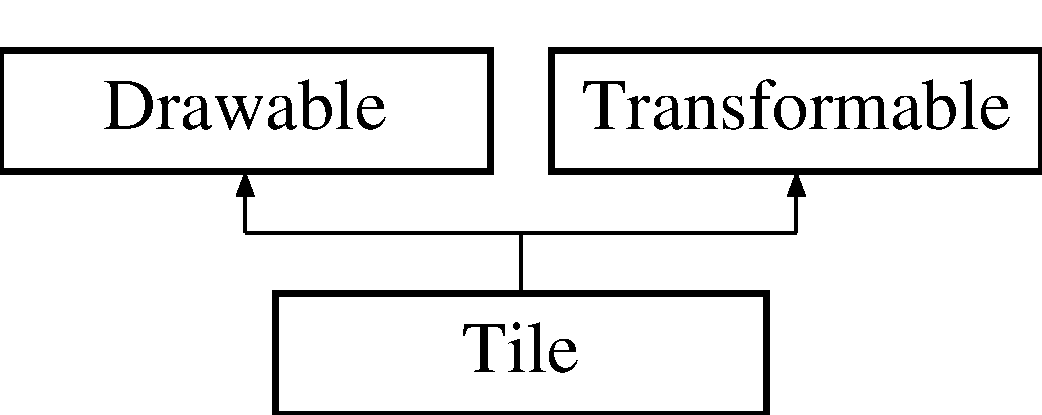
\includegraphics[height=2.000000cm]{df/d79/class_tile}
\end{center}
\end{figure}
\subsection*{Metody publiczne}
\begin{DoxyCompactItemize}
\item 
\mbox{\hyperlink{class_tile_aeeb5593bb6b75aae2edfcccbc84ab378}{Tile}} ()
\item 
void \mbox{\hyperlink{class_tile_a96ce55d5fcb4b12880531af2138ba6b2}{init}} ()
\item 
void \mbox{\hyperlink{class_tile_a8d009abca71750d7de775edea5910ab4}{infect}} (sf\+::\+Vector2f mouse\+Position)
\item 
void \mbox{\hyperlink{class_tile_a9f5897287ec33ef87fe88a2b254d1837}{remove}} ()
\item 
void \mbox{\hyperlink{class_tile_a89f236ddba83484658f4f68e117a786e}{add}} ()
\item 
\mbox{\hyperlink{class_tile_a98634abbd93fa13d0578d7103202d03d}{$\sim$\+Tile}} ()
\end{DoxyCompactItemize}
\subsection*{Metody prywatne}
\begin{DoxyCompactItemize}
\item 
void \mbox{\hyperlink{class_tile_a0d59a6e7e8b9c4236857470176edcf60}{update\+Positions}} ()
\item 
virtual void \mbox{\hyperlink{class_tile_acc7f60fb395569f318425129875336ca}{draw}} (sf\+::\+Render\+Target \&target, sf\+::\+Render\+States states) const
\end{DoxyCompactItemize}


\subsection{Opis szczegółowy}
Klasa służąca zarządzaniu całą siatką kwadratów. 

\subsection{Dokumentacja konstruktora i destruktora}
\mbox{\Hypertarget{class_tile_aeeb5593bb6b75aae2edfcccbc84ab378}\label{class_tile_aeeb5593bb6b75aae2edfcccbc84ab378}} 
\index{Tile@{Tile}!Tile@{Tile}}
\index{Tile@{Tile}!Tile@{Tile}}
\subsubsection{\texorpdfstring{Tile()}{Tile()}}
{\footnotesize\ttfamily Tile\+::\+Tile (\begin{DoxyParamCaption}{ }\end{DoxyParamCaption})}

Domyślny konstruktor 
\begin{DoxyCode}
6 \{
7 \}
\end{DoxyCode}
\mbox{\Hypertarget{class_tile_a98634abbd93fa13d0578d7103202d03d}\label{class_tile_a98634abbd93fa13d0578d7103202d03d}} 
\index{Tile@{Tile}!````~Tile@{$\sim$\+Tile}}
\index{````~Tile@{$\sim$\+Tile}!Tile@{Tile}}
\subsubsection{\texorpdfstring{$\sim$\+Tile()}{~Tile()}}
{\footnotesize\ttfamily Tile\+::$\sim$\+Tile (\begin{DoxyParamCaption}{ }\end{DoxyParamCaption})}

Destruktor 
\begin{DoxyCode}
120 \{
121 
122 \}
\end{DoxyCode}


\subsection{Dokumentacja funkcji składowych}
\mbox{\Hypertarget{class_tile_a89f236ddba83484658f4f68e117a786e}\label{class_tile_a89f236ddba83484658f4f68e117a786e}} 
\index{Tile@{Tile}!add@{add}}
\index{add@{add}!Tile@{Tile}}
\subsubsection{\texorpdfstring{add()}{add()}}
{\footnotesize\ttfamily void Tile\+::add (\begin{DoxyParamCaption}{ }\end{DoxyParamCaption})}

Metoda służąca dodawaniu komórek do siatki. Dodawana jest kolumna i wiersz na samych końcach. 
\begin{DoxyCode}
67 \{
68 
69     \textcolor{keywordflow}{if} (\mbox{\hyperlink{class_tile_settings_a003ae6e78b97855c8592b2b4c0818914}{TileSettings::getInstance}}()->tileSize.x == 
      \mbox{\hyperlink{class_tile_settings_a003ae6e78b97855c8592b2b4c0818914}{TileSettings::getInstance}}()->\mbox{\hyperlink{class_tile_settings_a2b24689813e0082b59df113b754778c2}{mainWindowSize}}.x || 
      \mbox{\hyperlink{class_tile_settings_a003ae6e78b97855c8592b2b4c0818914}{TileSettings::getInstance}}()->\mbox{\hyperlink{class_tile_settings_ae4be54be3619d21d536ce13b7354f165}{tileSize}}.y == 
      \mbox{\hyperlink{class_tile_settings_a003ae6e78b97855c8592b2b4c0818914}{TileSettings::getInstance}}()->\mbox{\hyperlink{class_tile_settings_a2b24689813e0082b59df113b754778c2}{mainWindowSize}}.y) \textcolor{keywordflow}{return};
70 
71     \textcolor{keywordflow}{if}(\mbox{\hyperlink{class_tile_settings_a003ae6e78b97855c8592b2b4c0818914}{TileSettings::getInstance}}()->tileQuads.empty())
72     \{
73         \mbox{\hyperlink{class_tile_settings_a003ae6e78b97855c8592b2b4c0818914}{TileSettings::getInstance}}()->\mbox{\hyperlink{class_tile_settings_ae4be54be3619d21d536ce13b7354f165}{tileSize}} = sf::Vector2u(1,1);
74         \mbox{\hyperlink{class_quad_settings_a20d7cfd0c56c11adcdf75c5e3011de67}{QuadSettings::getInstance}}()->\mbox{\hyperlink{class_quad_settings_abb4a967873d7a93098ef168b894280d6}{quadDimensions}} = sf::Vector2f(
      \mbox{\hyperlink{class_tile_settings_a003ae6e78b97855c8592b2b4c0818914}{TileSettings::getInstance}}()->mainWindowSize.x, 
      \mbox{\hyperlink{class_tile_settings_a003ae6e78b97855c8592b2b4c0818914}{TileSettings::getInstance}}()->\mbox{\hyperlink{class_tile_settings_a2b24689813e0082b59df113b754778c2}{mainWindowSize}}.y);
75         \mbox{\hyperlink{class_quad_settings_a20d7cfd0c56c11adcdf75c5e3011de67}{QuadSettings::getInstance}}()->\mbox{\hyperlink{class_quad_settings_a05e0e32535731778852480ab4c993cce}{updateTextures}}();
76         \mbox{\hyperlink{class_quad}{Quad}} quad;
77         quad.\mbox{\hyperlink{class_quad_a1f3970e8f264eabe131e20af7017f940}{setPosition}}(0, 0);
78         quad.\mbox{\hyperlink{class_quad_a35f20e65dd33bb5864f73575b04896e7}{getSprite}}()->setTextureRect(sf::IntRect(0, 0, 
      \mbox{\hyperlink{class_quad_settings_a20d7cfd0c56c11adcdf75c5e3011de67}{QuadSettings::getInstance}}()->quadDimensions.x, 
      \mbox{\hyperlink{class_quad_settings_a20d7cfd0c56c11adcdf75c5e3011de67}{QuadSettings::getInstance}}()->\mbox{\hyperlink{class_quad_settings_abb4a967873d7a93098ef168b894280d6}{quadDimensions}}.y));
79         \mbox{\hyperlink{class_tile_settings_a003ae6e78b97855c8592b2b4c0818914}{TileSettings::getInstance}}()->\mbox{\hyperlink{class_tile_settings_ac37d7b95a1e2266d38de0a70a907efb3}{tileQuads}}.push\_back(quad);
80 
81         \textcolor{keywordflow}{return};
82     \}
83 
84     \mbox{\hyperlink{class_tile_settings_a003ae6e78b97855c8592b2b4c0818914}{TileSettings::getInstance}}()->\mbox{\hyperlink{class_tile_settings_ae4be54be3619d21d536ce13b7354f165}{tileSize}} = sf::Vector2u(
      \mbox{\hyperlink{class_tile_settings_a003ae6e78b97855c8592b2b4c0818914}{TileSettings::getInstance}}()->tileSize.x, 
      \mbox{\hyperlink{class_tile_settings_a003ae6e78b97855c8592b2b4c0818914}{TileSettings::getInstance}}()->\mbox{\hyperlink{class_tile_settings_ae4be54be3619d21d536ce13b7354f165}{tileSize}}.y + 1);
85 
86     \textcolor{keywordflow}{for} (\textcolor{keywordtype}{unsigned} \textcolor{keywordtype}{int} i = 0; i < \mbox{\hyperlink{class_tile_settings_a003ae6e78b97855c8592b2b4c0818914}{TileSettings::getInstance}}()->
      \mbox{\hyperlink{class_tile_settings_ae4be54be3619d21d536ce13b7354f165}{tileSize}}.x; i++)
87     \{
88         \mbox{\hyperlink{class_quad}{Quad}} quad;
89         quad.\mbox{\hyperlink{class_quad_a1f3970e8f264eabe131e20af7017f940}{setPosition}}(i, \mbox{\hyperlink{class_tile_settings_a003ae6e78b97855c8592b2b4c0818914}{TileSettings::getInstance}}()->tileSize.y - 1
      );
90         \textcolor{keywordtype}{unsigned} \textcolor{keywordtype}{int} index = (\mbox{\hyperlink{class_tile_settings_a003ae6e78b97855c8592b2b4c0818914}{TileSettings::getInstance}}()->
      \mbox{\hyperlink{class_tile_settings_ae4be54be3619d21d536ce13b7354f165}{tileSize}}.y - 1) * (i + 1) + i;
91         \textcolor{keywordflow}{if}(index == \mbox{\hyperlink{class_tile_settings_a003ae6e78b97855c8592b2b4c0818914}{TileSettings::getInstance}}()->
      \mbox{\hyperlink{class_tile_settings_ac37d7b95a1e2266d38de0a70a907efb3}{tileQuads}}.size())
92         \{
93             \mbox{\hyperlink{class_tile_settings_a003ae6e78b97855c8592b2b4c0818914}{TileSettings::getInstance}}()->\mbox{\hyperlink{class_tile_settings_ac37d7b95a1e2266d38de0a70a907efb3}{tileQuads}}.push\_back(quad);
94         \}\textcolor{keywordflow}{else}
95         \{
96             \mbox{\hyperlink{class_tile_settings_a003ae6e78b97855c8592b2b4c0818914}{TileSettings::getInstance}}()->\mbox{\hyperlink{class_tile_settings_ac37d7b95a1e2266d38de0a70a907efb3}{tileQuads}}.insert(
      \mbox{\hyperlink{class_tile_settings_a003ae6e78b97855c8592b2b4c0818914}{TileSettings::getInstance}}()->tileQuads.begin() + index, quad);
97         \}
98     \}
99 
100     \mbox{\hyperlink{class_tile_settings_a003ae6e78b97855c8592b2b4c0818914}{TileSettings::getInstance}}()->\mbox{\hyperlink{class_tile_settings_ae4be54be3619d21d536ce13b7354f165}{tileSize}} = sf::Vector2u(
      \mbox{\hyperlink{class_tile_settings_a003ae6e78b97855c8592b2b4c0818914}{TileSettings::getInstance}}()->tileSize.x + 1, 
      \mbox{\hyperlink{class_tile_settings_a003ae6e78b97855c8592b2b4c0818914}{TileSettings::getInstance}}()->\mbox{\hyperlink{class_tile_settings_ae4be54be3619d21d536ce13b7354f165}{tileSize}}.y);
101 
102     \textcolor{keywordflow}{for} (\textcolor{keywordtype}{unsigned} \textcolor{keywordtype}{int} j = 0; j < \mbox{\hyperlink{class_tile_settings_a003ae6e78b97855c8592b2b4c0818914}{TileSettings::getInstance}}()->
      \mbox{\hyperlink{class_tile_settings_ae4be54be3619d21d536ce13b7354f165}{tileSize}}.y; j++)
103     \{
104         \mbox{\hyperlink{class_quad}{Quad}} quad;
105         quad.\mbox{\hyperlink{class_quad_a1f3970e8f264eabe131e20af7017f940}{setPosition}}(\mbox{\hyperlink{class_tile_settings_a003ae6e78b97855c8592b2b4c0818914}{TileSettings::getInstance}}()->tileSize.x - 1, j
      );
106         \mbox{\hyperlink{class_tile_settings_a003ae6e78b97855c8592b2b4c0818914}{TileSettings::getInstance}}()->\mbox{\hyperlink{class_tile_settings_ac37d7b95a1e2266d38de0a70a907efb3}{tileQuads}}.push\_back(quad);
107     \}
108 
109     \textcolor{comment}{// Dodanie tego do funkcji updatePosition();}
110     \mbox{\hyperlink{class_quad_settings_a20d7cfd0c56c11adcdf75c5e3011de67}{QuadSettings::getInstance}}()->\mbox{\hyperlink{class_quad_settings_abb4a967873d7a93098ef168b894280d6}{quadDimensions}} = sf::Vector2f(\textcolor{keywordtype}{float}
      (\mbox{\hyperlink{class_tile_settings_a003ae6e78b97855c8592b2b4c0818914}{TileSettings::getInstance}}()->mainWindowSize.x) / 
      \mbox{\hyperlink{class_tile_settings_a003ae6e78b97855c8592b2b4c0818914}{TileSettings::getInstance}}()->\mbox{\hyperlink{class_tile_settings_ae4be54be3619d21d536ce13b7354f165}{tileSize}}.x, \textcolor{keywordtype}{float}(
      \mbox{\hyperlink{class_tile_settings_a003ae6e78b97855c8592b2b4c0818914}{TileSettings::getInstance}}()->\mbox{\hyperlink{class_tile_settings_a2b24689813e0082b59df113b754778c2}{mainWindowSize}}.y) / 
      \mbox{\hyperlink{class_tile_settings_a003ae6e78b97855c8592b2b4c0818914}{TileSettings::getInstance}}()->\mbox{\hyperlink{class_tile_settings_ae4be54be3619d21d536ce13b7354f165}{tileSize}}.y);
111     \mbox{\hyperlink{class_quad_settings_a20d7cfd0c56c11adcdf75c5e3011de67}{QuadSettings::getInstance}}()->\mbox{\hyperlink{class_quad_settings_a05e0e32535731778852480ab4c993cce}{updateTextures}}();
112 
113     \mbox{\hyperlink{class_tile_a0d59a6e7e8b9c4236857470176edcf60}{updatePositions}}();
114 
115 
116 \}
\end{DoxyCode}
\mbox{\Hypertarget{class_tile_acc7f60fb395569f318425129875336ca}\label{class_tile_acc7f60fb395569f318425129875336ca}} 
\index{Tile@{Tile}!draw@{draw}}
\index{draw@{draw}!Tile@{Tile}}
\subsubsection{\texorpdfstring{draw()}{draw()}}
{\footnotesize\ttfamily virtual void Tile\+::draw (\begin{DoxyParamCaption}\item[{sf\+::\+Render\+Target \&}]{target,  }\item[{sf\+::\+Render\+States}]{states }\end{DoxyParamCaption}) const\hspace{0.3cm}{\ttfamily [inline]}, {\ttfamily [private]}, {\ttfamily [virtual]}}

Metoda, która została nadpisana z sf\+::\+Drawable


\begin{DoxyParams}{Parametry}
{\em target} & Render\+Target do którego będzie rysowane \\
\hline
{\em states} & Aktualny stan rysowania \\
\hline
\end{DoxyParams}

\begin{DoxyCode}
54     \{
55         states.transform *= getTransform();
56 
57         \textcolor{keywordflow}{for} (\textcolor{keyword}{auto} &element : \mbox{\hyperlink{class_tile_settings_a003ae6e78b97855c8592b2b4c0818914}{TileSettings::getInstance}}()->tileQuads) \{
58             \textcolor{keywordflow}{if}(!\mbox{\hyperlink{class_simulation_settings_ab69bcd8bb611656b17d1f655d09a3004}{SimulationSettings::getInstance}}()->stopLogic && !element.
      healthy)
59             \{
60                 element.updateState();
61             \}
62             target.draw(*element.getSprite(), states);
63         \}
64 
65     \}
\end{DoxyCode}
\mbox{\Hypertarget{class_tile_a8d009abca71750d7de775edea5910ab4}\label{class_tile_a8d009abca71750d7de775edea5910ab4}} 
\index{Tile@{Tile}!infect@{infect}}
\index{infect@{infect}!Tile@{Tile}}
\subsubsection{\texorpdfstring{infect()}{infect()}}
{\footnotesize\ttfamily void Tile\+::infect (\begin{DoxyParamCaption}\item[{sf\+::\+Vector2f}]{mouse\+Position }\end{DoxyParamCaption})}

Metoda służąca infekowaniu komórki


\begin{DoxyParams}{Parametry}
{\em mouse\+Position} & Aktualna pozycja kursora na planszy. \\
\hline
\end{DoxyParams}

\begin{DoxyCode}
34 \{
35     \textcolor{keywordflow}{for} (\textcolor{keyword}{auto} &element : \mbox{\hyperlink{class_tile_settings_a003ae6e78b97855c8592b2b4c0818914}{TileSettings::getInstance}}()->tileQuads) \{
36         \textcolor{keywordflow}{if} (element.getSprite()->getGlobalBounds().contains(mousePosition) \textcolor{comment}{/*&& element.healthy */}) \{
37             \textcolor{keywordflow}{if}(\mbox{\hyperlink{class_simulation_settings_ab69bcd8bb611656b17d1f655d09a3004}{SimulationSettings::getInstance}}()->
      \mbox{\hyperlink{class_simulation_settings_a3cf918e098904961a658c38047f607fd}{pointOfInfection}})element.pointOfInfection = \textcolor{keyword}{true};
38             element.setInfected();
39         \}
40     \}
41 \}
\end{DoxyCode}
\mbox{\Hypertarget{class_tile_a96ce55d5fcb4b12880531af2138ba6b2}\label{class_tile_a96ce55d5fcb4b12880531af2138ba6b2}} 
\index{Tile@{Tile}!init@{init}}
\index{init@{init}!Tile@{Tile}}
\subsubsection{\texorpdfstring{init()}{init()}}
{\footnotesize\ttfamily void Tile\+::init (\begin{DoxyParamCaption}{ }\end{DoxyParamCaption})}

Metoda służąca inicjacji zmiennych oraz domyślnej siatki. 
\begin{DoxyCode}
10 \{
11 
12     \mbox{\hyperlink{class_tile_settings_a003ae6e78b97855c8592b2b4c0818914}{TileSettings::getInstance}}()->\mbox{\hyperlink{class_tile_settings_ae4be54be3619d21d536ce13b7354f165}{tileSize}} = sf::Vector2u(
      \mbox{\hyperlink{class_tile_settings_a003ae6e78b97855c8592b2b4c0818914}{TileSettings::getInstance}}()->mainWindowSize.x/
      \mbox{\hyperlink{class_quad_settings_a20d7cfd0c56c11adcdf75c5e3011de67}{QuadSettings::getInstance}}()->\mbox{\hyperlink{class_quad_settings_abb4a967873d7a93098ef168b894280d6}{quadDimensions}}.x,
13         \mbox{\hyperlink{class_tile_settings_a003ae6e78b97855c8592b2b4c0818914}{TileSettings::getInstance}}()->\mbox{\hyperlink{class_tile_settings_a2b24689813e0082b59df113b754778c2}{mainWindowSize}}.y / 
      \mbox{\hyperlink{class_quad_settings_a20d7cfd0c56c11adcdf75c5e3011de67}{QuadSettings::getInstance}}()->\mbox{\hyperlink{class_quad_settings_abb4a967873d7a93098ef168b894280d6}{quadDimensions}}.y);
14     \mbox{\hyperlink{class_tile_settings_a003ae6e78b97855c8592b2b4c0818914}{TileSettings::getInstance}}()->\mbox{\hyperlink{class_tile_settings_ac37d7b95a1e2266d38de0a70a907efb3}{tileQuads}}.clear();
15     \mbox{\hyperlink{class_tile_settings_a003ae6e78b97855c8592b2b4c0818914}{TileSettings::getInstance}}()->\mbox{\hyperlink{class_tile_settings_ac37d7b95a1e2266d38de0a70a907efb3}{tileQuads}}.shrink\_to\_fit();
16     \mbox{\hyperlink{class_tile_settings_a003ae6e78b97855c8592b2b4c0818914}{TileSettings::getInstance}}()->\mbox{\hyperlink{class_tile_settings_ac37d7b95a1e2266d38de0a70a907efb3}{tileQuads}}.reserve(
      \mbox{\hyperlink{class_tile_settings_a003ae6e78b97855c8592b2b4c0818914}{TileSettings::getInstance}}()->tileSize.x * 
      \mbox{\hyperlink{class_tile_settings_a003ae6e78b97855c8592b2b4c0818914}{TileSettings::getInstance}}()->\mbox{\hyperlink{class_tile_settings_ae4be54be3619d21d536ce13b7354f165}{tileSize}}.y);
17 
18     \mbox{\hyperlink{class_quad_settings_a20d7cfd0c56c11adcdf75c5e3011de67}{QuadSettings::getInstance}}()->\mbox{\hyperlink{class_quad_settings_a05e0e32535731778852480ab4c993cce}{updateTextures}}();
19 
20        \textcolor{keywordflow}{for}(\textcolor{keywordtype}{unsigned} \textcolor{keywordtype}{int} i = 0; i < \mbox{\hyperlink{class_tile_settings_a003ae6e78b97855c8592b2b4c0818914}{TileSettings::getInstance}}()->
      \mbox{\hyperlink{class_tile_settings_ae4be54be3619d21d536ce13b7354f165}{tileSize}}.x; i++)
21        \{
22            \textcolor{keywordflow}{for}(\textcolor{keywordtype}{unsigned} \textcolor{keywordtype}{int} j = 0; j < \mbox{\hyperlink{class_tile_settings_a003ae6e78b97855c8592b2b4c0818914}{TileSettings::getInstance}}()->
      \mbox{\hyperlink{class_tile_settings_ae4be54be3619d21d536ce13b7354f165}{tileSize}}.y; j++)
23            \{
24                \mbox{\hyperlink{class_quad}{Quad}} quad;
25                quad.\mbox{\hyperlink{class_quad_a1f3970e8f264eabe131e20af7017f940}{setPosition}}(i, j);
26                \mbox{\hyperlink{class_tile_settings_a003ae6e78b97855c8592b2b4c0818914}{TileSettings::getInstance}}()->\mbox{\hyperlink{class_tile_settings_ac37d7b95a1e2266d38de0a70a907efb3}{tileQuads}}.push\_back(quad);
27            \}
28        \}
29 
30     
31 \}
\end{DoxyCode}
\mbox{\Hypertarget{class_tile_a9f5897287ec33ef87fe88a2b254d1837}\label{class_tile_a9f5897287ec33ef87fe88a2b254d1837}} 
\index{Tile@{Tile}!remove@{remove}}
\index{remove@{remove}!Tile@{Tile}}
\subsubsection{\texorpdfstring{remove()}{remove()}}
{\footnotesize\ttfamily void Tile\+::remove (\begin{DoxyParamCaption}{ }\end{DoxyParamCaption})}

Metoda służąca usuwaniu komórek z siatki. Usuwana jest ostatnia kolumna i wiersz. 
\begin{DoxyCode}
44 \{
45 
46     \textcolor{keywordflow}{if} (\mbox{\hyperlink{class_tile_settings_a003ae6e78b97855c8592b2b4c0818914}{TileSettings::getInstance}}()->tileSize.x == 0 || 
      \mbox{\hyperlink{class_tile_settings_a003ae6e78b97855c8592b2b4c0818914}{TileSettings::getInstance}}()->\mbox{\hyperlink{class_tile_settings_ae4be54be3619d21d536ce13b7354f165}{tileSize}}.y == 0) \textcolor{keywordflow}{return};
47 
48 
49     \mbox{\hyperlink{class_tile_settings_a003ae6e78b97855c8592b2b4c0818914}{TileSettings::getInstance}}()->\mbox{\hyperlink{class_tile_settings_ac37d7b95a1e2266d38de0a70a907efb3}{tileQuads}}.erase(
      \mbox{\hyperlink{class_tile_settings_a003ae6e78b97855c8592b2b4c0818914}{TileSettings::getInstance}}()->tileQuads.end() - 
      \mbox{\hyperlink{class_tile_settings_a003ae6e78b97855c8592b2b4c0818914}{TileSettings::getInstance}}()->\mbox{\hyperlink{class_tile_settings_ae4be54be3619d21d536ce13b7354f165}{tileSize}}.y, 
      \mbox{\hyperlink{class_tile_settings_a003ae6e78b97855c8592b2b4c0818914}{TileSettings::getInstance}}()->\mbox{\hyperlink{class_tile_settings_ac37d7b95a1e2266d38de0a70a907efb3}{tileQuads}}.end());
50     \mbox{\hyperlink{class_tile_settings_a003ae6e78b97855c8592b2b4c0818914}{TileSettings::getInstance}}()->\mbox{\hyperlink{class_tile_settings_ac37d7b95a1e2266d38de0a70a907efb3}{tileQuads}}.shrink\_to\_fit();
51     \textcolor{keywordflow}{for} (\textcolor{keywordtype}{unsigned} \textcolor{keywordtype}{int} i = 0; i < \mbox{\hyperlink{class_tile_settings_a003ae6e78b97855c8592b2b4c0818914}{TileSettings::getInstance}}()->
      \mbox{\hyperlink{class_tile_settings_ae4be54be3619d21d536ce13b7354f165}{tileSize}}.y - 1; i++)
52     \{
53         \textcolor{keywordtype}{int} index = \mbox{\hyperlink{class_tile_settings_a003ae6e78b97855c8592b2b4c0818914}{TileSettings::getInstance}}()->
      \mbox{\hyperlink{class_tile_settings_ae4be54be3619d21d536ce13b7354f165}{tileSize}}.y + i * \mbox{\hyperlink{class_tile_settings_a003ae6e78b97855c8592b2b4c0818914}{TileSettings::getInstance}}()->
      \mbox{\hyperlink{class_tile_settings_ae4be54be3619d21d536ce13b7354f165}{tileSize}}.y - (i + 1);
54         \mbox{\hyperlink{class_tile_settings_a003ae6e78b97855c8592b2b4c0818914}{TileSettings::getInstance}}()->\mbox{\hyperlink{class_tile_settings_ac37d7b95a1e2266d38de0a70a907efb3}{tileQuads}}.erase(
      \mbox{\hyperlink{class_tile_settings_a003ae6e78b97855c8592b2b4c0818914}{TileSettings::getInstance}}()->tileQuads.begin() + index);
55     \}
56     \mbox{\hyperlink{class_tile_settings_a003ae6e78b97855c8592b2b4c0818914}{TileSettings::getInstance}}()->\mbox{\hyperlink{class_tile_settings_ac37d7b95a1e2266d38de0a70a907efb3}{tileQuads}}.shrink\_to\_fit();
57     \mbox{\hyperlink{class_tile_settings_a003ae6e78b97855c8592b2b4c0818914}{TileSettings::getInstance}}()->\mbox{\hyperlink{class_tile_settings_ae4be54be3619d21d536ce13b7354f165}{tileSize}} = sf::Vector2u(
      \mbox{\hyperlink{class_tile_settings_a003ae6e78b97855c8592b2b4c0818914}{TileSettings::getInstance}}()->tileSize.x -1, 
      \mbox{\hyperlink{class_tile_settings_a003ae6e78b97855c8592b2b4c0818914}{TileSettings::getInstance}}()->\mbox{\hyperlink{class_tile_settings_ae4be54be3619d21d536ce13b7354f165}{tileSize}}.y -1);
58 
59     \mbox{\hyperlink{class_quad_settings_a20d7cfd0c56c11adcdf75c5e3011de67}{QuadSettings::getInstance}}()->\mbox{\hyperlink{class_quad_settings_abb4a967873d7a93098ef168b894280d6}{quadDimensions}} = sf::Vector2f(\textcolor{keywordtype}{float}
      (\mbox{\hyperlink{class_tile_settings_a003ae6e78b97855c8592b2b4c0818914}{TileSettings::getInstance}}()->mainWindowSize.x) / 
      \mbox{\hyperlink{class_tile_settings_a003ae6e78b97855c8592b2b4c0818914}{TileSettings::getInstance}}()->\mbox{\hyperlink{class_tile_settings_ae4be54be3619d21d536ce13b7354f165}{tileSize}}.x, \textcolor{keywordtype}{float}(
      \mbox{\hyperlink{class_tile_settings_a003ae6e78b97855c8592b2b4c0818914}{TileSettings::getInstance}}()->\mbox{\hyperlink{class_tile_settings_a2b24689813e0082b59df113b754778c2}{mainWindowSize}}.y) / 
      \mbox{\hyperlink{class_tile_settings_a003ae6e78b97855c8592b2b4c0818914}{TileSettings::getInstance}}()->\mbox{\hyperlink{class_tile_settings_ae4be54be3619d21d536ce13b7354f165}{tileSize}}.y);
60     \mbox{\hyperlink{class_quad_settings_a20d7cfd0c56c11adcdf75c5e3011de67}{QuadSettings::getInstance}}()->\mbox{\hyperlink{class_quad_settings_a05e0e32535731778852480ab4c993cce}{updateTextures}}();
61 
62     \mbox{\hyperlink{class_tile_a0d59a6e7e8b9c4236857470176edcf60}{updatePositions}}();
63     
64 \}
\end{DoxyCode}
\mbox{\Hypertarget{class_tile_a0d59a6e7e8b9c4236857470176edcf60}\label{class_tile_a0d59a6e7e8b9c4236857470176edcf60}} 
\index{Tile@{Tile}!update\+Positions@{update\+Positions}}
\index{update\+Positions@{update\+Positions}!Tile@{Tile}}
\subsubsection{\texorpdfstring{update\+Positions()}{updatePositions()}}
{\footnotesize\ttfamily void Tile\+::update\+Positions (\begin{DoxyParamCaption}{ }\end{DoxyParamCaption})\hspace{0.3cm}{\ttfamily [private]}}

Metoda służąca aktualizacji pozycji komórek na planszy oraz ich rozmiaru. 
\begin{DoxyCode}
125 \{
126     \textcolor{keywordflow}{for} (\textcolor{keywordtype}{unsigned} \textcolor{keywordtype}{int} i = 0; i < \mbox{\hyperlink{class_tile_settings_a003ae6e78b97855c8592b2b4c0818914}{TileSettings::getInstance}}()->
      \mbox{\hyperlink{class_tile_settings_ae4be54be3619d21d536ce13b7354f165}{tileSize}}.x; i++)
127     \{
128         \textcolor{keywordflow}{for} (\textcolor{keywordtype}{unsigned} \textcolor{keywordtype}{int} j = 0; j < \mbox{\hyperlink{class_tile_settings_a003ae6e78b97855c8592b2b4c0818914}{TileSettings::getInstance}}()->
      \mbox{\hyperlink{class_tile_settings_ae4be54be3619d21d536ce13b7354f165}{tileSize}}.y; j++)
129         \{
130             \mbox{\hyperlink{class_quad}{Quad}} *quad = &\mbox{\hyperlink{class_tile_settings_a003ae6e78b97855c8592b2b4c0818914}{TileSettings::getInstance}}()->
      \mbox{\hyperlink{class_tile_settings_ac37d7b95a1e2266d38de0a70a907efb3}{tileQuads}}.at(j + i * \mbox{\hyperlink{class_tile_settings_a003ae6e78b97855c8592b2b4c0818914}{TileSettings::getInstance}}()->tileSize.y);
131             quad->\mbox{\hyperlink{class_quad_a1f3970e8f264eabe131e20af7017f940}{setPosition}}(i, j);
132             quad->\mbox{\hyperlink{class_quad_a35f20e65dd33bb5864f73575b04896e7}{getSprite}}()->setTextureRect(sf::IntRect(0, 0, 
      \mbox{\hyperlink{class_quad_settings_a20d7cfd0c56c11adcdf75c5e3011de67}{QuadSettings::getInstance}}()->quadDimensions.x, 
      \mbox{\hyperlink{class_quad_settings_a20d7cfd0c56c11adcdf75c5e3011de67}{QuadSettings::getInstance}}()->\mbox{\hyperlink{class_quad_settings_abb4a967873d7a93098ef168b894280d6}{quadDimensions}}.y));
133             \textcolor{keywordflow}{if} (quad->\mbox{\hyperlink{class_quad_ae439ca631a9f51147b9d84a9c9df49c4}{infected}}) quad->\mbox{\hyperlink{class_quad_a67483d3d113d177c0820f586a923e65e}{updateNearbyElements}}();
134         \}
135     \}
136 \}
\end{DoxyCode}


Dokumentacja dla tej klasy została wygenerowana z plików\+:\begin{DoxyCompactItemize}
\item 
\mbox{\hyperlink{_tile_8h}{Tile.\+h}}\item 
\mbox{\hyperlink{_tile_8cpp}{Tile.\+cpp}}\end{DoxyCompactItemize}

\hypertarget{class_tile_settings}{}\section{Dokumentacja klasy Tile\+Settings}
\label{class_tile_settings}\index{Tile\+Settings@{Tile\+Settings}}


{\ttfamily \#include $<$Tile\+Settings.\+h$>$}

\subsection*{Statyczne metody publiczne}
\begin{DoxyCompactItemize}
\item 
static \mbox{\hyperlink{class_tile_settings}{Tile\+Settings}} $\ast$ \mbox{\hyperlink{class_tile_settings_a003ae6e78b97855c8592b2b4c0818914}{get\+Instance}} ()
\end{DoxyCompactItemize}
\subsection*{Atrybuty publiczne}
\begin{DoxyCompactItemize}
\item 
sf\+::\+Vector2u \mbox{\hyperlink{class_tile_settings_ae4be54be3619d21d536ce13b7354f165}{tile\+Size}}
\item 
std\+::vector$<$ \mbox{\hyperlink{class_quad}{Quad}} $>$ \mbox{\hyperlink{class_tile_settings_ac37d7b95a1e2266d38de0a70a907efb3}{tile\+Quads}}
\item 
sf\+::\+Vector2u \mbox{\hyperlink{class_tile_settings_a2b24689813e0082b59df113b754778c2}{main\+Window\+Size}}
\end{DoxyCompactItemize}
\subsection*{Metody prywatne}
\begin{DoxyCompactItemize}
\item 
\mbox{\hyperlink{class_tile_settings_a5903073619b7b4bf85a2dc3548db84fe}{Tile\+Settings}} ()
\item 
\mbox{\hyperlink{class_tile_settings_a4e8a5a736c71cec9e60a49d5cafca150}{$\sim$\+Tile\+Settings}} ()
\end{DoxyCompactItemize}
\subsection*{Statyczne atrybuty prywatne}
\begin{DoxyCompactItemize}
\item 
static \mbox{\hyperlink{class_tile_settings}{Tile\+Settings}} $\ast$ \mbox{\hyperlink{class_tile_settings_a4e06ef1c8909d1e22f82976b9b4162f0}{s\+\_\+tile\+\_\+settings}} = nullptr
\end{DoxyCompactItemize}


\subsection{Opis szczegółowy}
Singleton odpowiadający za ustawienia siatki komórek. Przechowuje najważniejsze zmienne. 

\subsection{Dokumentacja konstruktora i destruktora}
\mbox{\Hypertarget{class_tile_settings_a5903073619b7b4bf85a2dc3548db84fe}\label{class_tile_settings_a5903073619b7b4bf85a2dc3548db84fe}} 
\index{Tile\+Settings@{Tile\+Settings}!Tile\+Settings@{Tile\+Settings}}
\index{Tile\+Settings@{Tile\+Settings}!Tile\+Settings@{Tile\+Settings}}
\subsubsection{\texorpdfstring{Tile\+Settings()}{TileSettings()}}
{\footnotesize\ttfamily Tile\+Settings\+::\+Tile\+Settings (\begin{DoxyParamCaption}{ }\end{DoxyParamCaption})\hspace{0.3cm}{\ttfamily [private]}}

Domyślny konstruktor. 
\begin{DoxyCode}
13 \{
14     \mbox{\hyperlink{class_tile_settings_ac37d7b95a1e2266d38de0a70a907efb3}{tileQuads}}.clear();
15     \mbox{\hyperlink{class_tile_settings_ac37d7b95a1e2266d38de0a70a907efb3}{tileQuads}}.shrink\_to\_fit();
16 
17     \mbox{\hyperlink{class_tile_settings_ae4be54be3619d21d536ce13b7354f165}{tileSize}} = sf::Vector2u(0, 0);
18 
19     \mbox{\hyperlink{class_tile_settings_a2b24689813e0082b59df113b754778c2}{mainWindowSize}} = sf::Vector2u(0, 0);
20 \}
\end{DoxyCode}
\mbox{\Hypertarget{class_tile_settings_a4e8a5a736c71cec9e60a49d5cafca150}\label{class_tile_settings_a4e8a5a736c71cec9e60a49d5cafca150}} 
\index{Tile\+Settings@{Tile\+Settings}!````~Tile\+Settings@{$\sim$\+Tile\+Settings}}
\index{````~Tile\+Settings@{$\sim$\+Tile\+Settings}!Tile\+Settings@{Tile\+Settings}}
\subsubsection{\texorpdfstring{$\sim$\+Tile\+Settings()}{~TileSettings()}}
{\footnotesize\ttfamily Tile\+Settings\+::$\sim$\+Tile\+Settings (\begin{DoxyParamCaption}{ }\end{DoxyParamCaption})\hspace{0.3cm}{\ttfamily [private]}}

Destruktor. 
\begin{DoxyCode}
24 \{
25     \textcolor{keyword}{delete} \mbox{\hyperlink{class_tile_settings_a4e06ef1c8909d1e22f82976b9b4162f0}{s\_tile\_settings}};
26 \}
\end{DoxyCode}


\subsection{Dokumentacja funkcji składowych}
\mbox{\Hypertarget{class_tile_settings_a003ae6e78b97855c8592b2b4c0818914}\label{class_tile_settings_a003ae6e78b97855c8592b2b4c0818914}} 
\index{Tile\+Settings@{Tile\+Settings}!get\+Instance@{get\+Instance}}
\index{get\+Instance@{get\+Instance}!Tile\+Settings@{Tile\+Settings}}
\subsubsection{\texorpdfstring{get\+Instance()}{getInstance()}}
{\footnotesize\ttfamily \mbox{\hyperlink{class_tile_settings}{Tile\+Settings}} $\ast$ Tile\+Settings\+::get\+Instance (\begin{DoxyParamCaption}{ }\end{DoxyParamCaption})\hspace{0.3cm}{\ttfamily [static]}}

Metoda zwracająca instancje klasy. \begin{DoxyReturn}{Zwraca}
Tile\+Settings$\ast$ 
\end{DoxyReturn}

\begin{DoxyCode}
6 \{
7     \textcolor{keywordflow}{if} (!\mbox{\hyperlink{class_tile_settings_a4e06ef1c8909d1e22f82976b9b4162f0}{s\_tile\_settings}})
8         \mbox{\hyperlink{class_tile_settings_a4e06ef1c8909d1e22f82976b9b4162f0}{s\_tile\_settings}} = \textcolor{keyword}{new} \mbox{\hyperlink{class_tile_settings_a5903073619b7b4bf85a2dc3548db84fe}{TileSettings}}();
9     \textcolor{keywordflow}{return} \mbox{\hyperlink{class_tile_settings_a4e06ef1c8909d1e22f82976b9b4162f0}{s\_tile\_settings}};
10 \}
\end{DoxyCode}


\subsection{Dokumentacja atrybutów składowych}
\mbox{\Hypertarget{class_tile_settings_a2b24689813e0082b59df113b754778c2}\label{class_tile_settings_a2b24689813e0082b59df113b754778c2}} 
\index{Tile\+Settings@{Tile\+Settings}!main\+Window\+Size@{main\+Window\+Size}}
\index{main\+Window\+Size@{main\+Window\+Size}!Tile\+Settings@{Tile\+Settings}}
\subsubsection{\texorpdfstring{main\+Window\+Size}{mainWindowSize}}
{\footnotesize\ttfamily sf\+::\+Vector2u Tile\+Settings\+::main\+Window\+Size}

Zmienna przechowująca rozmiar głównego okna. \mbox{\Hypertarget{class_tile_settings_a4e06ef1c8909d1e22f82976b9b4162f0}\label{class_tile_settings_a4e06ef1c8909d1e22f82976b9b4162f0}} 
\index{Tile\+Settings@{Tile\+Settings}!s\+\_\+tile\+\_\+settings@{s\+\_\+tile\+\_\+settings}}
\index{s\+\_\+tile\+\_\+settings@{s\+\_\+tile\+\_\+settings}!Tile\+Settings@{Tile\+Settings}}
\subsubsection{\texorpdfstring{s\+\_\+tile\+\_\+settings}{s\_tile\_settings}}
{\footnotesize\ttfamily \mbox{\hyperlink{class_tile_settings}{Tile\+Settings}} $\ast$ Tile\+Settings\+::s\+\_\+tile\+\_\+settings = nullptr\hspace{0.3cm}{\ttfamily [static]}, {\ttfamily [private]}}

Jedyna instancja klasy \mbox{\hyperlink{class_tile_settings}{Tile\+Settings}}, która jest udostępniana przez static Tile\+Settings$\ast$ \mbox{\hyperlink{class_tile_settings_a003ae6e78b97855c8592b2b4c0818914}{Tile\+Settings\+::get\+Instance()}} \mbox{\Hypertarget{class_tile_settings_ac37d7b95a1e2266d38de0a70a907efb3}\label{class_tile_settings_ac37d7b95a1e2266d38de0a70a907efb3}} 
\index{Tile\+Settings@{Tile\+Settings}!tile\+Quads@{tile\+Quads}}
\index{tile\+Quads@{tile\+Quads}!Tile\+Settings@{Tile\+Settings}}
\subsubsection{\texorpdfstring{tile\+Quads}{tileQuads}}
{\footnotesize\ttfamily std\+::vector$<$\mbox{\hyperlink{class_quad}{Quad}}$>$ Tile\+Settings\+::tile\+Quads}

Wektor przechowujący wszystkie komórki. \mbox{\Hypertarget{class_tile_settings_ae4be54be3619d21d536ce13b7354f165}\label{class_tile_settings_ae4be54be3619d21d536ce13b7354f165}} 
\index{Tile\+Settings@{Tile\+Settings}!tile\+Size@{tile\+Size}}
\index{tile\+Size@{tile\+Size}!Tile\+Settings@{Tile\+Settings}}
\subsubsection{\texorpdfstring{tile\+Size}{tileSize}}
{\footnotesize\ttfamily sf\+::\+Vector2u Tile\+Settings\+::tile\+Size}

Zmienna opisująca szerokość i długość siatki. 

Dokumentacja dla tej klasy została wygenerowana z plików\+:\begin{DoxyCompactItemize}
\item 
\mbox{\hyperlink{_tile_settings_8h}{Tile\+Settings.\+h}}\item 
\mbox{\hyperlink{_tile_settings_8cpp}{Tile\+Settings.\+cpp}}\end{DoxyCompactItemize}

\hypertarget{class_utility}{}\section{Dokumentacja klasy Utility}
\label{class_utility}\index{Utility@{Utility}}


{\ttfamily \#include $<$Utility.\+h$>$}

\subsection*{Metody publiczne}
\begin{DoxyCompactItemize}
\item 
\mbox{\hyperlink{class_utility_ac7af3e1642ac8d53ef180180a08fbd00}{Utility}} ()
\item 
\mbox{\hyperlink{class_utility_aecfe4b31e39b00555158a2d8288b874a}{$\sim$\+Utility}} ()
\item 
bool \mbox{\hyperlink{class_utility_a1737e13071619724884c55559c34d727}{yes\+Or\+No}} (float probability)
\item 
void \mbox{\hyperlink{class_utility_ae89bf9504ce0848783234853483da262}{generate\+Nearby\+Elements}} (std\+::vector$<$ \mbox{\hyperlink{class_quad}{Quad}} $>$ $\ast$tile\+Quads, std\+::vector$<$ \mbox{\hyperlink{class_quad}{Quad}} $\ast$$>$ $\ast$nearby\+Quads, sf\+::\+Vector2u tile\+Size, sf\+::\+Vector2u position)
\item 
bool \mbox{\hyperlink{class_utility_a535e980c2716b8118deb78bef51079da}{clicked\+In\+Window}} (sf\+::\+Vector2f window\+Size, sf\+::\+Vector2f window\+Position, sf\+::\+Vector2u mouse\+Position)
\item 
void \mbox{\hyperlink{class_utility_a8aafe3b77344b4d230c431cbd64b09dc}{all\+Divisors}} (std\+::vector$<$ std\+::string $>$ $\ast$v\+\_\+factors)
\end{DoxyCompactItemize}
\subsection*{Metody prywatne}
\begin{DoxyCompactItemize}
\item 
bool \mbox{\hyperlink{class_utility_a65721c1ad255c50823139ad357212a13}{exist\+Quad}} (sf\+::\+Vector2u point, sf\+::\+Vector2u tile\+Size)
\end{DoxyCompactItemize}


\subsection{Opis szczegółowy}
Klasa posiadająca podręczne metody dla symulacji. 

\subsection{Dokumentacja konstruktora i destruktora}
\mbox{\Hypertarget{class_utility_ac7af3e1642ac8d53ef180180a08fbd00}\label{class_utility_ac7af3e1642ac8d53ef180180a08fbd00}} 
\index{Utility@{Utility}!Utility@{Utility}}
\index{Utility@{Utility}!Utility@{Utility}}
\subsubsection{\texorpdfstring{Utility()}{Utility()}}
{\footnotesize\ttfamily Utility\+::\+Utility (\begin{DoxyParamCaption}{ }\end{DoxyParamCaption})}

Domyślny konstruktor. 
\begin{DoxyCode}
7 \{
8 \}
\end{DoxyCode}
\mbox{\Hypertarget{class_utility_aecfe4b31e39b00555158a2d8288b874a}\label{class_utility_aecfe4b31e39b00555158a2d8288b874a}} 
\index{Utility@{Utility}!````~Utility@{$\sim$\+Utility}}
\index{````~Utility@{$\sim$\+Utility}!Utility@{Utility}}
\subsubsection{\texorpdfstring{$\sim$\+Utility()}{~Utility()}}
{\footnotesize\ttfamily Utility\+::$\sim$\+Utility (\begin{DoxyParamCaption}{ }\end{DoxyParamCaption})}

Destruktor. 
\begin{DoxyCode}
12 \{
13 \}
\end{DoxyCode}


\subsection{Dokumentacja funkcji składowych}
\mbox{\Hypertarget{class_utility_a8aafe3b77344b4d230c431cbd64b09dc}\label{class_utility_a8aafe3b77344b4d230c431cbd64b09dc}} 
\index{Utility@{Utility}!all\+Divisors@{all\+Divisors}}
\index{all\+Divisors@{all\+Divisors}!Utility@{Utility}}
\subsubsection{\texorpdfstring{all\+Divisors()}{allDivisors()}}
{\footnotesize\ttfamily void Utility\+::all\+Divisors (\begin{DoxyParamCaption}\item[{std\+::vector$<$ std\+::string $>$ $\ast$}]{v\+\_\+factors }\end{DoxyParamCaption})}

Metoda oblicza wszystkie wspólne dzielniki szerokości i długośći głównego okna. 
\begin{DoxyParams}{Parametry}
{\em $\ast$v\+\_\+factors} & wskaźnik do wektora stringów \\
\hline
\end{DoxyParams}

\begin{DoxyCode}
59 \{
60     \textcolor{keywordtype}{int} n, m;
61 
62 
63     v\_factors->clear();
64     v\_factors->shrink\_to\_fit();
65 
66 
67     \textcolor{keywordflow}{if}(\mbox{\hyperlink{class_tile_settings_a003ae6e78b97855c8592b2b4c0818914}{TileSettings::getInstance}}()->mainWindowSize.x > 
      \mbox{\hyperlink{class_tile_settings_a003ae6e78b97855c8592b2b4c0818914}{TileSettings::getInstance}}()->\mbox{\hyperlink{class_tile_settings_a2b24689813e0082b59df113b754778c2}{mainWindowSize}}.y )
68     \{
69         m = \mbox{\hyperlink{class_tile_settings_a003ae6e78b97855c8592b2b4c0818914}{TileSettings::getInstance}}()->\mbox{\hyperlink{class_tile_settings_a2b24689813e0082b59df113b754778c2}{mainWindowSize}}.x;
70         n = \mbox{\hyperlink{class_tile_settings_a003ae6e78b97855c8592b2b4c0818914}{TileSettings::getInstance}}()->\mbox{\hyperlink{class_tile_settings_a2b24689813e0082b59df113b754778c2}{mainWindowSize}}.y;
71     \}\textcolor{keywordflow}{else}
72     \{
73         n = \mbox{\hyperlink{class_tile_settings_a003ae6e78b97855c8592b2b4c0818914}{TileSettings::getInstance}}()->\mbox{\hyperlink{class_tile_settings_a2b24689813e0082b59df113b754778c2}{mainWindowSize}}.x;
74         m = \mbox{\hyperlink{class_tile_settings_a003ae6e78b97855c8592b2b4c0818914}{TileSettings::getInstance}}()->\mbox{\hyperlink{class_tile_settings_a2b24689813e0082b59df113b754778c2}{mainWindowSize}}.y;
75     \}
76 
77 
78     \textcolor{keywordflow}{for} (\textcolor{keywordtype}{int} i = 1; i <= n; i++)
79     \{
80         \textcolor{keywordflow}{if} (n%i == 0 && m%i == 0)
81         \{
82             v\_factors->push\_back(std::to\_string(n/i));
83         \}
84     \}
85 \}
\end{DoxyCode}
\mbox{\Hypertarget{class_utility_a535e980c2716b8118deb78bef51079da}\label{class_utility_a535e980c2716b8118deb78bef51079da}} 
\index{Utility@{Utility}!clicked\+In\+Window@{clicked\+In\+Window}}
\index{clicked\+In\+Window@{clicked\+In\+Window}!Utility@{Utility}}
\subsubsection{\texorpdfstring{clicked\+In\+Window()}{clickedInWindow()}}
{\footnotesize\ttfamily bool Utility\+::clicked\+In\+Window (\begin{DoxyParamCaption}\item[{sf\+::\+Vector2f}]{window\+Size,  }\item[{sf\+::\+Vector2f}]{window\+Position,  }\item[{sf\+::\+Vector2u}]{mouse\+Position }\end{DoxyParamCaption})}

Metoda zwracająca bool. Sprawdza czy kliknięcie zostało zarejestrowane np. w oknie Panelu Sterowania. 
\begin{DoxyParams}{Parametry}
{\em window\+Size} & Rozmiar okna \\
\hline
{\em window\+Position} & Pozycja okna na ekranie. \\
\hline
{\em mouse\+Position} & Pozycja kursora na ekranie. \\
\hline
\end{DoxyParams}
\begin{DoxyReturn}{Zwraca}
bool 
\end{DoxyReturn}

\begin{DoxyCode}
52 \{
53     \textcolor{keywordflow}{if} (mousePosition.x >= windowPosition.x && mousePosition.x <= windowPosition.x + windowSize.x && 
      mousePosition.y >= windowPosition.y && mousePosition.y <= windowPosition.y + windowSize.y) \textcolor{keywordflow}{return} \textcolor{keyword}{true};
54     \textcolor{keywordflow}{return} \textcolor{keyword}{false};
55 \}
\end{DoxyCode}
\mbox{\Hypertarget{class_utility_a65721c1ad255c50823139ad357212a13}\label{class_utility_a65721c1ad255c50823139ad357212a13}} 
\index{Utility@{Utility}!exist\+Quad@{exist\+Quad}}
\index{exist\+Quad@{exist\+Quad}!Utility@{Utility}}
\subsubsection{\texorpdfstring{exist\+Quad()}{existQuad()}}
{\footnotesize\ttfamily bool Utility\+::exist\+Quad (\begin{DoxyParamCaption}\item[{sf\+::\+Vector2u}]{point,  }\item[{sf\+::\+Vector2u}]{tile\+Size }\end{DoxyParamCaption})\hspace{0.3cm}{\ttfamily [private]}}

Metoda zwracająca bool, sprawdza czy dana komórka na danej pozycji istnieje. 
\begin{DoxyParams}{Parametry}
{\em point} & Miejsce, w którym poszukiwana jest komórka. \\
\hline
{\em tile\+Size} & Rozmiar siatki komórek. \\
\hline
\end{DoxyParams}

\begin{DoxyCode}
88 \{
89 
90     \textcolor{keywordflow}{if} (point.x >= 0 && point.x < tileSize.x && point.y >= 0 && point.y < tileSize.y && (point.y + point.x*
      tileSize.x) < tileSize.x*tileSize.y) \textcolor{keywordflow}{return} \textcolor{keyword}{true};
91     \textcolor{keywordflow}{return} \textcolor{keyword}{false};
92 \}
\end{DoxyCode}
\mbox{\Hypertarget{class_utility_ae89bf9504ce0848783234853483da262}\label{class_utility_ae89bf9504ce0848783234853483da262}} 
\index{Utility@{Utility}!generate\+Nearby\+Elements@{generate\+Nearby\+Elements}}
\index{generate\+Nearby\+Elements@{generate\+Nearby\+Elements}!Utility@{Utility}}
\subsubsection{\texorpdfstring{generate\+Nearby\+Elements()}{generateNearbyElements()}}
{\footnotesize\ttfamily void Utility\+::generate\+Nearby\+Elements (\begin{DoxyParamCaption}\item[{std\+::vector$<$ \mbox{\hyperlink{class_quad}{Quad}} $>$ $\ast$}]{tile\+Quads,  }\item[{std\+::vector$<$ \mbox{\hyperlink{class_quad}{Quad}} $\ast$$>$ $\ast$}]{nearby\+Quads,  }\item[{sf\+::\+Vector2u}]{tile\+Size,  }\item[{sf\+::\+Vector2u}]{position }\end{DoxyParamCaption})}

Funkcja służąca generowaniu sąsiednich elementów komórki. 
\begin{DoxyParams}{Parametry}
{\em $\ast$tile\+Quads} & wskaźnik do wektora komórek. \\
\hline
{\em $\ast$nearby\+Quads} & wskaźnik do wektora wskaźników sąsiednich komórek. \\
\hline
{\em tile\+Size} & Rozmiar siatki komórek. \\
\hline
{\em position} & Pozycja komórki na siatce. \\
\hline
\end{DoxyParams}

\begin{DoxyCode}
22 \{
23 
24     \textcolor{comment}{//Left top}
25     \textcolor{keywordflow}{if} (\mbox{\hyperlink{class_utility_a65721c1ad255c50823139ad357212a13}{existQuad}}(sf::Vector2u(position.x - 1, position.y - 1), tileSize))
26         nearbyQuads->push\_back(&tileQuads->at((position.y - 1) + ((position.x - 1)*tileSize.y)));
27     \textcolor{comment}{//Left}
28     \textcolor{keywordflow}{if} (\mbox{\hyperlink{class_utility_a65721c1ad255c50823139ad357212a13}{existQuad}}(sf::Vector2u(position.x - 1, position.y), tileSize))
29         nearbyQuads->push\_back(&tileQuads->at((position.y) + ((position.x - 1)*tileSize.y)));
30     \textcolor{comment}{//Left bottom}
31     \textcolor{keywordflow}{if} (\mbox{\hyperlink{class_utility_a65721c1ad255c50823139ad357212a13}{existQuad}}(sf::Vector2u(position.x - 1, position.y + 1), tileSize))
32         nearbyQuads->push\_back(&tileQuads->at((position.y + 1) + ((position.x - 1)*tileSize.y)));
33     \textcolor{comment}{//Top}
34     \textcolor{keywordflow}{if} (\mbox{\hyperlink{class_utility_a65721c1ad255c50823139ad357212a13}{existQuad}}(sf::Vector2u(position.x, position.y - 1), tileSize))
35         nearbyQuads->push\_back(&tileQuads->at((position.y - 1) + ((position.x)*tileSize.y)));
36     \textcolor{comment}{//Bottom}
37     \textcolor{keywordflow}{if} (\mbox{\hyperlink{class_utility_a65721c1ad255c50823139ad357212a13}{existQuad}}(sf::Vector2u(position.x, position.y + 1), tileSize))
38         nearbyQuads->push\_back(&tileQuads->at((position.y + 1) + ((position.x)*tileSize.y)));
39     \textcolor{comment}{//Right top}
40     \textcolor{keywordflow}{if} (\mbox{\hyperlink{class_utility_a65721c1ad255c50823139ad357212a13}{existQuad}}(sf::Vector2u(position.x + 1, position.y - 1), tileSize))
41         nearbyQuads->push\_back(&tileQuads->at((position.y - 1) + ((position.x + 1)*tileSize.y)));
42     \textcolor{comment}{//Right}
43     \textcolor{keywordflow}{if} (\mbox{\hyperlink{class_utility_a65721c1ad255c50823139ad357212a13}{existQuad}}(sf::Vector2u(position.x + 1, position.y), tileSize))
44         nearbyQuads->push\_back(&tileQuads->at((position.y) + ((position.x + 1)*tileSize.y)));
45     \textcolor{comment}{//Right bottom}
46     \textcolor{keywordflow}{if} (\mbox{\hyperlink{class_utility_a65721c1ad255c50823139ad357212a13}{existQuad}}(sf::Vector2u(position.x + 1, position.y + 1), tileSize))
47         nearbyQuads->push\_back(&tileQuads->at((position.y + 1) + ((position.x + 1)*tileSize.y)));
48 
49 \}
\end{DoxyCode}
\mbox{\Hypertarget{class_utility_a1737e13071619724884c55559c34d727}\label{class_utility_a1737e13071619724884c55559c34d727}} 
\index{Utility@{Utility}!yes\+Or\+No@{yes\+Or\+No}}
\index{yes\+Or\+No@{yes\+Or\+No}!Utility@{Utility}}
\subsubsection{\texorpdfstring{yes\+Or\+No()}{yesOrNo()}}
{\footnotesize\ttfamily bool Utility\+::yes\+Or\+No (\begin{DoxyParamCaption}\item[{float}]{probability }\end{DoxyParamCaption})}

Funkcja zwracająca bool. Jako parametr jest podawane prawdopodobieństwo wystąpienia prawdy. 
\begin{DoxyParams}{Parametry}
{\em probability} & Prawdopodobieństwo wystąpienia prawdy. \\
\hline
\end{DoxyParams}
\begin{DoxyReturn}{Zwraca}
bool 
\end{DoxyReturn}

\begin{DoxyCode}
16 \{
17     \textcolor{keywordflow}{return} rand() % 100 < (probability * 100);
18 \}
\end{DoxyCode}


Dokumentacja dla tej klasy została wygenerowana z plików\+:\begin{DoxyCompactItemize}
\item 
\mbox{\hyperlink{_utility_8h}{Utility.\+h}}\item 
\mbox{\hyperlink{_utility_8cpp}{Utility.\+cpp}}\end{DoxyCompactItemize}

\chapter{Dokumentacja plików}
\hypertarget{_color_animation_modified_8cpp}{}\section{Dokumentacja pliku Color\+Animation\+Modified.\+cpp}
\label{_color_animation_modified_8cpp}\index{Color\+Animation\+Modified.\+cpp@{Color\+Animation\+Modified.\+cpp}}
{\ttfamily \#include \char`\"{}Color\+Animation\+Modified.\+h\char`\"{}}\newline

\hypertarget{_color_animation_modified_8h}{}\section{Dokumentacja pliku Color\+Animation\+Modified.\+h}
\label{_color_animation_modified_8h}\index{Color\+Animation\+Modified.\+h@{Color\+Animation\+Modified.\+h}}
{\ttfamily \#include $<$Thor/\+Config.\+hpp$>$}\newline
{\ttfamily \#include $<$Thor/\+Graphics/\+Color\+Gradient.\+hpp$>$}\newline
{\ttfamily \#include $<$Thor/\+Graphics/\+Uniform\+Access.\+hpp$>$}\newline
\subsection*{Komponenty}
\begin{DoxyCompactItemize}
\item 
class \mbox{\hyperlink{classthor_1_1_color_animation_modified}{thor\+::\+Color\+Animation\+Modified}}
\end{DoxyCompactItemize}
\subsection*{Przestrzenie nazw}
\begin{DoxyCompactItemize}
\item 
 \mbox{\hyperlink{namespacethor}{thor}}
\end{DoxyCompactItemize}

\hypertarget{_control_panel_8cpp}{}\section{Dokumentacja pliku Control\+Panel.\+cpp}
\label{_control_panel_8cpp}\index{Control\+Panel.\+cpp@{Control\+Panel.\+cpp}}
{\ttfamily \#include \char`\"{}Control\+Panel.\+h\char`\"{}}\newline

\hypertarget{_control_panel_8h}{}\section{Dokumentacja pliku Control\+Panel.\+h}
\label{_control_panel_8h}\index{Control\+Panel.\+h@{Control\+Panel.\+h}}
{\ttfamily \#include $<$imgui.\+h$>$}\newline
{\ttfamily \#include $<$S\+F\+M\+L/\+System/\+Vector2.\+hpp$>$}\newline
{\ttfamily \#include \char`\"{}Tile.\+h\char`\"{}}\newline
{\ttfamily \#include \char`\"{}Options.\+h\char`\"{}}\newline
{\ttfamily \#include \char`\"{}Statistics.\+h\char`\"{}}\newline
\subsection*{Komponenty}
\begin{DoxyCompactItemize}
\item 
class \mbox{\hyperlink{class_control_panel}{Control\+Panel}}
\end{DoxyCompactItemize}

\hypertarget{_main_8cpp}{}\section{Dokumentacja pliku Main.\+cpp}
\label{_main_8cpp}\index{Main.\+cpp@{Main.\+cpp}}
{\ttfamily \#include $<$S\+F\+M\+L/\+Graphics.\+hpp$>$}\newline
{\ttfamily \#include $<$imgui.\+h$>$}\newline
{\ttfamily \#include $<$sfml-\/imgui/sfml-\/imgui/imgui-\/\+S\+F\+M\+L.\+hpp$>$}\newline
{\ttfamily \#include $<$sfml-\/imgui/sfml-\/imgui/imconfig-\/\+S\+F\+M\+L.\+hpp$>$}\newline
{\ttfamily \#include \char`\"{}Tile\+Settings.\+h\char`\"{}}\newline
{\ttfamily \#include \char`\"{}Simulation\+Settings.\+h\char`\"{}}\newline
{\ttfamily \#include \char`\"{}Quad\+Settings.\+h\char`\"{}}\newline
{\ttfamily \#include \char`\"{}Tile.\+h\char`\"{}}\newline
{\ttfamily \#include \char`\"{}Options.\+h\char`\"{}}\newline
{\ttfamily \#include \char`\"{}Control\+Panel.\+h\char`\"{}}\newline
\subsection*{Funkcje}
\begin{DoxyCompactItemize}
\item 
int \mbox{\hyperlink{_main_8cpp_ae66f6b31b5ad750f1fe042a706a4e3d4}{main}} ()
\end{DoxyCompactItemize}


\subsection{Dokumentacja funkcji}
\mbox{\Hypertarget{_main_8cpp_ae66f6b31b5ad750f1fe042a706a4e3d4}\label{_main_8cpp_ae66f6b31b5ad750f1fe042a706a4e3d4}} 
\index{Main.\+cpp@{Main.\+cpp}!main@{main}}
\index{main@{main}!Main.\+cpp@{Main.\+cpp}}
\subsubsection{\texorpdfstring{main()}{main()}}
{\footnotesize\ttfamily int main (\begin{DoxyParamCaption}{ }\end{DoxyParamCaption})}

Funkcj główna main. Zawarte jest w niej główna pętla aplikacji.

Na początku tworzone jest okno główne. Ilość klatek blokowana jest na odświeżanie ekranu.

Następnie deklarowane są najważniejsze zmienne. Następnie inicjowane jest okno Panelu Sterowania. Następnie inicjowane jest siatka wraz z Panelem Sterowania.

Na samym końcu znajduje się główna pętla w której jest pętla odpowiadająca za przechwytywanie zdarzeń (np. kliknięcie myszką). Pod koniec pętli rysowane są wszystkie elementy. 
\begin{DoxyCode}
25 \{
26     sf::RenderWindow mainWindow(sf::VideoMode(800,800), \textcolor{stringliteral}{"Liszaj"}, sf::Style::Close);
27     mainWindow.setVerticalSyncEnabled(\textcolor{keyword}{true});
28     sf::Event mainWindowEvent;
29     sf::Clock deltaClockImGui;
30     sf::Clock deltaClockFPS;
31 
32 
33 
34     \mbox{\hyperlink{class_tile_settings_a003ae6e78b97855c8592b2b4c0818914}{TileSettings::getInstance}}()->\mbox{\hyperlink{class_tile_settings_a2b24689813e0082b59df113b754778c2}{mainWindowSize}} = mainWindow.getSize
      ();
35 
36     ImGui::SFML::Init(mainWindow);
37 
38     \mbox{\hyperlink{class_tile}{Tile}} tile;
39     tile.\mbox{\hyperlink{class_tile_a96ce55d5fcb4b12880531af2138ba6b2}{init}}();
40 
41     \mbox{\hyperlink{class_control_panel}{ControlPanel}} controlPanel;
42     controlPanel.\mbox{\hyperlink{class_control_panel_a76244d427bb5a852b55c1d0e79e363de}{setTile}}(&tile);
43 
44 
45 
46     \textcolor{keywordflow}{while}(mainWindow.isOpen())
47     \{
48 
49         \textcolor{keywordflow}{while}(mainWindow.pollEvent(mainWindowEvent))
50         \{
51             ImGui::SFML::ProcessEvent(mainWindowEvent);
52             \textcolor{keywordflow}{if} (mainWindowEvent.type == sf::Event::Closed) mainWindow.close();
53             \textcolor{keywordflow}{if}(mainWindowEvent.type == sf::Event::MouseButtonPressed && mainWindowEvent.mouseButton.button 
      == sf::Mouse::Button::Left &&
54                 !\mbox{\hyperlink{class_utility}{Utility}}().clickedInWindow(controlPanel.\mbox{\hyperlink{class_control_panel_ac270884ed654aa0c068d551b4653e39c}{windowSize}}, controlPanel.
      \mbox{\hyperlink{class_control_panel_afef4fad7217719a2dc9df005a40efda0}{windowPosition}}, sf::Vector2u(mainWindowEvent.mouseButton.x, mainWindowEvent.mouseButton.y)) )
55                 tile.\mbox{\hyperlink{class_tile_a8d009abca71750d7de775edea5910ab4}{infect}}(sf::Vector2f(mainWindowEvent.mouseButton.x, mainWindowEvent.mouseButton.y
      ));
56             
57         \}
58         ImGui::SFML::Update(mainWindow, deltaClockImGui.restart());
59 
60         mainWindow.clear(\mbox{\hyperlink{class_quad_settings_a20d7cfd0c56c11adcdf75c5e3011de67}{QuadSettings::getInstance}}()->healthyColor);
61         mainWindow.draw(tile);
62         controlPanel.\mbox{\hyperlink{class_control_panel_a0dc73223e82ee588c1ac61d4f9c3082e}{draw}}();
63 
64         ImGui::SFML::Render(mainWindow);
65 
66         \mbox{\hyperlink{class_simulation_settings_ab69bcd8bb611656b17d1f655d09a3004}{SimulationSettings::getInstance}}()->
      \mbox{\hyperlink{class_simulation_settings_a12861fbda2986c211cdeb3a59e38040b}{currentFPS}} = 1 / deltaClockFPS.restart().asSeconds();
67 
68         mainWindow.display();
69     \}
70     ImGui::SFML::Shutdown();
71     \textcolor{keywordflow}{return} 0;
72 \}
\end{DoxyCode}

\hypertarget{_options_8cpp}{}\section{Dokumentacja pliku Options.\+cpp}
\label{_options_8cpp}\index{Options.\+cpp@{Options.\+cpp}}
{\ttfamily \#include \char`\"{}Options.\+h\char`\"{}}\newline
\subsection*{Przestrzenie nazw}
\begin{DoxyCompactItemize}
\item 
 \mbox{\hyperlink{namespace_im_gui}{Im\+Gui}}
\end{DoxyCompactItemize}
\subsection*{Funkcje}
\begin{DoxyCompactItemize}
\item 
bool \mbox{\hyperlink{namespace_im_gui_a405b19deb7db39d92f42ac1329740892}{Im\+Gui\+::\+Combo}} (const char $\ast$label, int $\ast$curr\+Index, std\+::vector$<$ std\+::string $>$ \&values)
\end{DoxyCompactItemize}
\subsection*{Zmienne}
\begin{DoxyCompactItemize}
\item 
static auto \mbox{\hyperlink{namespace_im_gui_a60811991fd9baf2b2f86bd99efd4b741}{Im\+Gui\+::vector\+\_\+getter}}
\end{DoxyCompactItemize}

\hypertarget{_options_8h}{}\section{Dokumentacja pliku Options.\+h}
\label{_options_8h}\index{Options.\+h@{Options.\+h}}
{\ttfamily \#include $<$S\+F\+M\+L/\+System/\+Vector2.\+hpp$>$}\newline
{\ttfamily \#include $<$imgui.\+h$>$}\newline
{\ttfamily \#include \char`\"{}Simulation\+Settings.\+h\char`\"{}}\newline
{\ttfamily \#include \char`\"{}Tile.\+h\char`\"{}}\newline
\subsection*{Komponenty}
\begin{DoxyCompactItemize}
\item 
class \mbox{\hyperlink{class_options}{Options}}
\end{DoxyCompactItemize}

\hypertarget{_quad_8cpp}{}\section{Dokumentacja pliku Quad.\+cpp}
\label{_quad_8cpp}\index{Quad.\+cpp@{Quad.\+cpp}}
{\ttfamily \#include \char`\"{}Quad.\+h\char`\"{}}\newline

\hypertarget{_quad_8h}{}\section{Dokumentacja pliku Quad.\+h}
\label{_quad_8h}\index{Quad.\+h@{Quad.\+h}}
{\ttfamily \#include $<$S\+F\+M\+L/\+Graphics/\+Sprite.\+hpp$>$}\newline
{\ttfamily \#include $<$S\+F\+M\+L/\+System/\+Time.\+hpp$>$}\newline
{\ttfamily \#include $<$Thor/\+Time.\+hpp$>$}\newline
{\ttfamily \#include $<$Thor/\+Animations/\+Color\+Animation.\+hpp$>$}\newline
{\ttfamily \#include $<$vector$>$}\newline
{\ttfamily \#include \char`\"{}Utility.\+h\char`\"{}}\newline
{\ttfamily \#include \char`\"{}Simulation\+Settings.\+h\char`\"{}}\newline
{\ttfamily \#include \char`\"{}Tile\+Settings.\+h\char`\"{}}\newline
{\ttfamily \#include \char`\"{}Quad\+Settings.\+h\char`\"{}}\newline
{\ttfamily \#include \char`\"{}Color\+Animation\+Modified.\+h\char`\"{}}\newline
\subsection*{Komponenty}
\begin{DoxyCompactItemize}
\item 
class \mbox{\hyperlink{class_quad}{Quad}}
\end{DoxyCompactItemize}

\hypertarget{_quad_settings_8cpp}{}\section{Dokumentacja pliku Quad\+Settings.\+cpp}
\label{_quad_settings_8cpp}\index{Quad\+Settings.\+cpp@{Quad\+Settings.\+cpp}}
{\ttfamily \#include \char`\"{}Quad\+Settings.\+h\char`\"{}}\newline

\hypertarget{_quad_settings_8h}{}\section{Dokumentacja pliku Quad\+Settings.\+h}
\label{_quad_settings_8h}\index{Quad\+Settings.\+h@{Quad\+Settings.\+h}}
{\ttfamily \#include $<$S\+F\+M\+L/\+System/\+Vector2.\+hpp$>$}\newline
{\ttfamily \#include $<$S\+F\+M\+L/\+Graphics/\+Image.\+hpp$>$}\newline
{\ttfamily \#include $<$S\+F\+M\+L/\+Graphics/\+Texture.\+hpp$>$}\newline
{\ttfamily \#include $<$Thor/\+Animations/\+Color\+Animation.\+hpp$>$}\newline
{\ttfamily \#include $<$imgui.\+h$>$}\newline
\subsection*{Komponenty}
\begin{DoxyCompactItemize}
\item 
class \mbox{\hyperlink{class_quad_settings}{Quad\+Settings}}
\end{DoxyCompactItemize}

\hypertarget{_simulation_settings_8cpp}{}\section{Dokumentacja pliku Simulation\+Settings.\+cpp}
\label{_simulation_settings_8cpp}\index{Simulation\+Settings.\+cpp@{Simulation\+Settings.\+cpp}}
{\ttfamily \#include \char`\"{}Simulation\+Settings.\+h\char`\"{}}\newline

\hypertarget{_simulation_settings_8h}{}\section{Dokumentacja pliku Simulation\+Settings.\+h}
\label{_simulation_settings_8h}\index{Simulation\+Settings.\+h@{Simulation\+Settings.\+h}}
{\ttfamily \#include $<$S\+F\+M\+L/\+System/\+Time.\+hpp$>$}\newline
{\ttfamily \#include $<$Thor/\+Time/\+Stop\+Watch.\+hpp$>$}\newline
\subsection*{Komponenty}
\begin{DoxyCompactItemize}
\item 
class \mbox{\hyperlink{class_simulation_settings}{Simulation\+Settings}}
\end{DoxyCompactItemize}

\hypertarget{_statistics_8cpp}{}\section{Dokumentacja pliku Statistics.\+cpp}
\label{_statistics_8cpp}\index{Statistics.\+cpp@{Statistics.\+cpp}}
{\ttfamily \#include \char`\"{}Statistics.\+h\char`\"{}}\newline
{\ttfamily \#include \char`\"{}Tile\+Settings.\+h\char`\"{}}\newline

\hypertarget{_statistics_8h}{}\section{Dokumentacja pliku Statistics.\+h}
\label{_statistics_8h}\index{Statistics.\+h@{Statistics.\+h}}
{\ttfamily \#include $<$sfml-\/imgui/sfml-\/imgui/imgui-\/\+S\+F\+M\+L.\+hpp$>$}\newline
{\ttfamily \#include $<$imgui.\+h$>$}\newline
\subsection*{Komponenty}
\begin{DoxyCompactItemize}
\item 
class \mbox{\hyperlink{class_statistics}{Statistics}}
\end{DoxyCompactItemize}

\hypertarget{_tile_8cpp}{}\section{Dokumentacja pliku Tile.\+cpp}
\label{_tile_8cpp}\index{Tile.\+cpp@{Tile.\+cpp}}
{\ttfamily \#include \char`\"{}Tile.\+h\char`\"{}}\newline

\hypertarget{_tile_8h}{}\section{Dokumentacja pliku Tile.\+h}
\label{_tile_8h}\index{Tile.\+h@{Tile.\+h}}
{\ttfamily \#include $<$S\+F\+M\+L/\+Graphics/\+Drawable.\+hpp$>$}\newline
{\ttfamily \#include $<$S\+F\+M\+L/\+Graphics/\+Transformable.\+hpp$>$}\newline
{\ttfamily \#include \char`\"{}Tile\+Settings.\+h\char`\"{}}\newline
{\ttfamily \#include \char`\"{}Quad\+Settings.\+h\char`\"{}}\newline
{\ttfamily \#include $<$S\+F\+M\+L/\+Graphics/\+Render\+Target.\+hpp$>$}\newline
\subsection*{Komponenty}
\begin{DoxyCompactItemize}
\item 
class \mbox{\hyperlink{class_tile}{Tile}}
\end{DoxyCompactItemize}

\hypertarget{_tile_settings_8cpp}{}\section{Dokumentacja pliku Tile\+Settings.\+cpp}
\label{_tile_settings_8cpp}\index{Tile\+Settings.\+cpp@{Tile\+Settings.\+cpp}}
{\ttfamily \#include \char`\"{}Tile\+Settings.\+h\char`\"{}}\newline

\hypertarget{_tile_settings_8h}{}\section{Dokumentacja pliku Tile\+Settings.\+h}
\label{_tile_settings_8h}\index{Tile\+Settings.\+h@{Tile\+Settings.\+h}}
{\ttfamily \#include $<$S\+F\+M\+L/\+System/\+Vector2.\+hpp$>$}\newline
{\ttfamily \#include $<$iostream$>$}\newline
{\ttfamily \#include \char`\"{}Quad.\+h\char`\"{}}\newline
\subsection*{Komponenty}
\begin{DoxyCompactItemize}
\item 
class \mbox{\hyperlink{class_tile_settings}{Tile\+Settings}}
\end{DoxyCompactItemize}

\hypertarget{_utility_8cpp}{}\section{Dokumentacja pliku Utility.\+cpp}
\label{_utility_8cpp}\index{Utility.\+cpp@{Utility.\+cpp}}
{\ttfamily \#include \char`\"{}Utility.\+h\char`\"{}}\newline

\hypertarget{_utility_8h}{}\section{Dokumentacja pliku Utility.\+h}
\label{_utility_8h}\index{Utility.\+h@{Utility.\+h}}
{\ttfamily \#include $<$iostream$>$}\newline
{\ttfamily \#include \char`\"{}Quad.\+h\char`\"{}}\newline
\subsection*{Komponenty}
\begin{DoxyCompactItemize}
\item 
class \mbox{\hyperlink{class_utility}{Utility}}
\end{DoxyCompactItemize}

%--- End generated contents ---

% Index
\backmatter
\newpage
\phantomsection
\clearemptydoublepage
\addcontentsline{toc}{chapter}{Indeks}
\printindex

\end{document}
